\ifdefined\HCode
  \newcommand\setNextFileName[1]{%
  \NextFile{#1}%
  }%
  \else
  \newcommand\setNextFileName[1]{}%
\fi
\ifdefined\HCode
  \newcommand\pdftableofcontents[1]{}%
  \else
  \newcommand\pdftableofcontents[1]{%
  \tableofcontents\newpage%
  }%
\fi

\documentclass[a4paper]{book}
% TODO Separate variants for letter paper and a4 paper to support printing without hassle?
\usepackage[iso,english]{isodate} % Use ISO date formatting to prevent confusion between American date formats (mm-dd-yy) and those used by most of the rest of the world (dd-mm-yy)
% TODO We could use \usepackage[iso]{datetime2} but datetime2 is quite new right now (May 2015) and possibly not available via distributions.
\usepackage[usenames,dvipsnames]{xcolor} % for colored star on the Magic page
\usepackage{amssymb} % for \bigstar on the Magic page
\usepackage{hyperref} % for links
\usepackage{listings} % for code listings and command lines
\usepackage{graphicx} % for images
\usepackage[htt]{hyphenat} % For words that contain underscores (e.g. command line options)
\usepackage{spverbatim} % for spverbatim environment which breaks lines and \spverb macro
\usepackage{float} % for strong placement options for floats like H
\usepackage{wasysym} % for smiley on adding new gc page
\usepackage{textcomp} % for \textrightarrow
\usepackage{longtable} % for MMTk harness option table
\usepackage[utf8]{inputenc}
\title{Jikes RVM User Guide}
\author{Jikes RVM Contributors and Core Team}
\lstset{breaklines=true,breakatwhitespace=false,frame=single} % Allow linebreaks anywhere and surround the listing with a frame consisting of a single line

% Disable paragraph indenting
\setlength{\parindent}{0in}

\begin{document}
\maketitle

\pdftableofcontents

% TODO adjust section hierarchy to be more consistent with the old user guide
% TODO provide a TOC in the PDF version (HTML version automatically gets one via tex4ht)
% TODO review usage of (sub)sections and division (for TOC)
% TODO review usage of paragraph

% TODO When done with everything, make another pass to make sure everything looks ok in HTML and PDF
% TODO We've got several different styles for command lines. A a more consistent styling would be useful. For example, with a custom style or environment. It would also be necessary to edit the listing contents to move from "$", "%" or nothing as a prefix to something consistent.

The User Guide provides Jikes\textsuperscript{TM} RVM information that is not typically covered in \href{http://www.jikesrvm.org/Resources/Publications/}{published papers}. For high-level overviews, algorithms, and structures, you will find the published papers to be the best starting place. The User Guide supplements these Jikes RVM papers, focusing on implementation details of how to build, run, and add functionality to the system.

You may find sections of the User Guide missing, incomplete or otherwise confusing. We intend this document to live as a continual work-in-progress, hopefully growing and maturing as community members edit and add to the guide. Please accept this invitation to contribute.

Please send feedback, bug fixes, and text contributions to the \href{http://www.jikesrvm.org/MailingLists/}{core mailing list} or open a pull request on \href{https://github.com/JikesRVM/jikesrvm.github.io/}{GitHub}. Constructive criticism will be cheerfully accepted.

\begin{itemize}
  \item \hyperref[part:careandfeeding]{Care and Feeding}: The guide to practical aspects of building, testing, debugging and evaluating Jikes RVM.
  \item \hyperref[part:architecture]{Architecture}: The guide to the major architectural decisions of Jikes RVM.
  \item \hyperref[part:mmtktutorial]{MMTk Tutorial}: A simple tutorial to building a collector with MMTk.
\end{itemize}

\part{Care and Feeding}
\label{part:careandfeeding}

This section describes the practical aspects of getting started using and modifying Jikes RVM. The \hyperref[cha:quickstartguide]{Quick Start Guide} gives a 10 second overview on how to get started while the following sections give more detailed instructions.

\setNextFileName{QuickStartGuide.html}
\begin{chapter}{Quick Start Guide}
\label{cha:quickstartguide}

On Ubuntu amd64,

\begin{lstlisting}
apt-get install git ant gcc g++ gcc-multilib g++-multilib bison automake gettext libtool
\end{lstlisting}


Then check your Java version.  If you are using JDK 7, either ensure you are building a Jikes RVM version $\geq 3.1.3$ or switch to JDK 6.

Then, 
\begin{lstlisting}
git clone https://github.com/JikesRVM/JikesRVM.git jikesrvm
cd jikesrvm
\end{lstlisting}


You can then build with Ant using
\begin{lstlisting}
ant -Dconfig.name=prototype-opt
./dist/prototype-opt_x86_64-linux/rvm -version
\end{lstlisting}

or with buildit

\begin{lstlisting}
bin/buildit localhost prototype-opt -j /usr/lib/jvm/default-java
./dist/prototype-opt_x86_64-linux/rvm -version
\end{lstlisting}

\end{chapter}


\setNextFileName{GetTheSource.html}
\begin{chapter}{Get the Source}
\label{cha:getthesource}

The source code for the Jikes RVM is stored in a \href{http://mercurial.selenic.com/}{Mercurial} repository. You can browse the online mercurial repository at \url{http://hg.code.sourceforge.net/p/jikesrvm/code}.

A developer can either work with the version control system or download one of the releases. If you are interested in doing development of Jikes RVM you should probably use Mercurial instead of downloading a release.

\begin{section}{Download a Release}

Major and minor releases of Jikes RVM occur at regular intervals. These releases are archived in the \href{http://sourceforge.net/projects/jikesrvm/files/}{file download area} in either tar-gzip (jikesrvm-<version>.tar.gz) or tar-bzip2 (jikesrvm-<version>.tar.bz2) format. Use your web browser to download the latest version of Jikes RVM then to extract the tar-gzip archive type:

\begin{lstlisting}
$ tar xvzf jikesrvm-<version>.tar.gz
\end{lstlisting}

or for the tar-bzip2 archive type:

\begin{lstlisting}
$ tar xvjf jikesrvm-<version>.tar.bz2
\end{lstlisting}

\end{section}

\begin{section}{Use Mercurial}

The source code for Jikes RVM is stored in a Mercurial repository. Mercurial and other distributed revision control systems (e.g. Git) are quite different from centralized version control systems like CVS and Subversion. If you are not familiar with Mercurial, you can find instructions on Mercurial use at \url{http://mercurial.selenic.com/guide/}. There is also a \href{http://hgbook.red-bean.com/}{Mercurial book}.

After installing Mercurial the current version of source can be downloaded via:

\begin{lstlisting}
$ hg clone http://hg.code.sourceforge.net/p/jikesrvm/code
\end{lstlisting}

This will clone the Jikes RVM repository into the newly created directory jikesrvm.

If you need a specific version, it is recommended to clone the complete repository nonetheless. You can then switch to a specific release, e.g. 2.4.6, by doing the following:

\begin{lstlisting}
$ cd jikesrvm
$ hg checkout 2.4.6
\end{lstlisting}

If you are a not core developer you will not be able to push changes to the main Jikes RVM repository directly. If you want to contribute to the Jikes RVM, please take a look at this \href{http://www.jikesrvm.org/Contributions/}{page}.

\end{section}

\end{chapter}


\setNextFileName{BuildingJikesRVM.html}
\begin{chapter}{Building Jikes RVM}
\label{cha:buildingjikesrvm}

This guide describes how to build Jikes RVM. The first section is an overview of the Jikes RVM build process and this is followed by your system requirements and a detailed description of the steps required to build Jikes RVM.

Once you have things working, as described below, the \hyperref[sec:usingbuildit]{buildit script} will provide a fast and easy way to build the system.  We recommend you get things working as described below first, so you can be sure you've met the requisite dependencies etc.

\begin{section}{Overview}

To avoid problems with the build, make sure that the path to the Jikes RVM source code doesn't contain any whitespace.

If you run into trouble when building Jikes RVM, don't hesitate to ask for help on the \href{http://www.jikesrvm.org/MailingLists/}{researchers mailing list}.

\begin{subsection}{Compiling the source code}

The majority of Jikes RVM is written in Java and will be compiled into class files just as with other Java applications. There is also a small portion of Jikes RVM that is written in C that must be compiled with a C compiler such as gcc.  Jikes RVM uses \href{https://ant.apache.org}{Ant} version 1.7.0 or later as the build tool that orchestrates the build process and executes the steps required in building Jikes RVM.

Jikes RVM requires a complete install of ant, including the optional tasks. These are present if you download and install ant manually. Some Linux distributions have decided to break ant into multiple packages. So if you are installing on a platform such as Debian you may need to install another package such as 'ant-optional'.
\end{subsection}

\begin{subsection}{Generating source code}

The build process also generates Java and C source code based on build time constants such as the selected instruction architecture, garbage collectors and compilers. The generation of the source code occurs prior to the compilation phase.

\end{subsection}

\begin{subsection}{Bootstrapping Jikes RVM}

Jikes RVM compiles Java class files and produces arrays of code and data. To build itself Jikes RVM will execute on an existing Java Virtual Machine and compiles a copy of it's own class files into a boot image for the code and data using the boot image writer tool. The set of files compiled is called the \hyperref[sec:primordialclasslist]{Primordial Class List}. The boot image runner is a small C program that loads the boot image and transfers control flow into Jikes RVM.

\end{subsection}

\begin{subsection}{Class libraries}

The Java class library is the mechanism by which Java programs communicate with the outside world. Jikes RVM has configurable class library support, the most mature of which is the the \href{http://www.gnu.org/software/classpath/}{GNU Classpath} class library.

For GNU Classpath, the developer can either specify a particular version of GNU Classpath to use. By default the build process will download and build GNU Classpath.

Previous releases of the Jikes RVM had support for the Apache Harmony class library. This is no longer developed or supported because Apache Harmony development \href{https://harmony.apache.org/}{was stopped}. Support for OpenJDK is planned, but not yet implemented.

\end{subsection}

\end{section}

\begin{section}{Target Requirements}

\begin{subsection}{Architectures}
The PowerPC (or ppc) and ia32 instruction set architectures are supported by Jikes RVM.

Intel's Instruction Set Architectures (ISAs) get known by different names:

\begin{itemize}
  \item IA-32 is the name used to describe processors such as 386, 486 and the Pentium processors. It is popularly called x86 or sometimes in our documentation as x86-32.
  \item IA-32e is the name used to describe the extension of the IA-32 architecture to support 8 more registers and a 64-bit address space. It is popularly called x86\textunderscore 64 or AMD64, as AMD chips were the first to support it. It is found in processors such AMD's Opteron and Athlon 64, as well as in Intel's own Pentium 4 processors that have EM64T in their name.
  \item IA-64 is the name of Intel's Itanium processor ISA.
\end{itemize}

Jikes RVM currently supports the IA-32 ISA and work on IA32-e is in progress. As IA-32e is backward compatible with IA-32, Jikes RVM can be built and run upon IA-32e processors. The IA-64 architecture supports IA-32 code through a compatibility mode or through emulation and Jikes RVM should run in this configuration. Native IA-64 is not supported.

On PowerPC, only big endian is supported.

\end{subsection}

\begin{subsection}{Operating Systems}
Jikes RVM is capable of running on any operating system that is supported by the GNU Classpath library, low level library support is implemented and memory layout is defined. The low level library support includes interaction with the threading and signal libraries, memory management facilities and dynamic library loading services. The memory layout must also be known, as Jikes RVM will attempt to locate the boot image code and data at specific memory locations. These memory locations must not conflict with where the native compiler places it's code and data. Operating systems that are known to work include Linux and OS X. At one stage a port to win32 was completed but it was never integrated into the main Jikes RVM codebase. AIX was supported previously but support has been removed due to lack of demand. The same applies for support of Mac OS on PPC.

Note: Current implementation of Jikes RVM implies that system native libraries (like GTK+) have been compiled with frame pointers. Most of Linux distribution have frame pointers enabled in most of the packages, but some explicitly use \spverb+-fomit-frame-pointer+ thus producing the library that can't be used with Jikes RVM.
\end{subsection}

\begin{subsection}{Support Matrix}
The platform support matrix table details the targets that have historically been supported and the current status of the support. The target.name column is the identifier that Jikes RVM uses to identify this 
target. ??? means that we don't have regression machines for this platform so the Jikes RVM team can't guarantee that the target works at a given point in time. We rely on the community to provide a Jikes RVM implementation on these platforms.

\begin{table}
\centering
\begin{tabular}{lcccc}
target.name & OS & ISA & Address size & Status \\
ia32-linux & Linux & IA32 & 32 bits & OK \\
ia32-osx & OS X & IA32 & 32 bits & ??? \\
ia32-solaris & Solaris & IA32 & 32 bits & ??? \\
ia32-cygwin & Windows & IA32 & 32 bits & NYI \\
x86\textunderscore 64-linux & Linux & IA32 & \textbf{32 bits} & OK \\
x86\textunderscore 64-osx & OS X & IA32 & \textbf{32 bits} & ??? \\
x86\textunderscore 64\textunderscore m64-linux & Linux & IA32e & \textbf{64 bits} & \href{https://xtenlang.atlassian.net/browse/RVM-977}{WIP} \\
x86\textunderscore 64\textunderscore m64-osx & OS X & IA32e & \textbf{64 bits} & ??? \\
ppc32-linux & Linux & ppc32 (big e.) & 32 bits & ??? \\
ppc64-linux & Linux & ppc64 (big e.) & 64 bits & OK \\
\end{tabular}
\caption{platform support matrix}
\end{table}

x86\textunderscore 64 is currently only supported using the legacy 32bit addressing mode and instructions. You need to install the 32-bit versions of the required libraries to build and use the x86\textunderscore 64 configurations.

Note that building on Windows is currently not supported. All previous attempts at building on Windows natively (i.e. without cygwin) used the Apache Harmony classlibrary whose development has been discontinued. Support for building with cygwin is not yet implemented.

\end{subsection}

\end{section}

\begin{section}{Tool Requirements}

\begin{paragraph}{Java Virtual Machine}

Jikes RVM requires an existing Java Virtual Machine that conforms to Java 6.0 such as Oracle JDK 1.6, OpenJDK/IcedTea 6 or IBM SDK 6.0. We also aim to support the Java 7.0-conformant ans Java 8.8-conformant versions of these virtual machines.

Some Java Virtual Machines are unable to cope with compiling the Java class library so it is recommended that you install one of the above mentioned JVMs if they are not already installed on your system. The remaining build instructions assume that a suitable Java Virtual Machine is on your path. You can run \spverb+java -version+ to check you are using the correct JVM.

\end{paragraph}

\begin{paragraph}{Ant}

Ant version 1.7.0 or later is the tool required to orchestrate the build process. You can download and install the Ant tool from \href{http://ant.apache.org/}{its Apache homepage} if it is not already installed on your system. The remaining build instructions assume that \spverb+$ANT_HOME/bin+ is on your path and points to a full Ant installation (i.e. including the optional tasks). You can run \spverb+ant -version+ to check you are running the correct version of ant.

\end{paragraph}

\begin{paragraph}{C compilers}

The Jikes RVM build assumes that the GNU Compiler Collection is present on the system. Most modern *nix environments satisfy this requirement. Clang should also work but is untested.

\end{paragraph}

\begin{paragraph}{Bison}

As part of the build process, Jikes RVM uses the bison tool which should be present on most modern *nix environments.

\end{paragraph}

\begin{paragraph}{Perl}

Perl is trivially used as part of the build process but this requirement may be removed in future releases of Jikes RVM. Perl is also used as part of the regression and performance testing framework.

\end{paragraph}

\begin{paragraph}{Awk}

GNU Awk is required as part of the regression and performance testing framework but is not required when building Jikes RVM.

\end{paragraph}

\end{section}

\begin{paragraph}{Extra tools recommended for Solaris}

pkg-get will greatly simplify installing GNU packages on Solaris. Our patches require that GNU patch is picked up in preference to Sun's. You can create a symbolic link to \spverb+/usr/bin/gpatch+ from \spverb+/opt/csw/bin/patch+ and make sure \spverb+/opt/csw/bin+ is in your path before \spverb+/usr/bin+ in order to achieve this.

\end{paragraph}

\begin{section}{Instructions}

\begin{subsection}{Defining Ant properties}

There are a number of ant properties that are used to control the build process of Jikes RVM. These properties may either be specified on the command line by \spverb+-Dproperty=variable+ or they may be specified in a file named \spverb+.ant.properties+ in the base directory of the jikesrvm source tree. The \spverb+.ant.properties+ file is a standard Java property file with each line containing a \spverb+property=variable+ and comments starting with a \spverb+#+ and finishing at the end of the line.

The available properties can be grouped into properties that resolve to values and properties that resolve to directories. For properties that resolve to directories, you must make sure that the value of the property resolves to an absolute path. Relative paths aren't supported by our build system. The path must not contain any whitespace.

\begin{table}
\centering
\begin{tabular}{p{0.15\linewidth}p{0.6\linewidth}p{0.15\linewidth}}
Property & Description & Default \\
host.name & The name of the host environment used for building Jikes RVM. The host environment defines the paths to the tools used during the build, e.g. the path to the C compiler. The name should match one of the files located in the \spverb+build/hosts/+ directory minus the '.properties' extension. & None \\
target.name & The name of the target environment for Jikes RVM. The name should match one of the files located in the \spverb+build/targets/+ directory minus the '.properties' extension. This should only be specified when cross compiling the Jikes RVM. See \hyperref[sec:crossplatformbuilding]{Cross-Platform Building} for a detailed description of cross compilation. & \$\{host.name\} \\
config.name & The name of the configuration used when building Jikes RVM. The name should match one of the files located in the \spverb+build/configs/+ directory minus the '.properties' extension. This setting is further described in the section \hyperref[cha:configuringjikesrvm]{Configuring Jikes RVM}. & None \\
patch.name & An identifier for the current patch applied to the source tree. See \hyperref[sec:buildingpatchedversions]{Building Patched Versions} for a description of how this fits into the standard usage patterns of Jikes RVM. & ``\,'' \\
require.rvm-unit-tests & If set to \spverb+true+, run \hyperref[cha:testingjikesrvm]{unit tests} on the built Jikes RVM image. Use with care as it will significantly increase build times for configurations that are compiled using a non-optimizing compiler (see below). & (Undefined, tests are not run) \\
require.\newline checkstyle & Only useful if you want to \href{http://www.jikesrvm.org/Contributions/}{contribute} changes to the Jikes RVM. If set to true, run checkstyle during the build to check for violations of the Jikes RVM \hyperref[sec:codingstyle]{Coding Style} and \hyperref[sec:codingconventions]{Coding Conventions} for assertions. & (Undefined, no checks run) \\
rvm.debug-symbols & If set to true, build the Jikes RVM with debug symbols for the bootloader code and the code in the bootimage. Note: this is not enabled by default because it causes build failures for configurations that build the bootimage with the optimizing compiler (see \href{https://xtenlang.atlassian.net/browse/RVM-1084}{RVM-1084}). & (Undefined, no symbols built) \\
protect.config-files & Define this property if you do not want the build process to update configuration files when auto downloading components. & (Undefined) \\
\end{tabular}
\caption{Ant value properties for Jikes RVM}
\end{table}

\begin{table}
\centering
\begin{tabular}{p{0.15\linewidth}p{0.6\linewidth}p{0.15\linewidth}}
Property & Description & Default \\
com\-po\-nents.dir & The directory where Ant looks for external components when building Jikes RVM. & \$\{jikesrvm.\newline dir\}/com\-po\-nents \\
dist.dir & The directory where Ant stores the final Jikes RVM runtime. & \$\{jikesrvm.\newline dir\}/dist \\
build.dir & The directory where Ant stores the intermediate artifacts generated when building the Jikes RVM. & \$\{jikesrvm.\newline dir\}/tar\-get \\
com\-po\-nents.\-cache.\-dir & The directory where Ant caches downloaded components.  If you explicitly download a component, place it in this directory. & (Undefined, forcing download) \\
\end{tabular}
\caption{Ant directory properties for Jikes RVM}
\end{table}


At a minimum it is recommended that the user specify the \spverb+host.name+ property in the \spverb+.ant.properties+ file.

The configuration files in \spverb+build/targets/+ and \spverb+build/hosts/+ are designed to work with a typical install but it may be necessary to overide specific properties. The easiest way to achieve this is to specify the properties to override in the \spverb+.ant.properties+ file.

\end{subsection}

\begin{subsection}{Selecting a Configuration}

A configuration in terms of Jikes RVM is the combination of build time parameters and component selection used for a particular Jikes RVM image. The section \hyperref[cha:configuringjikesrvm]{Configuring Jikes RVM} section describes the details of how to define a configuration. Typical configuration names include:
\begin{itemize}
  \item \textbf{production}: This configuration defines a fully optimized version of the Jikes RVM.
  \item \textbf{development}: This configuration is the same as production but with debug options enabled. The debug options perform internal verification of Jikes RVM which means that it builds and executes more slowly.
  \item \textbf{prototype}: This configuration is compiled using an unoptimized compiler and includes minimal components which means it has the fastest build time.
  \item \textbf{prototype-opt}: This configuration is compiled using an unoptimized compiler but it includes the adaptive system and optimizing compiler. This configuration has a reasonably fast build time.
\end{itemize}

If a user is working on a particular configuration most of the time they may specify the config.name ant property in \spverb+.ant.properties+ otherwise it should be passed in on the command line \spverb+-Dconfig.name=...+.

\end{subsection}

\begin{subsection}{Fetching Dependencies}

The Jikes RVM has a build time dependency on the GNU Classpath class library and depending on the configuration may have a dependency on \href{http://www.cs.kent.ac.uk/projects/gc/gcspy/}{GCSpy}. The build system will attempt to download and build these dependencies if they are not present or are the wrong version.

To just download and install the GNU Classpath class library you can run the command "ant -f build/components/classpath.xml". After this command has completed running it should have downloaded and built the GNU Classpath class library for the current host. See the \hyperref[sec:usinggcspy]{Using GCSpy} page for directions on building configurations with GCSpy support.

If you wish to manually download components (for example you need to define a proxy, so ant is not correctly downloading), you can do so and identify the directory containing the downloads using \spverb+-Dcomponents.cache.dir=<download directory>+ when you build with ant.

\end{subsection}

\begin{subsection}{Building Jikes RVM}

The next step in building Jikes RVM is to run the ant command \spverb+ant+ or \spverb+ant -Dconfig.name=...+. This should build a complete RVM runtime in the directory \spverb+${dist.dir}/${config.name}_${target.name}+. A complete list of documented targets can be listed by executing the command \spverb+ant -projecthelp+.

\end{subsection}

\begin{subsection}{Running Jikes RVM}

Jikes RVM can be executed in a similar way to most Java Virtual Machines. The difference is that the command is \spverb+rvm+ and resides in the runtime directory (i.e. \spverb+${dist.dir}/${config.name}_${target.name}+). See \hyperref[cha:runningjikesrvm]{Running Jikes RVM} for a list of command line options.

\end{subsection}

\end{section}

\begin{section}{Building Patched Versions}
\label{sec:buildingpatchedversions}

As part of the research process there will be a need to evaluate a set of changes to the source tree. To make this process easier the property named patch.name can be set to a non-empty string. This will cause the output directory to have the name \spverb+${config.name}_${target.name}_${config.variant}+ rather than \spverb+${config.name}_${target.name}+, thus making it easy to differentiate between the patched and unpatched runtimes.

The following steps will create a runtime without the patch in \texttt{dist/prototype\_ia32-linux} and a runtime with the patch applied in \texttt{dist/prototype\_ia32-linux\_ReadBarriers}:

\begin{lstlisting}
% cd $RVM_ROOT
% ant -Dconfig.name=prototype -Dhost.name=ia32-linux
% patch -p0 < ReadBarriers.diff
% ant -Dconfig.variant=ReadBarriers -Dconfig.name=prototype -Dhost.name=ia32-linux
% patch -R -p0 < ReadBarriers.diff
\end{lstlisting}

The \spverb+config.variant+ property is also supported and reported as part of the test infrastructure.

\end{section}


\setNextFileName{CrossPlatformBuilding.html}
\begin{section}{Cross-Platform Building}
\label{sec:crossplatformbuilding}

The Jikes™ RVM build process consists of two major phases: the building of a \textit{boot image}, and the building of a \textit{bootloader}. The boot image is built using a Java™ program executed within a host JVM and is therefore platform-neutral. By contrast, the boot loader is written in C, and must be compiled on the target platform.

Because building the boot image can be time-consuming, you may prefer to build the boot image on a faster machine than the target platform. You may also be porting Jikes RVM to a target platform that lacks tools such or whose development environment is otherwise unpleasant. To cross-build, simply set your host.name and target.name properties to different values.

For example, to build the prototype configuration for AIX™ on a Linux host:
\begin{lstlisting}
% cd $RVM_ROOT
% ant -Dconfig.name=prototype -Dhost.name=ia32-linux -Dtarget.name=ppc32-aix cross-compile-host
\end{lstlisting}

The build process is then completed by building just the boot loader on an AIX host:
\begin{lstlisting}
% cd $RVM_ROOT
% ant -Dconfig.name=prototype -Dhost.name=ppc32-aix cross-compile-target
\end{lstlisting}

After the script has completed successfully, you should be able to run Jikes RVM.

The building of the boot loader must occur in the same directory as the rest of the build. This can either be done transparently via a network file system, or by copying the build directory from the first host to the target. 

\begin{subsection}{Dependencies}

To compile the boot image on the host system you will also need to have built any dependencies on the target machine and then copied them to the host machine. You will also need to add an appropriate line into your \newline \spverb+${components.dir}components.properties+ file such as the following (if the target system was pppc32-linux):

\begin{lstlisting}[breaklines=true,breakatwhitespace=false]
ppc32-linux.classpath.lib.dir=path/to/components/classpath/95/ppc32-linux/lib
\end{lstlisting}

It may be possible to simply build the dependencies on the host machine. Modify the \spverb+${components.dir}/components.properties+ so that the dependency property for target machine maps to the same value as the dependency property on the host machine. This works at the current time but may fail in the future if classpath changes the API between platforms. i.e.

\begin{lstlisting}[breaklines=true,breakatwhitespace=false]
ppc32-linux.classpath.lib.dir=path/to/components/classpath/95/ia32-linux/lib
\end{lstlisting}


\end{subsection}

\end{section}


\setNextFileName{PrimordialClassList.html}
\begin{section}{Primordial Class List}
\label{sec:primordialclasslist}

The primordial class list indicates which classes should be compiled and baked into the boot image. The bare minimum set of classes needed in the primordial list includes:

\begin{itemize}
  \item All classes that are needed to load a class from the file system. The class may need to be loaded as a single class file or out of a jar. Failing this there will be an infinite regress on the first class load.
  \item All classes that are needed by the baseline compiler to compile any method. Failing this we regress when attempting to compile a method so we can execute it.
  \item Enough of the core VM services and data structures, and class library (java.*) to support the above. This includes threading, memory management, runtime support for compiled code, etc.
\end{itemize}

For increased performance and decreased startup time it is possible to include extra classes that are expected to be needed, i.e. the optimizing compiler or the adaptive system. There are some pieces of these components that would be awkward to load dynamically (there's a core subset of the opt compiler, the classes in the \verb+org.jikesrvm.compilers.opt.runtimesupport+ packages, that must be loaded and fully compiled before any opt-compiled code can be allowed to executed), but it's theoretically possible to do so.

If you took a full closure of the classes referenced by things that have to be in the bootimage you'd actually end up with a lot more in the bootimage than we currently have. The culprit here would I think mainly be java.* classes that we need in the bootimage, but only use in restricted ways, so we don't actually have to drag in everything they depend on to meet the "real" constraints of what has to go in the bootimage. It is unknown how much difference there is between hand-crafted include lists and what an automated tool would discover.

\end{section}


\setNextFileName{UsingBuildit.html}
\begin{section}{Using buildit}
\label{sec:usingbuildit}

The buildit script is a handy way to build and test the system.  It has countless features and options to make building and testing really easy, particularly in a multi-machine environment, where you edit on one machine and build and test on others.  If you really want to get the most of it, take a look at all the options by running:

\begin{lstlisting}
bin/buildit -h
\end{lstlisting}

...or read the script itself.

% It is customary to have at least 2 subsections or none at all. However, examples are generally popular, so we'll make an exception here.
\begin{subsection}{Examples}

Here we just provide a hand full of examples of how it is often used, first for building and secondly for testing (which includes building). Please add to the list if you have other really useful ways of using it.  In the examples below, we'll use three hypothetical hosts: \textbf{habanero} (your desktop), \textbf{jalapeno} (a remote x86 machine) and \textbf{chipotle} (a remote PowerPC machine).

\begin{subsubsection}{Simple Builds}

To build a production image on your desktop, habanero, do the following: 

\begin{lstlisting}
bin/buildit habanero production
\end{lstlisting}

Or equivalently:

\begin{lstlisting}
bin/buildit localhost production
\end{lstlisting}

To build a production image on the remote machine jalapeno, do the following: 

\begin{lstlisting}
bin/buildit jalapeno production
\end{lstlisting}

\end{subsubsection}

\begin{subsubsection}{Cross Platform Building}

To build a production image on the remote PowerPC machine chipotle, do the following: 

\begin{lstlisting}
bin/buildit chipotle production
\end{lstlisting}

Since building on a PowerPC machine can take a long time, you might prefer to build on your x86 machine jalapeno and cross-build to chipotle.  In that case you would just do the following: 

\begin{lstlisting}
bin/buildit jalapeno -c chipotle production
\end{lstlisting}

In each case, buildit figures out the host types by interrogating them and does the right thing (forcing a PPC build on the x86 host jalapeno since you've told it you want a build for chipotle, which it knows is PPC).  Buildit caches the host information, and will prompt you the first time it encounters a new host. 

\end{subsubsection}

\begin{subsubsection}{Full Build Specification}

If you want to specify the build fully, you can do something like this:

\begin{lstlisting}
bin/buildit jalapeno FastAdaptive MarkSweep
\end{lstlisting}

If you want to specify multiple different GCs you could do:

\begin{lstlisting}
bin/buildit jalapeno FastAdaptive MarkSweep SemiSpace GenMS
\end{lstlisting}

which would build all three configurations on jalapeno.
\end{subsubsection}

\begin{subsubsection}{Profiled Builds}

Jikes RVM has the capacity to profile the boot image and then re-build an optimized boot image based on the profiles.  This process takes a little longer, but results in measurably faster builds, and so should be used when doing performance testing.  Buildit lets you do this trivially:

\begin{lstlisting}
bin/buildit jalapeno --profile production
\end{lstlisting}

\end{subsubsection}

\begin{subsubsection}{Testing}

Jikes RVM currently has a notion of a \textbf{"test-run"}, which defines a complete test scenario, including tests and builds.  An example is \textit{pre-commit}, which runs a small suite of pre-commit tests.  It also has the notion of a \textbf{"test"}, which just specifies a particular set of tests, not the full scenario.  An example is \textit{dacapo}, which just runs the DaCapo test suite (see the testing/tests directory for the available tests).

\end{subsubsection}

\begin{subsubsection}{Running a test run}
To run the pre-commit test-run on your host jalapeno just do:

\begin{lstlisting}
bin/buildit jalapeno --test-run pre-commit jalapeno
\end{lstlisting}

\end{subsubsection}

\begin{subsubsection}{Running a test}
To run the dacapo tests against a production on the host jalapeno, do:

\begin{lstlisting}
bin/buildit jalapeno -t dacapo production
\end{lstlisting}

To run the dacapo tests against a FastAdaptive MarkSweep build, on the host jalapeno, do:

\begin{lstlisting}
bin/buildit jalapeno -t dacapo FastAdaptive MarkSweep
\end{lstlisting}

To run the dacapo and SPECjvm98 tests against production on the host jalapeno, do:

\begin{lstlisting}
bin/buildit jalapeno -t dacapo -t SPECjvm98 production
\end{lstlisting}

\end{subsubsection}

\end{subsection}

\end{section}


\end{chapter}


\setNextFileName{ConfiguringJikesRVM.html}
\begin{chapter}{Configuring Jikes RVM}
\label{cha:configuringjikesrvm}

The build process requires a number of build time parameters that specify the features and components for a Jikes RVM build. Typically the build parameters are defined within a property file located in the build/configs directory. The following table defines the parameters for the build configuration.

\begin{table}
\centering
\begin{tabular}{p{0.25\linewidth}p{0.6\linewidth}p{0.15\linewidth}}
Property & Description & Default \\
config.name & A unique name that identifies the set of build parameters. & None \\
config.bootimage.\newline compiler & Parameter selects the compiler used when creating the bootimage. Must be either opt or base. & base \\
config.bootimage.\newline compiler.args & Parameter specifies any extra args that are passed to the bootimage compiler. & "" \\
config.runtime.\newline compiler & Parameter selects the compiler used at runtime. Must be either opt or base. & base \\
config.include.\newline aos & Include the adaptive system if set to true. Parameter will be ignored if config.runtime.compiler is not opt. & false \\
config.mmtk.plan & The name of the GC plan to use for the build. See MMTk for more details. & None \\
config.default-heapsize.initial & Parameter specifying the default initial heap size in MB. & 20 \\
config.default-heapsize.maximum & Parameter specifying the default maximum heap size in MB. & 100 \\
config.assertions & Parameter specifies the level of assertions in the code base. Must be one of extreme, normal or none. & normal \\
config.stress-gc-interval & The build will stress test the gc subsytem if set to a positive value. The value indicates the number of allocations between collections & 0 \\
config.include.\newline perfevent & Set to true to build Jikes RVM with support for performance counters. & false \\
config.include.gcspy & Set to true to build Jikes RVM with GCSpy support. See Using GCSpy for more details. & false \\
config.include.gcspy-client & Set to true to bundle the GCSpy client with the Jikes RVM build. Parameter will be ignored if config.include.gcspy is not true. & false \\
config.include.gcspy-stub & Set to true to use the GCSpy stub rather than the real GCSpy component. Parameter will be ignored if config.include.gcspy is not true. & false \\
config.include.all-classes & Include all the Jikes RVM classes in the bootimage if set to true. & false \\
\end{tabular}
\caption{Parameters for build configurations}
\end{table}

\begin{section}{Jikes RVM Configurations}

A typical user will use one of the existing build configurations and thus the build system only requires that the user specify the config.name property. The name should match one of the files located in the \spverb+build/configs/+ directory minus the '.properties' extension.

\begin{subsection}{Logical Configurations}

There are many possible Jikes RVM configurations. Therefore, we define four "logical" configurations that are most suitable for casual or novice users of the system. The four configurations are:

\begin{itemize}
  \item \textbf{prototype:} A simple, fast to build, but low performance configuration of Jikes RVM. This configuration does not include the optimizing compiler or adaptive system. Most useful for rapid prototyping of the core virtual machine.
  \item \textbf{prototype-opt}: A simple, fast to build, but low performance configuration of Jikes RVM. Unlike prototype, this configuration does include the optimizing compiler and adaptive system. Most useful for rapid prototyping of the core virtual machine, adaptive system, and optimizing compiler.
  \item \textbf{development:} A fully functional configuration of Jikes RVM with reasonable performance that includes the adaptive system and optimizing compiler. This configuration takes longer to build than the two prototype configurations.
  \item \textbf{production:} The same as the development configuration, except all assertions are disabled. This is the highest performance configuration of Jikes RVM and is the one to use for benchmarking and performance analysis. Build times are similar to the development configuration.
\end{itemize}

The mapping of logical to actual configurations may vary from release to release. In particular, it is expected that the choice of garbage collector for these logical configurations may be different as MMTk evolves.

Logical configurations that are not mentioned here are not recommended for novice users of the system.

\end{subsection}

\begin{subsection}{Configurations in Depth}

Most standard Jikes RVM configuration files follow the following naming scheme:

\textit{[ExtremeAssertions]} \textbf{(Base \textbar\ Full \textbar\ Fast)} (Base \textbar\ Adaptive) \textit{\textless garbage collector\textgreater }
where
\begin{itemize}
  \item \textit{ExtremeAssertions} is optional. Its presence indicates that the \texttt{con\-fig.as\-ser\-tions} configuration parameter is set to \spverb+extreme+. This turns on a number of expensive assertions.
  \item \textbf{Base \textbar\ Full \textbar\ Fast} determines the performance of the Jikes RVM boot image. \textbf{Base} denotes baseline compiler and enabled assertions, \textbf{Full} denotes optimizing compiler and enabled assertions, \textbf{Fast} denotes optimizing compiler and disabled assertions. Note that \textbf{Fast} is exclusive with \textit{ExtremeAssertions} and that \textbf{Full} and \textbf{Fast} imply that adaptive system and optimizing compiler are included in the image.
  \item Base \textbar\ Adaptive denotes whether or not the adaptive system and optimizing compiler are included in the build.
  \item the \textit{\textless garbage collector\textgreater} is the garbage collection scheme used.
\end{itemize}

Each version of Jikes RVM provides several garbage collector choices. For a definitive list of garbage collector choices, please refer to the configurations that are shipped with your version of Jikes RVM. If you need a configuration that is not available by default, you can just define your own based on the existing ones (it's easy!).

Some garbage collector suffixes that may be available are:
\begin{itemize}
  \item "NoGC" no garbage collection is performed.
  \item "SemiSpace" a copying semi-space collector
  \item "MarkSweep" a mark-and-sweep (non copying) collector
  \item "GenCopy" a classic copying generational collector with a copying higher generation
  \item "GenMS" a copying generational collector with a non-copying mark-and-sweep mature space
  \item "CopyMS" a hybrid non-generational collector with a copying space (into which all allocation goes), and a non-copying space into which survivors go
  \item "RefCount" a reference counting collector with synchronous (non-concurrent) cycle collection
\end{itemize}

For example, to specify a Jikes RVM configuration:
\begin{enumerate}
  \item with a baseline-compiled boot image,
  \item that will compile classes loaded at runtime using the baseline compiler and
  \item that uses a non-generational semi-space copying garbage collector,
\end{enumerate}

use the name \textbf{"BaseBaseSemiSpace"}.

In configurations that include the adaptive system (denoted by \textbf{"Adaptive"} in their name), methods are initially compiled by one compiler (by default the baseline compiler) and then online profiling is used to automatically select hot methods for recompilation by the optimizing compiler at an appropriate optimization level.

For example, to a build for an adaptive configuration with assertions, where the optimizing compiler is used to compile the boot image and the semi-space garbage collector is used, use the following command:

\begin{lstlisting}
% ant -Dconfig.name=FullAdaptiveSemiSpace
\end{lstlisting}

\begin{table}
\centering
\begin{tabular}{p{0.3\linewidth}p{0.35\linewidth}p{0.35\linewidth}}
Configuration & Description & Potential uses \\
BaseBaseSomeGC & baseline compiled bootimage with assertions, baseline compiler at runtime & prototyping; debugging of garbage collector SomeGC without having to worry about complexities introduced by compiler optimizations; checking for problems related to uninterruptible code \\
BaseAdaptiveSomeGC & baseline compiled bootimage with assertions, baseline compiler, adaptive system and optimizing compiler at runtime & prototyping that includes optimizing compiler and adaptive system; debugging of optimizing compiler problems with compiler advice; sanity checks with comparatively short benchmarks; checking for problems related to uninterruptible code \\
FullAdaptiveSomeGC & bootimage compiled with optimizing compiler and assertions; everything available at runtime & extensive testing including long-running benchmarks; checking for incorrect usage of unboxed types \\
ExtremeAssertions* & enables all generally useful assertions, including very expensive ones & debugging and testing in special cases \\
FastAdaptiveSomeGC & bootimage compiled with optimizing compiler; assertions disabled; everything available at runtime & benchmarking \\
FullBase* & INVALID - Full implies Adaptive & \\
FastBase* & INVALID - Fast implies Adaptive & \\
ExtremeAssertionsFast* & INVALID - ExtremeAssertions is incompatible with Fast & \\	 
\end{tabular}
\caption{Example configurations and their uses}
\end{table}

\begin{table}
\centering
\begin{tabular}{p{0.3\linewidth}p{0.3\linewidth}}
LogicalConfiguration & Actual configuration \\
prototype & BaseBaseGenImmix \\
prototype-opt & BaseAdaptiveGenImmix \\
development & FullAdaptiveGenImmix \\
production & FastAdaptiveGenImmix \\
\end{tabular}
\caption{Mapping of logical configurations to actual configurations in Jikes RVM 3.1.3}
\end{table}

\end{subsection}

\end{section}

\end{chapter}


\setNextFileName{DebuggingJikesRVM.html}
\begin{chapter}{Debugging Jikes RVM}
\label{cha:debuggingjikesrvm}

This page contains some debugging hints for Jikes RVM. It is assumed that you are familiar with debugging techniques. If you aren't, it is advisable to read a book about the subject.

\begin{section}{General debugging tips}

\begin{subsection}{Assertions}

All debugging should be done with assertion-enabled builds if possible. You can also try using ExtremeAssertion builds.

\end{subsection}

\begin{subsection}{Options}

The Jikes RVM and MMTk provide several options to print out debugging information.

If you're debugging a problem in the optimizing compiler, you can also print out the IR.

You can also use the options to change the behaviour in various ways (e.g. switch off certain optimizations) if you have a suspicion about the causes of the problem.

\end{subsection}

\begin{subsection}{Debugger Thread}

Jikes has an interactive debugger that you can invoke by sending SIGQUIT to Jikes while it's running:

\begin{lstlisting}
pkill -SIGQUIT JikesRVM
\end{lstlisting}

In previous versions of Jikes, that stopped all threads and provided an interactive prompt, but currently it just dumps the state of the VM and continues immediately (that's a known issue: \href{https://xtenlang.atlassian.net/browse/RVM-570}{RVM-570}).
Debug fields in classes

Several classes in the code base provide static boolean fields like DEBUG or VERBOSE which can be set to get more debugging information.

\end{subsection}

\begin{subsection}{Shutdown hooks}

You can write custom shutdown hooks to dump gathered information when the VM terminates. Note that shutdown hooks won't be run if the VM is terminated via a signal (see \href{https://xtenlang.atlassian.net/browse/RVM-555}{RVM-555})

Do not use the ExitMonitor from the Callbacks class because it's less reliable.

\end{subsection}

\begin{subsection}{Tests}

The test coverage is poor at the moment. Nevertheless, if you're very lucky, one of the smaller test cases will fail. See \hyperref[cha:testingjikesrvm]{Testing Jikes RVM} for details on how to run the tests and define your own.

\end{subsection}

\end{section}

\begin{section}{Tools}

There are different tools for debugging Jikes RVM:

\begin{subsection}{GDB}

There is a limited amount of C code used to start Jikes RVM. The rvm script will start Jikes RVM using GDB (the GNU debugger) if the first argument is -gdb. Break points can be set in the C code, variables, registers can be expected in the C code.

\begin{lstlisting}
rvm -gdb <RVM args> <name of Java application> <application args>
\end{lstlisting}

The dynamically created Java code doesn't provide GDB with the necessary symbol information for debugging. As some of the Java code is created in the boot image, it is possible to find the location of some Java methods and to break upon them. To build with debug symbols, you'll need to set the appropriate property as described in \hyperref[cha:buildingjikesrvm]{Building Jikes RVM}.

Details of how to manually walk the stack in GDB can be found \hyperref[sec:gdbstackwalking]{here}.
\end{subsection}

\begin{subsection}{rdb}

\href{http://sape.inf.usi.ch/rdb}{rdb} is a debugger that was developed specifically for Jikes RVM. It allows you to inspect the bootimage. If you're running Mac OS, you can also use it to debug a running Jikes RVM.
\end{subsection}

\begin{subsection}{Other Tools}

Other tools, such as valgrind, are occasionally useful in debugging or understanding the behaviour of JikesRVM.  The rvm script facilitates using these tools with the '-wrap' argument.

\begin{lstlisting}
rvm -wrap "<wrapper-script-and-args>" <rest of command line>
\end{lstlisting}

For example, cachegrind can be invoked by

\begin{lstlisting}
rvm -wrap "/path/to/valgrind --tool=cachegrind" <java-command-line>
\end{lstlisting}

The command and arguments immediately after the -wrap argument will be inserted into the script on the command line that invokes the boot image runner.  One useful variant is

\begin{lstlisting}
rvm -wrap echo <rest of command line>
\end{lstlisting}

\end{subsection}

\end{section}

\begin{section}{Debugging Optimizing Compiler Problems}

To debug problems in the optimizing compiler, use a configuration whose bootimage is compiled with the baseline compiler and which contains the AOS (prototype-opt, BaseAdaptive*). Faster configurations (such as development) have the drawback of a longer bootimage compilation time which won't be amortized unless the problem occurs late.

It is advisable to use \spverb+-X:vm:errorsFatal=true+ when debugging optimizing compiler problems. This will prevent the optimizing compiler from reverting to the baseline compiler for certain kinds of errors.

It is strongly recommended to run with advice file generation (see \hyperref[cha:experimentalguidelines]{Experimental Guidelines}). The produced advice files can then be used to try to reproduce the bug. If this step is successful, the advice files should be minimized to determine the set of methods that cause the failures. This can be done automatically (e.g. via delta debugging) or by hand.

You can also switch on paranoid IR verification in IR.java. Note that this is not well tested at the moment because we don't run any regression tests with it. Use a BaseAdaptive* configuration if you switch this on (bootimage builds with the optimizing compiler and paranoid IR fail at the time of this writing).

\begin{subsection}{Deadlocks}

To debug a deadlock, run the VM under a time limit and send SIGQUIT (to force a thread dump) a few seconds before killing the VM. On Linux, you can use the timelimit program (should be available in the repositories for Debian-based distributions).
\end{subsection}

\begin{subsection}{Excluding Garbage Collection problems}

The garbage collectors that are included with the Jikes RVM are generally stable. Therefore, if you see a problem that does not occur during the collection itself, it is likely not a garbage collection problem. You can exclude problems related to garbage collection by building with other collectors. For example, you can choose a collector that doesn't move objects (e.g. MarkSweep) or a collector that doesn't require write barriers (e.g. Immix instead of GenImmix).
\end{subsection}

\end{section}

\setNextFileName{GDBStackWalking.html}
\begin{section}{GDB Stack Walking}
\label{sec:gdbstackwalking}



Sometimes it is desirable to examine the state of the Java stack whilst using GDB to step instructions, break on addresses or watch particular variables. These instructions are based on an email sent by Martin Hirzel to the rvm-devel list around 15th September 2003. The instructions have been updated by Laurence Hellyer to deal with native threading and renamed RVM classes.

1) To learn about the stack frame layout on IA32, look at rvm/src/org/jikes\-rvm/ia32/Stack\-frame\-Layout\-Constants.java

Currently (2009/10/23) the layout is: 
\begin{lstlisting}
+4: return address
fp -> 0: caller's fp
-4: method id
(remember stack grows from high to low)
\end{lstlisting}

2) To learn how to get the current frame pointer and other context information, look at the genPrologue() method in rvm/src/org/jikesrvm/compilers/baseline/ia32/BaselineCompilerImpl.java. It first retrieves the thread register (esi on IA32), which points to an instance of RVMThread, and then retrieve fields from that instance.

3) To find the offset of field RVMThread.framePointer, add the following lines to the end of BootImageWriter.main(String[]):

\begin{lstlisting}[language=Java]
    // added to get framePointer offset from RVMThread to manually walk stacks in GDB
    say("offset of RVMThread.framePointer== " + ArchEntrypoints.framePointerField.getOffset());
\end{lstlisting}

Do a build to print this info. On my config I got +148, but this can change between versions

4) To get started, let's examine an example stack that contains methods whose code is in the boot image. We pick one that is likely to be invoked even in a simple hello-world program. In my RVM.map, 0x351eae9c is the address of org.jikesrvm.mm.mmtk.ReferenceProcessor.growReferenceTable();

5) Setting a break point on this address

\begin{lstlisting}
(gdb) break *0x351eae9c
Breakpoint 2 at 0x351eae9c
\end{lstlisting}

And run the program to the break point

\begin{lstlisting}
Breakpoint 2, 0x351eae9c in ?? ()
\end{lstlisting}

Step some instructions into the method and then dump the registers

\begin{lstlisting}
(gdb) stepi 30
0x351eaf03 in ?? ()
(gdb) info registers
eax            0x200	512
ecx            0x0	0
edx            0x0	0
ebx            0x7431	29745
esp            0x420e1934	0x420e1934
ebp            0xb0206ed0	0xb0206ed0
esi            0x4100758c	1090549132
edi            0x19c54	105556
eip            0x351eaf03	0x351eaf03
eflags         0x202	514
cs             0x17	23
ss             0x1f	31
ds             0x1f	31
es             0x1f	31
fs             0x1f	31
gs             0x37	55
\end{lstlisting}

The current FP is stored in RVMThread.framePointer which we found out in 3) is at offset +148. ESI points to the current RVMThread object so we can access the FP value like so:

\begin{lstlisting}
(gdb) x ($esi+148)
0x41007620:	0x420e1954
\end{lstlisting}

Note that the FP is at a higher address than ESP which is what we would expect

The return address is at FP+4 so to get the return address we can do:

\begin{lstlisting}
(gdb) x (*($esi+148))+4
0x420e1958:	0x351eadde
\end{lstlisting}

We can look in RVM.map for the largest method address smaller than 0x351eadde which is org.jikes\-rvm.mm.mmtk.Reference\-Processor.add\-Can\-di\-da\-te(java.\-lang.\-ref.\-Re\-fe\-rence, org.vmmagic.unboxed.Object\-Reference). Examining ReferenceProcessor.java we find that this is the only method that calls growReferenceTable so this is correct

Get the return address from the next frame

\begin{lstlisting}
(gdb) x *(*($esi+148))+4
0x420e1980:	0x352ebd1e
\end{lstlisting}

Which corresponds to org.jikes\-rvm.mm.mmtk.Reference\-Processor.add\-Soft\-Can\-di\-da\-te(java.\-lang\-.ref.\-Soft\-Reference, org.vmmagic.unboxed.Object\-Reference) which is a caller of addCandidate.

We can follow the stack back up to the top where we will read a FP of 0 (look in rvm/src/org/jikesrvm/ia32/StackframeLayoutConstants.java for details)

\end{section}


\end{chapter}


\setNextFileName{ExperimentalGuidelines.html}
\begin{chapter}{Experimental Guidelines}
\label{cha:experimentalguidelines}

This section provides some tips on collecting performance numbers with Jikes RVM. 

\begin{section}{Which boot image should I use?}

To make a long story short the best performing configuration of Jikes RVM will almost always be \spverb+production+. Unless you really know what you are doing, don't use any other configuration to do a performance evaluation of Jikes RVM.

Any boot image you use for performance evaluation must have the following characteristics for the results to be meaningful:
\begin{itemize}
    \item \spverb+config.assertions=none+. Unless this is set, the runtime system and optimizing compiler will perform fairly extensive assertion checking. This introduces significant runtime overhead. By convention, a configuration with the \spverb+Fast+ prefix disables assertion checking.
    \item \spverb+config.bootimage.compiler=opt+. Unless this is set, the boot image will be compiled with the baseline compiler and virtual machine performance will be abysmal. Jikes RVM has been designed under the assumption that aggressive inlining and optimization will be applied to the VM source code.
\end{itemize}

\end{section}

\begin{section}{Compiler Replay}

The compiler-replay methodology is deterministic and eliminates memory allocation and mutator variations due to non-deterministic application of the adaptive compiler. We need this latter methodology because the non-determinism of the adaptive compilation system makes it a difficult platform for detailed performance studies. For example, we cannot determine if a variation is due to the system change being studied or just a different application of the adaptive compiler. The information we record and use are hot methods and blocks information. We also record dynamic call graph with calling frequency on each edge for inlining decisions.

\textit{Note that in December 2011, compiler replay was significantly improved.   The notes below apply to the post December 2011 version of replay.}

Here is how to use it:

\begin{subsection}{Generate Advice}

There are three kinds of advice used by the replay system, each is workload-specific (ie you should generate advice files for each benchmark):
\begin{itemize}
  \item \textbf{Compilation advice (.ca file).} This advice records for every compiled method which compiler (base or opt) and if opt, at which optimization level it should be compiled.  Replay compilation will not work without a compilation advice file.
  \item \textbf{Edge counts (.ec file).} This advice captures edge counts generated by the execution of baseline-compiled code.   Edge counts are used by the compiler to understand which edges in the control flow graph are hot.   At the time of writing, edge counts were measured as contributing about 2% to the bottom line in terms of performance (average of DaCapo, jvm98 and jbb)
  \item \textbf{Dynamic callgraph (.dc file).}  This advice captures the dynamic call graph, which allows the compiler to understand the frequency with which particular call chains occur.  This is particularly useful in guiding inlining decisions.  At the time of writing the call graph contributes about 8% to the bottom line in terms of performance.
\end{itemize}


One way to gather advice is to execute the benchmark multiple times under controlled settings, producing profiles at each execution.   Then establish the fastest execution among the set of runs, and choose the profiles associated with that execution as the advice files.   A common methodology is to invoke each benchmark 20 times (ie take the best invocation from a set of 20 trials), and in each invocation, run 10 iterations of the benchmark (ie the advice will then capture the warmed-up, steady state of the benchmark). For more advanced methodologies, please refer to current research papers on this topic.

When generating the advice, you will need to use the following command line arguments (typically use all six arguments, so that all three advice files are generated at each invocation):

\begin{lstlisting}[title=For adaptive compilation profile]
-X:aos:enable_advice_generation=true -X:aos:cafo=my_compiler_advice_file.ca
\end{lstlisting}

\begin{lstlisting}[title=For edge count profile]
-X:base:profile_edge_counters=true -X:base:profile_edge_counter_file=my_edge_counter_file.ec
\end{lstlisting}

\begin{lstlisting}[title=For dynamic call graph profile]
-X:aos:dcfo=my_dynamic_call_graph_file.dc -X:aos:final_report_level=2 
\end{lstlisting}

\end{subsection}

\begin{subsection}{Executing with advice}

The basic model is simple.  At a nominated time in the execution of a program, all methods specified in the .ca advice file will be (re)compiled with the compiler and optimization level nominated in the advice file.  Broadly, there are two ways of initiating bulk compilation: a) by calling the method \texttt{org.jikes\-rvm.adaptive.re\-com\-pi\-la\-tion.Bulk\-Compile.compile\-All\-Methods()} during execution, and b) by using the \texttt{-X:aos:enable\_precompile=true} flag at the command line to trigger bulk compilation at boot time.  A standard methodology is to use a benchmark harness call back mechanism to call \texttt{compileAllMethods()} at the end of the first iteration of the benchmark.   At the time of writing this gave performance roughly 2% faster than the 10th iteration of regular adaptive compilation.  Because precompilation occurs early, the compiler has less information about the classes, and in consequence the performance of precompilation is about 9% slower than the 10th iteration of adaptive compilation.

For \textbf{'warmup' replay} (where \texttt{org.jikes\-rvm.adaptive.re\-com\-pi\-la\-tion.Bulk\-Compile.compile\-All\-Methods()} is called at the end of the first iteration):

\begin{lstlisting}
-X:aos:initial_compiler=base -X:aos:enable_bulk_compile=true -X:aos:enable_recompilation=false -X:aos:cafi=benchmark.ca -X:vm:edgeCounterFile=benchmark.ec -X:aos:dcfi=benchmark.dc
\end{lstlisting}

For \textbf{precompile replay} (where bulk compilation occurs at boot time):

\begin{lstlisting}
-X:aos:initial_compiler=base -X:aos:enable_precompile=true -X:aos:enable_recompilation=false -X:aos:cafi=benchmark.ca -X:vm:edgeCounterFile=benchmark.ec -X:aos:dcfi=benchmark.dc
\end{lstlisting}

\end{subsection}

\begin{subsection}{Verbosity}

You can alter the verbosity of the replay behavior with the flag \texttt{-X:aos:bulk\_compilation\_verbosity}, which by default (0) is silent, but will produce more information about the recompilation with values of 1 or 2. 

\end{subsection}

\end{section}

\begin{section}{Measuring GC performance}

MMTk includes a statistics subsystem and a harness mechanism for measuring its performance.  If you are using the DaCapo benchmarks, the MMTk harness can be invoked using the '-c MMTkCallback' command line option, but for other benchmarks you will need to invoke the harness by calling the static methods

\begin{lstlisting}[language=Java]
org.mmtk.plan.Plan.harnessBegin()
org.mmtk.plan.Plan.harnessEnd()
\end{lstlisting}

at the appropriate places.  Other command line switches that affect the collection of statistics are

\begin{table}[h]
\centering
\begin{tabular}{p{0.4\linewidth}p{0.55\linewidth}}
Option & Description \\
-X:gc:printPhaseStats=true & Print statistics for each mutator/gc phase during the run \\
-X:gc:xmlStats=true & Print statistics in an XML format (as opposed to human-readable format) \\
-X:gc:verbose & This is incompatible with MMTk's statistics system. \\
-X:gc:variableSizeHeap=false & Disable dynamic resizing of the heap \\
\end{tabular}
\end{table}


Unless you are specifically researching flexible heap sizes, it is best to run benchmarks in a fixed size heap, using a range of heap sizes to produce a curve that reflects the space-time tradeoff.  Using replay compilation and measuring the second iteration of a benchmark is a good way to produce results with low noise.

There is an active debate among memory management and VM researchers about how best to measure performance, and this section is not meant to dictate or advocate any particular position, simply to describe one particular methodology.

\end{section}


\begin{section}{Jikes RVM is really slow! What am I doing wrong?}

Perhaps you are not seeing stellar Jikes\textsuperscript{TM} RVM performance. If Jikes RVM as described above is not competitive product JVMs, we recommend you test your installation with the DaCapo benchmarks. We expect Jikes RVM performance to be very close to Sun's HotSpot 1.5 server running the DaCapo benchmarks. Of course, running DaCapo well does not guarantee that Jikes RVM runs all codes well.

Some kinds of code will not run fast on Jikes RVM. Known issues include:
\begin{enumerate}
  \item Jikes RVM start-up may be slow compared to the some product JVMs.
  \item Remember that the non-adaptive configurations (\texttt{-X:aos:enable\_recompilation=false -X:aos:initial\_compiler=opt}) opt\hyp compile \textit{every} me\-thod the first time it executes. With aggressive optimization levels, opt-compiling will severely slow down the first execution of each method. For many benchmarks, it is possible to test the quality of generated code by either running for several iterations and ignoring the first, or by building a warm-up period into the code. The SPEC benchmarks already use these strategies. The adaptive configuration does not have this problem; however, we cannot stipulate that the adaptive system will compete with the product on short-running codes of a few seconds.
  \item Performance on tight loops may suffer. The Jikes RVM mechanism for safe points (thread preemption for garbage collection, on-stack-replacement, profiling, etc) relies on the insertion of a yield test on every back edge. This will hurt tight loops, including many simple microbenchmarks. We should someday alleviate this problem by strip-mining and hoisting the yield point out of hot loops, or implementing a safe point mechanism that does not require an explicit check.
  \item The load balancing in the system is naive and unfair. This can hurt some styles of codes, including bulk-synchronous parallel programs.
\end{enumerate}

The Jikes RVM developers wish to ensure that Jikes RVM delivers competitive performance. If you can isolate reproducible performance problems, please let us know.

\end{section}

\begin{section}{Stability of Jikes RVM}

Jikes RVM is not as stable as commercial JVMs such as HotSpot or J9. Design your evaluation systems (e.g. scripts) so that they can deal with crashes and deadlocks/livelocks. The latter can be dealt with by running Jikes RVM with a timelimit. For example, if you are using Linux and shell scripts, you can use the \href{http://devel.ringlet.net/sysutils/timelimit/}{timelimit} program to terminate the Jikes RVM after a set time.

\end{section}

\end{chapter}


\setNextFileName{ModifyingJikesRVM.html}
\begin{section}{Modifying Jikes RVM}
\label{sec:modifyingjikesrvm}

The sections \hyperref[sec:codingstyle]{Coding Style} and \hyperref[sec:codingconventions]{Coding Conventions} give a rough overview on existing coding conventions.

Jikes RVM is a bleeding-edge research project. You will find that some of the code does not live up to product quality standards. Don't hesitate to \href{http://www.jikesrvm.org/HowToHelp/}{help rectify this} by contributing clean-ups, refactorings, bug fixes, tests and missing documentation to the project.

\end{section}


\setNextFileName{ProfilingApplicationsWithJikesRVM.html}
\begin{section}{Profiling Applications with Jikes RVM}
\label{sec:profilingapplicationswithjikesrvm}

The Jikes RVM adaptive system can also be used as a tool for gathering profile data to find application/VM hotspots. In particular, the same low-overhead time-based sampling mechanism that is used to drive recompilation decisions can also be used to produce an aggregate profile of the execution of an application. Here's how.

\begin{enumerate}
  \item Build an adaptive configuration of Jikes RVM. For the most accurate profile, use the production configuration.
  \item Run the application normally, but with the additional command line argument \spverb+-X:aos:gather_profile_data=true+
  \item When the application terminates, data on which methods and call graph edges were sampled during execution will be printed to stdout (you may want to redirect execution to a file for analysis).
\end{enumerate}

The sampled methods represent compiled versions of methods, so as methods are recompiled and old versions are replaced some of the methods sampled earlier in the run may be OBSOLETE by the time the profile data is printed at the end of the run.

In addition to the sampling-based mechanisms, the baseline compiler can inject code to gather branch probabilites on all executed conditional branches. This profiling is enabled by default in adaptive configurations of Jikes RVM and can be enabled via the command line in non-adaptive configurations (\spverb+-X:base:edge_counters=true+). In an adaptive configuration, use \newline \spverb+-X:aos:final_report_level=2+ to cause the edge counter data to be dumped to a file. In non-adaptive configurations, enabling edge counters implies that the file should be generated (\spverb+-X:base:edge_counters=true+ is sufficient). The default name of the file is EdgeCounters, which can be changed with \newline \spverb+-X:base:edge_counter_file=<file_name>+. Note that the profiling is only injected in baseline compiled code, so in a normal adaptive configuration, the gathered probabilities only represent a subset of program execution (branches in opt-compiled code are not profiled). Note that unless the bootimage is (a) baseline compiled and (b) edge counters were enabled at bootimage writing time, edge counter data will not be gathered for bootimage code.

\begin{subsection}{Instrumented Event Counters}

This section describes how the Jikes RVM optimizing compiler can be used to insert counters in the optimized code to count the frequency of specific events. Infrastructure for counting events is in place that hides many of the implementation details of the counters, so that (hopefully) adding new code to count events should be easy. All of the instrumentation phases described below require an adaptive boot image (any one should work). The code regarding instrumentation lives in the org.jikesrvm.aos package.

To instrument all dynamically compiled code, use the following command line arguments to force all dynamically compiled methods to be compiled by the optimizing compiler: \texttt{-X:aos:enable\_recompilation=false -X:aos:initial\_compiler=opt}

\begin{subsubsection}{Existing Instrumentation Phases}

There are several existing instrumentation phases that can be enabled by giving the adaptive optimization system command line arguments. These counters are not synchronized (as discussed later), so they should not be considered precise.

\begin{itemize}
  \item \textbf{Method Invocation Counters} Inserts a counter in each opt compiled method prologue. Prints counters to stderr at end. Enabled by the command line argument \spverb+-X:aos:insert_method_counters_opt=true+
  \item \textbf{Yieldpoint Counters} Inserts a counter after each yieldpoint instruction. Maintains a separate counter for backedge and prologue yieldpoints. Enabled by \spverb+-X:aos:insert_yieldpoint_counters=true+
  \item \textbf{Instruction Counters} Inserts a counters on each instruction. A separate count is maintained for each opcode, and results are dumped to stderr at end of run. The results look something like:
    \begin{lstlisting}
Printing Instruction Counters:
------------------------------
109.0 call
0.0 int_ifcmp
30415.0 getfield
20039.0 getstatic
63.0 putfield
20013.0 putstatic
Total: 302933
    \end{lstlisting}
    This is useful for debugging or assessing the effectiveness of an optimization because you can see a dynamic execution count, rather than relying on timing.

NOTE: Currently the counters are inserted at the end of HIR, so the counts \textit{will} capture the effect of HIR optimizations, and will not capture optimization that occurs in LIR or later.
  \item \textbf{Debugging Counters} This flag does not produce observable behavior by itself, but is designed to allow debugging counters to be inserted easily in opt-compiler to help debugging of opt-compiler transformations. If you would like to know the dynamic frequency of a particular event, simply turn on this flag, and you can easily count dynamic frequencies of events by calling the method \texttt{AOS\-Da\-ta\-base.de\-bug\-ging\-Coun\-ter\-Da\-ta.get\-Coun\-ter\-Instruction\-For\-Event(String eventName)}. This method returns an Instruction that can be inserted into the code. The instruction will increment a counter associated with the String name "eventName", and the counter will be printed at the end of execution.
\end{itemize}

For an example, see \spverb+Inliner.java+. Look for the code guarded by the flag \spverb+COUNT_FAILED_METHOD_GUARDS+. Enabled by \texttt{-X:aos:in\-sert\_de\-bugging\_coun\-ters=true}

\end{subsubsection}

\begin{subsubsection}{Writing new instrumentation phases}

This subsection describes the event counting infrastructure. It is not a step-by-step for writing new phases, but instead is a description of the main ideas of the counter infrastructure. This description, in combination with the above examples, should be enough to allow new users to write new instrumentation phases.

\textbf{Counter Managers:} Counters are created and inserted into the code using the \texttt{Instru\-men\-ted\-Event\-Coun\-ter\-Ma\-na\-ger} interface. The purpose of the counter manager interface is to abstract away the implementation details of the counters, making instrumentation phases simpler and allowing the counter implementation to be changed easily (new counter managers can be used without changing any of the instrumentation phases). Currently there exists only one counter manager, \texttt{Coun\-ter\-Array\-Ma\-na\-ger}, which implements unsynchronized counters. When instrumentation options are turned on in the adaptive system, \spverb+Instrumentation.boot()+ creates an instance of a \texttt{Coun\-ter\-Array\-Ma\-na\-ger}.

\textbf{Managed Data:} The class \spverb+ManagedCounterData+ is used to keep track of counter data that is managed using a counter manager. This purpose of the data object is to maintain the mapping between the counters themselves (which are indexed by number) and the events that they represent. For example, \spverb+StringEventCounterData+ is used record the fact that counter \#1 maps to the event named "FooBar".
Depending on what you are counting, there may be one data object for the whole program (such as \spverb+YieldpointCounterData+ and \spverb+MethodInvocationCounterData+), or one per method. There is also a generic data object called \spverb+StringEventCounterData+ that allows events to be give string names (see Debugging Counters above).

\textbf{Instrumentation Phases:} The instrumentation itself is inserted by a compiler phase. (see \texttt{In\-sert\-In\-struc\-tion\-Coun\-ters.java}, \texttt{In\-sert\-Yield\-point\-Coun\-ters.java}, \texttt{In\-sert\-Method\-In\-vo\-ca\-tion\-Coun\-ter.java}). The instrumentation phase inserts high level "count event" instructions (which are obtained by asking the counter manager) into the code. It also updates the instrumented counter to remember which counters correspond to which events.

\textbf{Lower Instrumentation Phase:} This phase converts the high level "count event" instruction into the actual counter code by using the counter manager. It currently occurs at the end of LIR, so instrumentation can not be inserted using this mechanism after LIR. This phase does not need to be modified if you add a new phase, except that the \spverb+shouldPerform()+ method needs to have your instrumentation listed, so this phase is run when your instrumentation is turned on.

\end{subsubsection}

\end{subsection}

\end{section}

\setNextFileName{RunningJikesRVM.html}
\begin{section}{Running Jikes RVM}
\label{sec:runningjikesrvm}

Jikes\textsuperscript{TM} RVM executes Java virtual machine byte code instructions from \spverb+.class+ files. It does \textit{not} compile Java\textsuperscript{TM} source code. Therefore, you must compile all Java source files into bytecode using a Java compiler.

For example, to run class foo with source code in file foo.java:

\begin{lstlisting}
% javac foo.java
% rvm foo
\end{lstlisting}

The general syntax is

\begin{lstlisting}
rvm [rvm options...] class [args...]
\end{lstlisting}

You may choose from a myriad of options for the rvm command-line. Options fall into two categories: \textit{standard} and \textit{non-standard}. Non-standard options are preceded by "-X:" and differ between virtual machines (e.g. Jikes RVM's options may not be available in HotSpot and vice-versa).

\begin{subsection}{Standard Command-Line Options}

We currently support a subset of the JDK 1.5 standard options. Below is a list of all options and their descriptions. Unless otherwise noted each option is supported in Jikes RVM.

\begin{table}[h]
\centering
\begin{tabular}{p{0.5\textwidth}p{0.4\textwidth}}
Option & Description \\
\spverb+-cp+ or \spverb+-classpath+ (directories and \newline zip/jar files separated by ":") & set search path for application classes and resources \\
\spverb+-D<name>=<value>+ & set a system property \\
-verbose:[class\textbar gc\textbar jni] & enable verbose output \\
-version & print current VM version and terminate the run \\
-showversion & print current VM version and continue running \\
-fullversion & like "-version", but with more information \\
-? or -help & print help message \\
-X & print help on non-standard options \\
-jar & execute a jar file \\
\spverb+-javaagent:<jarpath>[=<options>]+ & load Java programming language agent, see \spverb+java.lang.instrument+ \\
\end{tabular}
\end{table}

\end{subsection}

\begin{subsection}{Non-Standard Command-Line Options}

It is generally the case that the non-standard options may change from one release to another. However, the core and memory non-standard options that are listed here don't change often.

The bulk of the non-standard options are grouped according to the subsystem that they control. See below for details.

\begin{subsubsection}{Core Non-Standard Command-Line Options}

\begin{table}[H]
\begin{tabular}{p{0.5\textwidth}p{0.5\textwidth}}
Option & Description \\
\spverb+-X:verbose+ & Print out additional lowlevel information for GC and hardware trap handling \\
\spverb+-X:verboseBoot=<number>+ & Print out additional information while VM is booting, using verbosity level \spverb+<number>+ \\
\spverb+-X:sysLogfile=<filename>+ & Write standard error message to \spverb+<filename>+ \\
\spverb+-X:ic=<filename>+ & Read boot image code from \spverb+<filename>+ \\
\spverb+-X:id=<filename>+ & Read boot image data from \spverb+<filename>+ \\
\spverb+-X:ir=<filename>+ & Read boot image ref map from \spverb+<filename>+ \\
\spverb+-X:vmClasses=<path>+ & Load the \spverb+org.jikesrvm.*+ and \spverb+java.*+ classes from \spverb+<path>+ \\
\spverb+-X:processors=<number|"all">+ & The number of processors that the garbage collector will use \\
\end{tabular}
\end{table}

\end{subsubsection}

\begin{subsubsection}{Memory Non-Standard Command-Line Options}

\begin{table}[h]
\begin{tabular}{p{0.5\textwidth}p{0.5\textwidth}}
Option & Description \\
\spverb+-Xms<number><unit>+ & Initial size of heap where \spverb+<number>+ is an integer, an extended-precision floating point or a hexadecimal value and \spverb+<unit>+ is one of T (Terabytes), G (Gigabytes), M (Megabytes), pages (of size 4096), K (Kilobytes) or \spverb+<no unit>+ for bytes \\
\spverb+-Xmx<number><unit>+ & Maximum size of heap. See above for definition of \spverb+<number>+ and \spverb+<unit>+ \\
\end{tabular}
\end{table}

\end{subsubsection}

\begin{subsubsection}{Subsystem Non-Standard Command-Line Options}

The other non-standard command line options are not listed here because they will change from time to time. To get a current list of these options, you can do the following:
\begin{itemize}
  \item To find out which subsystems are available in the image you're using:
    \begin{lstlisting}
rvm -X
    \end{lstlisting}
  \item To get information about the options for a specific subsystem (e.g. the garbage collection subsystem)
    \begin{lstlisting}
rvm -X:gc:help
    \end{lstlisting}
  \item To find out the current values of the options for a specific subystem (e.g. the optimizing compiler subsystem)
    \begin{lstlisting}
rvm -X:opt:printOptions
    \end{lstlisting}
\end{itemize}

\end{subsubsection}

\end{subsection}

\begin{subsection}{Running Jikes RVM with Valgrind}

Jikes RVM can run under valgrind, as of 29-Aug-2007. Applying a patch of this revision to release 3.2.1 should also produce a working system.  Versions of valgrind CVS prior to release 3.0 are also known to have worked. The current hg tip should also work with Valgrind.

To run a Jikes RVM build with valgrind, use the -wrap flag to invoke valgrind, eg
\begin{lstlisting}
rvm -wrap "path/to/valgrind --smc-check=all <valgrind-options>" <jikesrvm-options> ...
\end{lstlisting}

Note that the full path to valgrind must be specified.

This will insert the invocation of valgrind at the appropriate place for it to operate on Jikes RVM proper rather than a wrapper script. 

Under some circumstances, valgrind will load shared object libraries or allocate memory in areas of the heap that conflict with Jikes RVM.  Using the flag \spverb+-X:gc:eagerMmapSpaces=true+ will prevent and/or detect this.  If this flag reveals errors while mapping the spaces, you will need to rearrange the heap to avoid the addresses that Valgrind is occupying.

\end{subsection}

\end{section}

\setNextFileName{TestingJikesRVM.html}
\begin{section}{Testing Jikes RVM}
\label{sec:testingjikesrvm}

Jikes RVM includes provisions to run unit tests as well as functional and performance tests. It also includes a number of actual tests, both unit and functional ones.

\begin{subsection}{Unit Tests}

Jikes RVM makes writing simple unit tests easy. Simply give your JUnit 4 tests a name ending in Test and place test sources under \spverb+rvm/test-src+. The tests will be picked up automatically.

The tests are then run on the bootstrap VM, i.e. the JVM used to build Jikes RVM. You can also \hyperref[sec:buildingjikesrvm]{configure the build} to run unit tests on the newly built Jikes RVM. Note that this may significantly increase the build times of slow configurations (e.g. prototype and protype-opt).

If you are developing new unit tests, it may be helpful to run them on an existing Jikes RVM image. This can be done by using the Ant target \spverb+unit-tests-on-existing-image+. The path for the image is determined by the usual properties of the Ant build.
\end{subsection}

\begin{subsection}{Functional and Performance Tests}

See \hyperref[sec:externaltestresources]{External Test Resources} for details or downloading prerequisites for the functional tests. The tests are executed using an Ant build file and produce results that conform to the definition below. The results are aggregated and processed to produce a high level report defining the status of Jikes RVM.

The testing framework was designed to support continuous and periodical execution of tests. A \textit{"test-run"} occurs every time the testing framework is invoked. Every \textit{"test-run"} will execute one or more \textit{"test-configuration"}s. A \textit{"test-configuration"} defines a particular build \textit{"configuration"} (See \hyperref[sec:configuringjikesrvm]{Configuring Jikes RVM} for details) combined with a set of parameters that are passed to the RVM during the execution of the tests. i.e. a particular \textit{"test-configuration"} may pass parameters such as \texttt{-X:aos:enable\_recompilation=false -X:aos:initial\_compiler=opt -X:irc:O1} to test the Level 1 Opt compiler optimizations.

Every \textit{"test-configuration"} will execute one or more \textit{"group"}s of tests. Every \textit{"group"} is defined by a Ant build.xml file in a separate sub-directory of \spverb+$RVM_ROOT/testing/tests+. Each \textit{"test"} has a number of input parameters such as the classname to execute, the parameters to pass to the RVM or to the program. The \textit{"test"} records a number of values such as execution time, exit code, result, standard output etc. and may also record a number of statistics if it is a performance test.

The project includes several different types of test runs and the description of each the test runs and their purpose is given in \hyperref[sec:testrundescriptions]{Test Run Descriptions}.

Note that the \hyperref[sec:usingbuildit]{buildit script} provides a fast and easy way to build and the system.  The script is simply a wrapper around the mechanisms described below.

\begin{subsubsection}{Ant properties}

There is a number of ant properties that control the test process. Besides the properties that are already defined in \hyperref[sec:buildingjikesrvm]{Building Jikes RVM}, special test properties may also be specified.


\begin{table}
\centering
\begin{tabular}{p{0.2\linewidth}p{0.5\linewidth}p{0.3\linewidth}}
Property & Description & Default \\
test-run.name & The name of the test-run. The name should match one of the files located in the build/test-runs/ directory minus the '.properties' extension. & pre-commit \\
results.dir & The directory where Ant stores the results of the test run. & \$\{jikes\-rvm.dir\}/\newline re\-sults \\
results.archive & The directory where Ant gzips and archives a copy of test run results and reports. & \$\{re\-sults.dir\}/\newline archive \\
send.reports & Define this property to send reports via email. & (Undefined) \\
mail.from & The from address used when emailing report. & jikesrvm-core@\newline lists.sourceforge.\newline net \\
mail.to & The to address used when emailing report. & jikesrvm-\newline regression@\newline lists.sourceforge.\newline net \\
mail.host & The host to connect to when sending mail. & localhost \\
mail.port & The port to connect to when sending mail. & 25 \\
\textless configuration\textgreater .\newline built & If set to true, the test process will skip the build step for specified configurations. For the test process to work the build must already be present. & (Undefined) \\
skip.build & If defined the test process will skip the build step for all configurations and the javadoc generation step. For the test process to work the build must already be present. & (Undefined) \\
skip.javadoc & If defined the test process will skip the javadoc generation step. & (Undefined) \\
\end{tabular}
\caption{Test properties}
\end{table}

\end{subsubsection}

\begin{subsubsection}{Defining a test-run}

A \textit{test-run} is defined by a number of properties located in a property file located in the \spverb+build/test-runs/+ directory.

The property test.configs is a whitespace separated list of test-configuration "tags". Every tag uniquely identifies a particular test-configuration. Every test-configuration is defined by a number of properties in the property file that are prefixed with test.config.\textless tag\textgreater . See the test run property table for the possible properties.

\begin{table}
\centering
\begin{tabular}{p{0.2\linewidth}p{0.6\linewidth}p{0.2\linewidth}}
Property & Description & Default \\
tests & The names of the test groups to execute. & None \\
name & The unique identifier for test-configuration. & "" \\
configuration & The name of the RVM build configuration to test. & \textless tag\textgreater  \\
target & The name of the RVM build target. This can be used to trigger compilation of a profiled image & "main" \\
mode & The test mode. May modify the way test groups execute. See individual groups for details. & "" \\
extra.rvm.args & Extra arguments that are passed to the RVM. These may be varied for different runs using the same image. & "" \\
\end{tabular}
\caption{Test run properties}
\end{table}

The order of the test-configurations in \textit{test.configs} is the order that the test-configurations are tested. The order of the groups in \textit{test.config.\textless tag\textgreater .test} is the order that the tests are executed.

The simplest test-run is defined in the following figure. It will use the build configuration \textit{"prototype"} and execute tests in the \textit{"basic"} group.

\begin{lstlisting}[title=build/test-runs/simple.properties]
test.configs=prototype
test.config.prototype.tests=basic
\end{lstlisting}

The test process also expands properties in the property file so it is possible to define a set of tests once but use them in multiple test-configurations as occurs in the following figure. The groups basic, optests and dacapo are executed in both the prototype and prototype-opt test configurations.

\begin{lstlisting}[title=build/test-runs/property-expansion.properties]
test.set=basic optests dacapo
test.configs=prototype prototype-opt
test.config.prototype.tests=${test.set}
test.config.prototype-opt.tests=${test.set}
\end{lstlisting}

Each test can have additional parameters specified that will be used by the test infrastructure when starting the Jikes RVM instance to execute the test. These additional parameters are described in table for test specific parameters.

\begin{table}
\centering
\begin{tabular}{p{0.2\linewidth}p{0.3\linewidth}p{0.2\linewidth}p{0.3\linewidth}}
Parameter & Description & Default Property & Default Value \\
initial.heapsize & The initial size of the heap. & \$\{test.initial.heapsize\} & \$\{config.default-heapsize.initial\} \\
max.heapsize & The initial size of the heap. & \$\{test.max.heapsize\} & \$\{config.default-heapsize.maximum\} \\
max.opt.level & The maximum optimization level for the tests or an empty string to use the Jikes RVM default. & \$\{test.max.opt.level\} & "" \\
processors & The number of processors to use for garbage collection for the test or 'all' to use all available processors. & \$\{test.processors\} & all \\
time.limit & The time limit for the test in seconds. After the time limit expires the Jikes RVM instance will be forcefully terminated. & \$\{test.time.limit\} & 1000 \\
class.path & The class path for the test. & \$\{test.class.path\} & \\
extra.args & Extra arguments that are passed to Jikes RVM. & \$\{test.rvm.extra.args\} & "" \\
exclude & If set to true, the test will be not be executed. & "" \\
\end{tabular}
\caption{Test specific parameters}
\end{table}


To determine the value of a test specific parameters, the following mechanism is used:

\begin{enumerate}
  \item    Search for one of the the following ant properties, in order.
    \begin{enumerate}
        \item test.config.\textless build-configuration\textgreater .\textless group\textgreater .\textless test\textgreater .\textless parameter\textgreater 
        \item test.config.\textless build-configuration\textgreater .\textless group\textgreater .\textless parameter\textgreater 
        \item test.config.\textless build-configuration\textgreater .\textless parameter\textgreater 
        \item test.config.\textless build-configuration\textgreater .\textless group\textgreater .\textless test\textgreater .\textless parameter\textgreater 
        \item test.config.\textless build-configuration\textgreater .\textless group\textgreater .\textless parameter\textgreater 
    \end{enumerate}
  \item If none of the above properties are defined then use the parameter that was passed to the \textless rvm\textgreater\ macro in the ant build file.
  \item If no parameter was passed to the \textless rvm\textgreater\ macro then use the default value which is stored in the "Default Property" as specified in the above table. By default the value of the "Default Property" is specified as the "Default Value" in the above table, however a particular build file may specify a different "Default Value".
\end{enumerate}

\end{subsubsection}

\begin{subsubsection}{Excluding tests}

Sometimes it is desirable to exclude tests. The test exclusion may occur as the test is known to fail on a particular target platform, build configuration or maybe it just takes too long. To exclude a test, you must define the test specific parameter "exclude" to true either in .ant.properties or in the test-run properties file.

For example, at the time of writing the Jikes RVM does not fully support volatile fields and as a result the test named "TestVolatile" in the "basic" group will always fail. Rather than being notified of this failure we can disable the test by adding a property such as "test.config.basic.TestVolatile.exclude=true" into test-run properties file.

\end{subsubsection}

\begin{subsubsection}{Executing a test-run}

The tests are executed by the Ant driver script \textit{test.xml}. The \textit{test-run.name} property defines the particular test-run to execute and if not set defaults to \textit{"sanity"}. The command \spverb+ant -f test.xml -Dtest-run.name=simple+ executes the test-run defined in \textit{build/test-runs/simple.properties}. When this command completes you can point your browser at \newline \spverb+${results.dir}/tests/${test-run.name}/Report.html+ to get an overview on test run or at \newline \spverb+${results.dir}/tests/${test-run.name}/Report.xml+ for an XML document describing test results.

\end{subsubsection}

\end{subsection}

\end{section}


\setNextFileName{ExternalTestResources.html}
\begin{section}{External Test Resources}
\label{sec:externaltestresources}

The tests included in the source tree are designed to test the correctness and performance of the Jikes RVM. This document gives a step by step instructions for setting up the external dependencies for these tests.

The first step is selecting the base directory where all the external code is to be located. The property \spverb+external.lib.dir+ needs to be set to this location. i.e.

\begin{lstlisting}[breaklines=true, breakatwhitespace=false]
> echo "external.lib.dir=/home/peter/Research/External" >> .ant.properties
> mkdir -p /home/peter/Research/External
\end{lstlisting}

Then you need to follow the instructions below for the desired benchmarks. The instructions assume that the environment variable \spverb+BENCHMARK_ROOT+ is set to the same location as the \spverb+external.lib.dir+ property.

\begin{subsection}{Open Source Benchmarks}

In the future other benchmarks such as BigInteger, \href{http://www.sable.mcgill.ca/ashes/}{Ashes} or \href{http://www.volano.com/benchmarks.html}{Volano} may be included.

\begin{subsubsection}{Dacapo}

\href{http://dacapobench.org}{Dacapo} describes itself as "This benchmark suite is intended as a tool for Java benchmarking by the programming language, memory management and computer architecture communities. It consists of a set of open source, real world applications with non-trivial memory loads. The suite is the culmination of over five years work at eight institutions, as part of the DaCapo research project, which was funded by a National Science Foundation ITR Grant, CCR-0085792."

The release needs to be downloaded and placed in the \$BENCHMARK\_ROOT/dacapo/ directory. i.e.

\begin{lstlisting}[breaklines=true, breakatwhitespace=false]
> mkdir -p $BENCHMARK_ROOT/dacapo/
> cd $BENCHMARK_ROOT/dacapo/
> wget http://sourceforge.net/projects/dacapobench/files/archive/2006-10/dacapo-2006-10.jar/download?use_mirror=autoselect"
\end{lstlisting}

\end{subsubsection}

\begin{subsubsection}{jBYTEmark}

jBYTEmark was a benchmark developed by Byte.com a long time ago.

\begin{lstlisting}[breaklines=true, breakatwhitespace=false]
> mkdir -p $BENCHMARK_ROOT/jBYTEmark-0.9
> cd $BENCHMARK_ROOT/jBYTEmark-0.9
> wget http://img.byte.com/byte/bmark/jbyte.zip
> unzip -jo jbyte.zip 'app/class/*'
> unzip -jo jbyte.zip 'app/src/jBYTEmark.java'
> ... Edit jBYTEmark.java to delete "while (true) {}" at the end of main. ...
> javac jBYTEmark.java
> jar cf jBYTEmark-0.9.jar *.class
> rm -f *.class jBYTEmark.java
\end{lstlisting}

\end{subsubsection}

\begin{subsubsection}{CaffeineMark}

\href{http://www.benchmarkhq.ru/cm30/info.html}{CaffeineMark} describes itself as "The CaffeineMark is a series of tests that measure the speed of Java programs running in various hardware and software configurations. CaffeineMark scores roughly correlate with the number of Java instructions executed per second, and do not depend significantly on the the amount of memory in the system or on the speed of a computers disk drives or internet connection."

\begin{lstlisting}[breaklines=true, breakatwhitespace=false]
> mkdir -p $BENCHMARK_ROOT/CaffeineMark-3.0
> cd $BENCHMARK_ROOT/CaffeineMark-3.0
> wget http://www.benchmarkhq.ru/cm30/cmkit.zip
> unzip cmkit.zip
\end{lstlisting}

\end{subsubsection}

\begin{subsubsection}{xerces}

Process some large documents using xerces XML parser.

\begin{lstlisting}[breaklines=true, breakatwhitespace=false]
> cd $BENCHMARK_ROOT
> wget http://archive.apache.org/dist/xml/xerces-j/Xerces-J-bin.2.8.1.tar.gz
> tar xzf Xerces-J-bin.2.8.1.tar.gz
> mkdir -p $BENCHMARK_ROOT/xmlFiles
> cd $BENCHMARK_ROOT/xmlFiles
> wget http://www.ibiblio.org/pub/sun-info/standards/xml/eg/shakespeare.1.10.xml.zip
> unzip shakespeare.1.10.xml.zip
\end{lstlisting}
\end{subsubsection}

\begin{subsubsection}{Soot}

\href{http://sable.github.io/soot/}{Soot} describes itself as "Originally, Soot started off as a Java optimization framework. By now, researchers and practitioners from around the world use Soot to analyze, instrument, optimize and visualize Java and Android applications."

\begin{lstlisting}[breaklines=true, breakatwhitespace=false]
> mkdir -p $BENCHMARK_ROOT/soot-2.2.3
> cd $BENCHMARK_ROOT/soot-2.2.3
> wget http://www.sable.mcgill.ca/software/sootclasses-2.2.3.jar
> wget http://www.sable.mcgill.ca/software/jasminclasses-2.2.3.jar
\end{lstlisting}

\end{subsubsection}

\begin{subsubsection}{Java Grande Forum Sequential Benchmarks}

Java Grande Forum Sequential Benchmarks is a benchmark suite designed for single processor execution.

\begin{lstlisting}[breaklines=true, breakatwhitespace=false]
> mkdir -p $BENCHMARK_ROOT/JavaGrandeForum
> cd $BENCHMARK_ROOT/JavaGrandeForum
> wget http://www2.epcc.ed.ac.uk/javagrande/seq/jgf_v2.tar.gz
> tar xzf jgf_v2.tar.gz
\end{lstlisting}

\end{subsubsection}

\begin{subsubsection}{Java Grande Forum Multi-threaded Benchmarks}

Java Grande Forum Multi-threaded Benchmarks is a benchmark suite designed for parallel execution on shared memory multiprocessors.

\begin{lstlisting}[breaklines=true, breakatwhitespace=false]
> mkdir -p $BENCHMARK_ROOT/JavaGrandeForum
> cd $BENCHMARK_ROOT/JavaGrandeForum
> wget http://www2.epcc.ed.ac.uk/javagrande/threads/jgf_threadv1.0.tar.gz
> tar xzf jgf_threadv1.0.tar.gz
\end{lstlisting}

\end{subsubsection}

\begin{subsubsection}{JLex Benchmark}

\href{http://www.cs.princeton.edu/~appel/modern/java/JLex/}{JLex} is a lexical analyzer generator, written for Java, in Java.

\begin{lstlisting}[breaklines=true, breakatwhitespace=false]
> mkdir -p $BENCHMARK_ROOT/JLex-1.2.6/classes/JLex
> cd $BENCHMARK_ROOT/JLex-1.2.6/classes/JLex
> wget http://www.cs.princeton.edu/~appel/modern/java/JLex/Archive/1.2.6/Main.java
> mkdir -p $BENCHMARK_ROOT/QBJC
> cd $BENCHMARK_ROOT/QBJC
> wget http://www.ocf.berkeley.edu/~horie/qbjlex.txt
> mv qbjlex.txt qb1.lex
\end{lstlisting}

\end{subsubsection}

\end{subsection}

\begin{subsection}{Proprietary Benchmarks}

\begin{subsubsection}{SPECjbb2005}

\href{http://www.spec.org/jbb2005/}{SPECjbb2005} describes itself as "SPECjbb2005 (Java Server Benchmark) is SPEC's benchmark for evaluating the performance of server side Java. Like its predecessor, SPECjbb2000, SPECjbb2005 evaluates the performance of server side Java by emulating a three-tier client/server system (with emphasis on the middle tier). The benchmark exercises the implementations of the JVM (Java Virtual Machine), JIT (Just-In-Time) compiler, garbage collection, threads and some aspects of the operating system. It also measures the performance of CPUs, caches, memory hierarchy and the scalability of shared memory processors (SMPs). SPECjbb2005 provides a new enhanced workload, implemented in a more object-oriented manner to reflect how real-world applications are designed and introduces new features such as XML processing and BigDecimal computations to make the benchmark a more realistic reflection of today's applications." SPECjbb2005 requires a license to download and use.

SPECjbb2005 can be run on command line via:

\begin{lstlisting}[breaklines=true, breakatwhitespace=false]
$RVM_ROOT/rvm -X:processors=1 -Xms400m -Xmx600m -classpath jbb.jar:check.jar spec.jbb.JBBmain -propfile SPECjbb.props
\end{lstlisting}

SPECjbb2005 may also be run as part regression tests.

\begin{lstlisting}[breaklines=true, breakatwhitespace=false]
> mkdir -p $BENCHMARK_ROOT/SPECjbb2005
> cd $BENCHMARK_ROOT/SPECjbb2005
> ...Extract package here???...
\end{lstlisting}

\end{subsubsection}

\begin{subsubsection}{SPECjbb2000}

\href{http://www.spec.org/jbb2000/}{SPECjbb2000} describes itself as "SPECjbb2000 (Java Business Benchmark) is SPEC's first benchmark for evaluating the performance of server-side Java. Joining the client-side SPECjvm98, SPECjbb2000 continues the SPEC tradition of giving Java users the most objective and representative benchmark for measuring a system's ability to run Java applications." SPECjbb2000 requires a license to download and use. Benchmarks should no longer be performed using SPECjbb2000 as the benchmarks have very different characteristics.

\begin{lstlisting}[breaklines=true, breakatwhitespace=false]
> mkdir -p $BENCHMARK_ROOT/SPECjbb2000
> cd $BENCHMARK_ROOT/SPECjbb2000
> ...Extract package here???...
\end{lstlisting}

\end{subsubsection}

\begin{subsubsection}{SPEC JVM98 Benchmarks}

\href{http://www.spec.org/jvm98/}{JVM98} features: "Measures performance of Java Virtual Machines. Applicable to networked and standalone Java client computers, either with disk (e.g., PC, workstation) or without disk (e.g., network computer) executing programs in an ordinary Java platform environment. Requires Java Virtual Machine compatible with JDK 1.1 API, or later." SPEC JVM98 Benchmarks require a license to download and use.

\begin{lstlisting}[breaklines=true, breakatwhitespace=false]
> mkdir -p $BENCHMARK_ROOT/SPECjvm98
> cd $BENCHMARK_ROOT/SPECjvm98
> ...Extract package here???...
\end{lstlisting}

\end{subsubsection}

\end{subsection}

\end{section}

\setNextFileName{TestRunDescriptions.html}
\begin{section}{Test Run Descriptions}
\label{sec:testrundescriptions}

The Jikes RVM project contains several different test runs with different purposes. This document attempts to capture the purpose of each different test run.

\begin{subsection}{pre-commit}

This test run MUST be run prior to committing code. It is relatively short and is designed to capture as many potential bugs in the shortest possible time. It is expected that the pre-commit test run will take 7-15 minutes on modern intel architecture.

\end{subsection}

\begin{subsection}{core}

There is a set of workloads we consider important (i.e. dacapo and SPEC*). There is a set of build configurations we consider important (ie prototype, development, production). We as a group wish to guarantee that all important workloads will will run correctly on all important build configurations, i.e. We should NEVER regress. The core test run is designed to identify as early as possible any failures in this matrix of build configuration x workload. It is run continuously 24 hours a day (or at least every time a change is made). It is expected that the core test run will take 2-6 hours to complete depending on the environment.

The best way to identify the failures is to stress test the system by forcing frequent garbage collections and compilation at specific optimization levels (and perhaps frequent thread switching and frequent OSR events in the future). It is critical that we have a stable research base so intermittent failures are NOT acceptable. If we can not pass a stress test then there is no guarantee that we have a stable research base.

\end{subsection}

\begin{subsection}{sanity}

The sanity test runs cover a larger number of build configurations and workloads. They may not always pass and may test many of the less frequently used configurations (gctrace, gcspy, and individual stress tests) and less important workloads. Performance tests are also included in this test run. Something we use to gauge the health of the project as a whole and to track regressions. These are run once a day on major platforms. These time to complete can vary but expected to take several hours at the least.

\end{subsection}

\begin{subsection}{Other test runs}

A set of test runs that are used for testing specific aspects of the system from performance, gcmap bug finding, io hammering etc. There may also be a set of personal/site-specific test runs included in this set that are not checked into Mercurial repository.

\end{subsection}

\begin{subsection}{Summary}

We must NEVER regress in the core test run. The pre-commit test run attempts to ensure no core regressions this while keeping running time reasonable. The sanity test run gives us an overall picture on the health of the code base. While the other test runs are used at different times for different purposes.

\end{subsection}

\end{section}

\setNextFileName{TheMMTkTestHarness.html}
\begin{chapter}{The MMTk Test Harness}
\label{cha:themmtktestharness}

\begin{section}{Overview}

The MMTk harness is a debugging tool. It allows you to run MMTk with a simple client - a simple Java-like scripting language - which can explicitly allocate objects, create and delete references, etc. This allows MMTk to be run and debugged stand-alone, without the entire VM, greatly simplifying initial debugging and reducing the edit-debug turnaround time. This is all accessible through the command line or an IDE such as eclipse.

The harness can be run standalone or via Eclipse (or other IDE).

\end{section}

\begin{section}{Standalone}

\begin{lstlisting}
ant mmtk-harness
java -jar target/mmtk/mmtk-harness.jar <script-file> [options...]
\end{lstlisting}

There is a collection of sample scripts in the \spverb+MMTk/harness/test-scripts+ directory.  There is a simple wrapper script that runs all the available scripts against all the collectors,

\begin{lstlisting}
bin/test-mmtk [options...]
\end{lstlisting}

This script prints a PASS/FAIL line as it goes, nd puts detailed output in results/mmtk.

\end{section}

\begin{section}{In Eclipse}

\begin{lstlisting}
bin/buildit localhost --mmtk-eclipse
\end{lstlisting}

Or in versions before 3.1.1

\begin{lstlisting}
ant mmtk-harness && ant mmtk-harness-eclipse-project
\end{lstlisting}

Refresh the project (or import it into eclipse), and then run 'Project \textrightarrow\ Clean'.

Define a new run configuration with main class \spverb+org.mmtk.harness.Main+.

Click Run (actually the down-arrow next to the the green button), choose 'Run Configurations...' 
\begin{figure}[H]
  \centering
  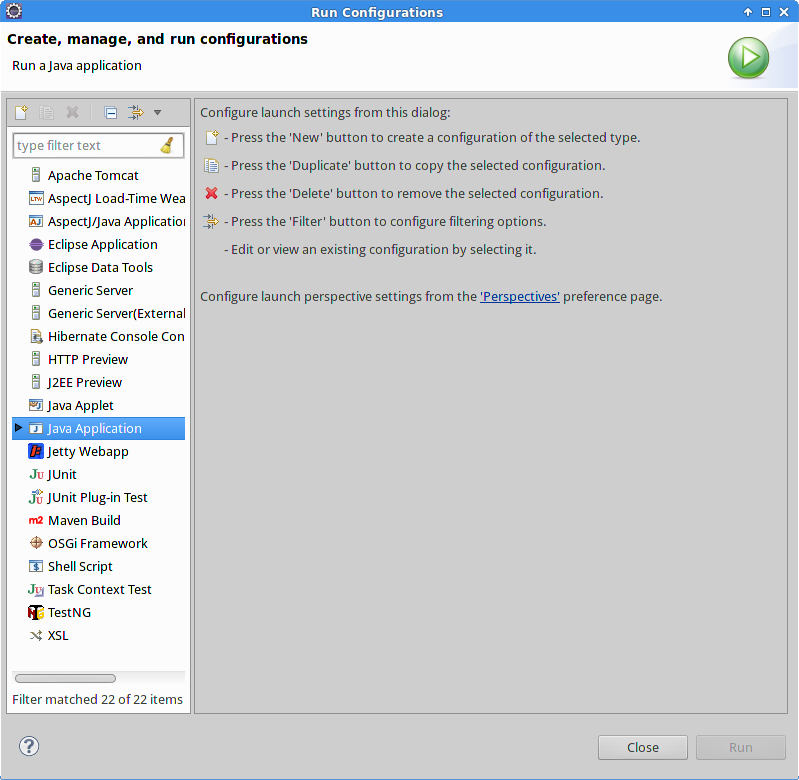
\includegraphics[width=\textwidth]{images/TheMMTkTestHarness-RunConfigurations.png}
\end{figure}

Select "Java Application" from the left-hand panel, and click the "new" icon (top left).

Fill out the Main tab as below

\begin{figure}[H]
  \centering
  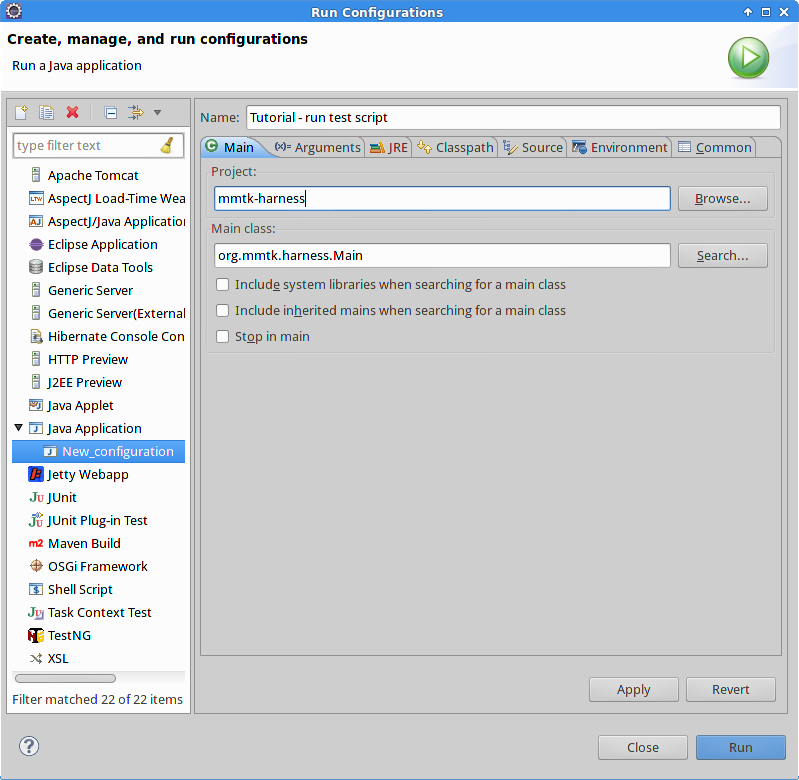
\includegraphics[width=\textwidth]{images/TheMMTkTestHarness-MainTab.png}
\end{figure}

Fill out the Arguments tab as below 

\begin{figure}[H]
  \centering
  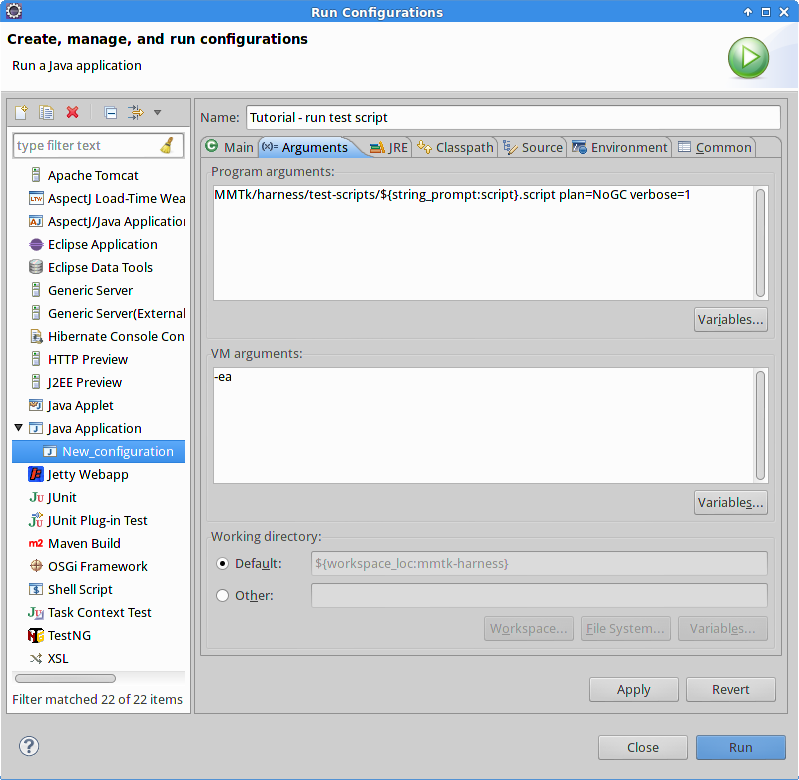
\includegraphics[width=\textwidth]{images/TheMMTkTestHarness-ArgumentsTab.png}
\end{figure}

The harness makes extensive use of the java 'assert' keyword, so you should run the harness with '-ea' in the VM options.

Click 'Apply' and then 'Run' to test the configuration.  Eclipse will prompt for a value for the 'script' variable - enter the name of one of the available test scripts, such as 'Lists', and click OK.  The scripts provided with MMTk are in the directory \spverb+MMTk/harness/test-scripts+.

You can configure eclipse to display vmmagic values (Address/ObjectReference/etc) using their toString method through the Eclipse \textrightarrow\ Preferences... \textrightarrow\ Java \textrightarrow\ Debug \textrightarrow\ Detail Formatters menu. The simplest option is to check the box to use toString 'As the label for all variables'.

\end{section}

\begin{section}{Test harness options}

Options are passed to the test harness as 'keyword=value' pairs.  The standard MMTk options that are available through JikesRVM are accepted (leave off the "-X:gc:"), as well as the following harness-specific options:

\begin{center}
\begin{longtable}{p{0.3\textwidth}p{0.6\textwidth}}
Option & Meaning \\
plan & The MMTk plan class.  Defaults to org.mmtk.plan.marksweep.MS \\
initHeap & Initial heap size.  It is also a good idea to use 'variableSizeHeap=false', since the heap growth manager uses elapsed time to make its decisions, and time is seriously dilated by the MMTk Harness. \\
maxHeap & Maximum heap size (default: 64 pages) \\
trace & Debugging messages from the MMTk Harness.  Useful trace options include
\begin{itemize}
  \item ALLOC - trace object allocation
  \item AVBYTE - Mutations of the 'available byte' in each object header
  \item COLLECT - Detailed information during GC
  \item HASH - Hash code operations
  \item MEMORY - page-level memory operations (map, unmap, zero)
  \item OBJECT - trace object mutation events 
  \item REFERENCES - Reference type processing
  \item REMSET - Remembered set processing
  \item SANITY - Gives detailed information during Harness sanity checking
  \item TRACEOBJECT - Traces every call to traceObject during GC (requires MMTk support)
\end{itemize}
    See the class org.mmtk.harness.lang.Trace for more details and trace options - most of the remaining options are only of interest to maintainers of the Harness itself. \\
watchAddress & Set a watchpoint on a given address or comma-separated list of addresses.  The harness will display every load and store to that address. \\
watchObject & Watch modifications to a given object or comma-separated list of objects, identified by object ID (sequence number). \\
gcEvery & Force frequent GCs.  Options are
\begin{itemize}
  \item ALLOC - GC after every object allocation 
  \item SAFEPOINT - GC at every GC safepoint
\end{itemize} \\
scheduler & Optionally use the deterministic scheduler.  Options are
\begin{itemize}
  \item JAVA (default) - Threads in the script are Java threads, scheduled by the host JVM
  \item DETERMINISTIC - Threads are scheduled deterministically, with yield points at every memory access.
\end{itemize} \\
schedulerPolicy & Select from several scheduling policies,
\begin{itemize}
  \item FIXED - Threads yield every 'nth' yield point
  \item RANDOM - Threads yield according to a pseudo-random policy
  \item NEVER - Threads only yield at mandatory yieldpoints
\end{itemize} \\
yieldInterval & For the FIXED scheduling policy, the yield frequency. \\
randomPolicyLength \newline randomPolicySeed \newline randomPolicyMin \newline randomPolicyMax & Parameters for the RANDOM scheduler policy.  Whenever a thread is created, the scheduler fixes a yield pattern of 'length' integers between 'min' and 'max'.  These numbers are used as yield intervals in a circular manner. \\
policyStats & Dump statistics for the deterministic scheduler's yield policy. \\
bits=32\textbar 64 & Select between 32 and 64-bit memory models. \\
dumpPcode & Dump the pseudo-code generated by the harness interpreter \\
timeout & Abort collection if a GC takes longer than this value (seconds).  Defaults to 30. \\
\end{longtable}
\end{center}

\end{section}

\begin{section}{Scripts}

The \spverb+MMTk/harness/test-scripts+ directory contains several test scripts.

\begin{table}
\centering
\begin{tabular}{p{0.22\linewidth}p{0.3\linewidth}p{0.38\linewidth}}
Script & Purpose & Description \\
Alignment & Test allocator alignment behaviour & Tests alignment by creating a list of objects aligned to a mixture of 4-byte and 8-byte boundaries. \\
CyclicGarbage & Test cycle detector in Reference Counting collectors & Creates large amounts of cyclic garbage in the form of circular linked lists. \\
FixedLive & General collection test & Harness version of the FixedLive GC micro-benchmark.  Creates a binary tree, then allocates short-lived objects to force garbage collections. \\
HashCode & Hash code test. & Creates objects and verifies that their hashcode is unchanged after a GC. \\
LargeObject & Large object allocator test & Creates objects with sizes ranging from 2 to 32 pages (8k to 128k bytes). \\
Lists & Generational collector stress test & Creates a set of lists of varying lengths, and then allocates to force collections.  Ensures that there are Mature\textrightarrow Nursery, Nursery\textrightarrow Mature and Stack\textrightarrow Nursery and Stack\textrightarrow Mature pointers at every GC.  Remsets get a serious workout. \\
OutOfMemory & Tests out-of-memory handling. & Allocates a linked list that grows until the heap fills up. \\
Quicksort & General collection test & Implements a list-based quicksort. \\
ReferenceTypes & Reference type test & Creates Weak references, forces collections and ensures that they are correctly handled. \\
Spawn & Concurrency test & Creates lots of threads which allocate objects. \\
SpreadAlloc & Free-list allocator test & Creates large numbers of objects with random size distributions, keeping a fraction of the objects alive. \\ 
SpreadAlloc16 & Concurrent free-list allocator test & A multithreaded version of SpreadAlloc. \\
\end{tabular}
\end{table}

\end{section}

\begin{section}{Scripting language}

\begin{subsection}{Basics}

The language has three types: integer, object and user-defined. The object type behaves essentially like a double array of pointers and integers (odd, I know, but the scripting language is basically concerned with filling up the heap with objects of a certain size and reachability).  User-defined types are like Java objects without methods, 'C' structs, Pascal record types etc.

Objects and user-defined types are allocated with the 'alloc' statement: alloc(p,n,align) allocates an object with 'p' pointers, 'n' integers and the given alignment; alloc(type) allocates an object of the given type.  Variables are declared 'c' style, and are optionally initialized at declaration.

User-defined types are declared as follows:

\begin{lstlisting}
type list {
  int value;
  list next;
}
\end{lstlisting}

and fields are accessed using java-style "dot" notation, eg
\begin{lstlisting}
  list l = alloc(list);
  l.value = 0;
  l.next = null;
\end{lstlisting}

At this stage, fields can only be dereferenced to one level, eg \spverb+l.next.next+ is not valid syntax - you need to introduce a temporary variable to achieve this.

Object fields are referenced using syntax like \spverb+tmp.int[5]+ or \spverb+tmp.object[i*3]+,
ie like a struct of arrays of the appropriate types.

\end{subsection}

\begin{subsection}{Syntax}

\begin{lstlisting}
script ::= (method|type)...

method ::= ident "(" { type ident { "," type ident}...  ")"
           ( "{" statement... "}"
           | "intrinsic" "class" name "method" name "signature" "(" java-class {, java class} ")"

type ::= "type" ident "{" field... "}"
field ::= type ident ";"

statement ::=
	  "if" "(" expr ")" block { "elif" "(" expr ")" block } [ "else" block ]
	| "while "(" expr ")" block
	| [ [ type ] ident "=" ] "alloc" "(" expr "," expr [ "," expr ] ")" ";"
	| [ ident "=" ] "hash" "(" expr ")" ";"
        | "gc" "(" ")"
        | "spawn" "(" ident [ "," expr ]... ")" ";"
	| type ident [ "=" expr ] ";"
	| lvalue "=" expr ";"

lvalue ::= ident "=" expr ";"
	| ident "." type "[" expr "]"

type ::= "int" | "object" | ident

expr ::= expr binop expr
		| unop expr
		| "(" expr ")"
		| ident
		| ident "." type "[" expr "]"
		| ident "." ident
		| int-const
		| intrinsic

intrinsic ::= "alloc" ( "(" expr "," expr ["," expr] ")
                      | type
                      )
            | "(" expr ")"
            | "gc " "(" ")"

binop ::= "+" | "-" | "*" | "/" | "%" | "&&" | "||" | "==" | "!="

unop ::= "!" | "-"
\end{lstlisting}

\end{subsection}

\end{section}

\begin{section}{MMTk Unit Tests}

There is a small set of unit tests available for MMTk, using the harness as scaffolding.  These tests can be run in the standard test infrastructure using the 'mmtk-unit-tests' test set, or the shell script 'bin/unit-test-mmtk'.  Possibly more usefully, they can be run from Eclipse.

To run the unit tests in Eclipse, build the mmtk harness project (see above), and add the directory \spverb+testing/tests/mmtk/src+ to your build path (navigate to the directory in the package explorer pane in eclipse, right-click \textrightarrow\ build-path \textrightarrow\ Use as Source Folder).  Either open one of the test classes, or highlight it in the package explorer and press the 'run' button.

\end{section}

\end{chapter}


\part{Architecture}
\label{part:architecture}

This section describes the architecture of Jikes RVM. The RVM can be divided into the following components:

\begin{itemize}
  \item \hyperref[cha:coreruntimeservices]{Core Runtime Services:} (thread scheduler, class loader, library support, verifier, etc.) This element is responsible for managing all the underlying data structures required to execute applications and interfacing with libraries.
  \item \hyperref[cha:magic]{Magic:} The mechanisms used by Jikes RVM to support low-level systems programming in Java.
  \item \hyperref[cha:compilers]{Compilers:} (baseline, optimizing, JNI) This component is responsible for generating executable code from bytecodes.
  \item \hyperref[cha:mmtk]{Memory managers:} This component is responsible for the allocation and collection of objects during the execution of an application.
  \item \hyperref[cha:adaptiveoptimizationsystem]{Adaptive Optimization System:} This component is responsible for profiling an executing application and judiciously using the optimizing compiler to improve its performance.
\end{itemize}

\setNextFileName{AdaptiveOptimizationSystem.html}
\begin{chapter}{Adaptive Optimization System}
\label{cha:adaptiveoptimizationsystem}

A comprehensive discussion of the design and implementation of the original Jikes RVM adaptive optimization system is given in the OOPSLA 2000 paper by Arnold, Fink, Grove, Hind and Sweeney. A number of aspects of the system have been changed since 2000, so a better resource is a technical report \href{http://domino.research.ibm.com/library/cyberdig.nsf/1e4115aea78b6e7c85256b360066f0d4/30c2b5bb5352443885256f550066b5c1%21OpenDocument}{Nov. 2004 technical report} that describes the architecture and implementation in some detail. This section of the userguide is based on section 5 of the 2004 technical report.

The implementation of the Jikes RVM adaptive optimization system uses a number of Java threads: several organizer threads in the runtime measurements component, the controller thread, and the compilation thread. The various threads are loosely coupled, communicating with each other through shared queues and/or the other in memory data structures. All queues in the system are blocking priority queues; if a consumer thread performs a dequeue operation when the queue is empty, it suspends until a producer thread performs an enqueue operation.

The adaptive optimization system performs two primary tasks: selective optimization and profile-directed inlining.

\begin{paragraph}{Selective Optimization}

The goal of selective optimization is to identify regions of code in which the application spends significant execution time (often called ``hot spots''), determine if overall application performance is likely to be improved by further optimizing one or more hot spots, and if so to invoke the optimizing compiler and install the resulting optimized code in the virtual machine.

In Jikes RVM, the unit of optimization is a method.  Thus, to perform selective optimization, first the runtime measurements component must identify candidate methods (``hot methods'') for the controller to consider. To this end, it installs a listener that periodically samples the currently executing method at every taken yieldpoint.  When it is time to take a sample, the listener inspects the thread's call stack and records a single compiled method id into a buffer. If the yieldpoint occurs in the prologue of a method, then the listener additionally records the compiled method id of the current activation's caller.  If the taken yieldpoint occurs on a loop backedge or method epilogue, then the listener records the compiled method id of the current method. 

When the buffer of samples is full, the sampling window ends. The listener then unregisters itself (stops taking samples) and wakes the sleeping Hot Method Organizer.  The Hot Method Organizer processes the buffer of compiled method ids by updating the Method Sample Data.  This data structure maintains, for every compiled method, the total number of times that it has been sampled. Careful design of this data structure (\spverb+MethodCountData.java+) was critical to achieving low profiling overhead. In addition to supporting lookups and updates by compiled method id, it must also efficiently enumerate all methods that have been sampled more times than a (varying) threshold value. After updating the Method Sample Data, the Hot Method Organizer creates an event for each method that has been sampled in this window and adds it to the controller's priority queue, using the sample value as its priority. The event contains the compiled method and the \textit{total} number of times it has been sampled  since the beginning of execution.  After enqueuing the last event, the Hot Method Organizer re-registers the method listener and then sleeps until the next buffer of samples is ready to be processed.

When the priority queue delivers an event to the controller, the controller dequeues the event and applies the model-driven recompilation policy to determine what action (if any) to take for the indicated method.  If the controller decides to recompile the method, it creates a recompilation event that describes the method to be compiled and the optimization plan to use and places it on the recompilation queue. The recompilation queue prioritizes events based on the cost-benefit computation.

When an event is available on the recompilation queue, the recompilation thread removes it and performs the compilation activity specified by the event. It invokes the optimizing compiler at the specified optimization level and installs the resulting compiled method into the VM. 

Although the overall structure of selective optimization in Jikes RVM is similar to that originally described in Arnold et al's OOPSLA 2000 paper, we have made several changes and improvements based on further experience with the system. The most significant change is that in the previous system, the method sample organizer attempted to filter the set of methods it presented to the controller.  The organizer passed along to the controller only methods considered "hot".  The organizer deemed a method "hot'' if the percentage of samples attributed to the method exceeded a dynamically adjusted threshold value. Method samples were periodically decayed to give more weight to recent samples. The controller dynamically adjusted this threshold value and the size of the sampling window in an attempt to reduce the overhead of processing the samples.

Later, significant algorithmic improvements in key data structures and additional performance tuning of the listeners, organizers, and
controller reduced AOS overhead by two orders of magnitude.  These overhead reductions obviate the need to filter events passed
to the controller.  This resulted in a more effective system with fewer parameters to tune and a sounder theoretical basis.  In general, as we gained experience with the adaptive system implementation, we strove to reduce the number of tuning  parameters.  We believe that the closer the implementation matches the basic theoretical cost-benefit model, the more likely it will perform well and make reasonable and understandable decisions.

\end{paragraph}

\begin{paragraph}{Profile-Directed Inlining}

Profile-directed inlining attempts to identify frequently traversed call graph edges, which represent caller-callee relationships, and determine whether it is beneficial to recompile the caller methods
to allow inlining of the callee methods. In Jikes RVM, profile-directed inlining augments a number of static
inlining heuristics. The role of profile-directed inlining is to identify high cost-high benefit inlining opportunities that evade the static heuristics and to predict the likely target(s) of invokevirtual and invokeinterface calls that could not be statically bound at compile time.

To accomplish this goal, the system takes a statistical sample of the method calls in the running application and maintains an approximation of the dynamic call graph based on this data. The system installs a listener that samples call edges whenever a yieldpoint is taken in the prologue or epilogue of a method. To sample the call edge, it records the compiled method id of the caller and callee methods and the offset of the call instruction in the caller's machine code into a buffer. When the buffer of samples is full, the sampling window ends.
The listener then unregisters itself (stops taking samples) and wakes an organizer to update the dynamic call graph with the new profile data. The optimizing compiler's Inline Oracle uses the dynamic call graph to guide it's inline decisions.

The system currently used is based on Arnold \& Grove's CGO 2005 paper. More details of the sampling scheme and the inlining oracle can be found there, or in the source code.

\end{paragraph}

\setNextFileName{AOSController.html}
\begin{section}{AOS Controller}
\label{sec:aoscontroller}

A primary design goal for the adaptive optimization system is to enable research in online feedback-directed optimization. Therefore, we require the controller implementation to be flexible and extensible. As we gained experience with the system, the controller component went through several major redesigns to better support our goals.

The controller is a single Java thread that runs an infinite event loop. After initializing AOS, the controller enters the event loop and attempts to dequeue an event. If no event is available, the dequeue operation blocks (suspending the controller thread) until an event is available. All controller events implement an interface with a single method: process. Thus, after successfully dequeuing an event the controller thread simply invokes its process method and then, the work for that event having been completed, returns to the top of the event loop and attempts to dequeue another event. This design makes it easy to add new kinds of events to the system (and thus, extend the controller's behavior), as all of the logic to process an event is defined by the event's process method, not in the code of the controller thread.

A further level of abstraction is accomplished by representing the recompilation strategy as an abstract class with several subclasses. The process method of a hot method event invokes methods of the recompilation strategy to determine whether or not a method should be recompiled, and if so at what optimization level. The cost-benefit model itself is also reified in a class hierarchy of models to enable extension and variation. This set of abstractions enable a single controller implementation to execute a variety of strategies.

Another useful mechanism for experimentation is the ability to easily change the input parameters to AOS that define the expected compilation rates and execution speed of compiled code for the various compilers. By varying these parameters, one can easily cause the default multi-level cost-benefit model to simulate a single-level model (by defining all but one optimization level to be unprofitable). One can also explore other aspects of the system, for example the sensitivity of the model to the accuracy of these parameters. We found this capability to be so useful that the system supports a command line argument (\spverb+-X:aos:dna=<filename>+) that causes it to optionally read these parameters from a file.

\end{section}


\NextFile{CostBenefitModel.html}
\begin{section}{Cost Benefit Model}
The Jikes RVM Adaptive Optimization System attempts to evaluate the break-even point for each action using an online competitive algorithm.  It relies on an analytic model to estimate the costs and benefits of each selective recompilation action, and evaluates the best actions according to the model predictions online.

A key advantage of this approach is that it allows a designer to extend the simple "break-even" cost-benefit model to account for more sophisticated adaptive policies, such as selective compilation with multiple optimization levels, on-stack-replacement, and long-running analyses.

In general, each potential action will incur some cost and may confer some benefit. For example, recompiling a method will certainly consume some CPU cycles, but could speed up the program execution by generating better code. In this discussion we focus on costs and benefits defined in terms of time (CPU cycles). However, in general, the controller could consider other measures of cost and benefit, such as memory footprint, garbage allocated, or locality disrupted.

The controller will take some action when it estimates the benefit to exceed the cost. More precisely, when the controller wakes at time $t$, it considers a set of $n$ available actions, the set $A = \{A_1, A_2, ..., A_n\}$. For any subset $S$ in $P(A)$, the controller can estimate the cost $C(S)$ and benefit $B(S)$ of performing all actions $A_i$ in $S$. The controller will attempt to choose the subset $S$ that maximizes $B(S) - C(S)$. Obviously $S = \{\}$ has $B(S) = C(S) = 0$; the controller takes no action if it cannot find a profitable course.

In practice, the precise cost and benefit of each action cannot be known; so, the controller must rely on estimates to make decisions.

The basic model the controller uses to decide which method to recompile, at which optimization level, and at what time is as follows.

Suppose that when the controller wakes at time $t$, and each method $m$ is currently optimized at optimization level $m_i, 0 \leq i \leq k$. Let $M$ be the set of loaded methods in the program. Let $A_{jm}$ be the action "recompile method m at optimization level $j$, or do nothing if $j = i$."

The controller must choose an action for each $m$ in $M$. The set of available actions is $Actions = \{A_{jm} | 0 \leq j \leq k, m \in M\}$.

Each action has an estimated cost and benefit: $C(A_{jm})$, the cost of taking action $A_{jm}$, for $0 \leq j \leq k$ and $T(A_{jm})$, the expected time the program will spend executing method $m$ in the future, if the controller takes action $A_{jm}$.

For $S$ in $Actions$, define $C(S) = \sum_{s \in S} C(s)$. Given $S$, for each $m$ in $M$, define $A_{min_m}$ to be the action $A_{jm}$ in $S$ that minimizes $T(A_{jm})$.  Then define $T(S) = \sum_{m \in M} T(A_{min_m})$.

Using these estimated values, the controller chooses the set $S$ that minimizes $C(S) + T(S)$. Intuitively, for each method $m$, the controller chooses the recompilation level $j$ that minimizes the expected future compilation time and running time of $m$.

It remains to define the functions $C$ and $T$ for each recompilation action. The basic model models the cost $C$ of compiling a method $m$ at level $j$ as a linear function of the size of $m$. The linear function is determined by an offline experiment to fit constants to the model.

The basic model estimates that the speedup for any optimization level $j$ is constant. The implementation determines the constant speedup factor for each optimization level offline, and uses the speedup to compute $T$ for each method and optimization level.

We assume that if the program has run for time $t$, then the program will run for another $t$ units, and then terminate. We further assume program behavior in the future will resemble program behavior in the past. Therefore, for each method we estimate that if no optimization action is performed $T(A_{jm})$ is equal to the time spent executing method $m$ so far.

Let $M=(m_1, ..., m_k)$ be the $k$ compiled methods. When the controller wakes at time $t$, each compiled method $m$ has been sampled $\sum m$ times. Let $\delta$ be the sampling interval, measured in seconds. The controller estimates that method $m$ has executed $\delta \sum m$ seconds so far, and will execute for another $\delta \sum m$ seconds in the future.

When driving recompilation based on sampling, the controller can limit its attention to the set of methods that were sampled in the previous sampling interval. This optimization does not lose precision; if the number of samples associated with a method has not changed, then the controller's estimate of the method's future execution time will not change. This implies that if the controller were to consider a
method that does not appear in the previous sampling interval, the controller would make exactly the same decision it did the last time it considered the method. This optimization, limiting the number of methods the controller must examine in each sampling interval, greatly reduces the amount of work performed by the controller.

Suppose the controller recompiles method m from optimization level $i$ to optimization level $j$ after having seen $\sum m$ samples. Let $S_i$ and $S_j $be the speedup ratios for optimization levels $i$ and $j$, respectively. After optimizing at level $j$, we adjust the sample data to represent the system state as if it had executed method $m$ at optimization level $j$ since program startup. So, we set the new number of samples for $m$ to be $\sum m \cdot (S_i/S_j)$. Thus to compute the time spent in $m$, we need know only one number, the "effective" number of samples.
\end{section}


\setNextFileName{JikesRVMsCompilers.html}
\begin{section}{Jikes RVM's compilers}
\label{sec:jikesrvmscompilers}

Jikes RVM invokes a compiler for one of three reasons. First, when the executing code reaches an unresolved reference, causing a new
class to be loaded, the class loader invokes a compiler to compile the class initializer (if one exists). Second, the system compiles each method the first time it is invoked. In these first two scenarios, the initiating application thread stalls until compilation completes.

In the third scenario, the adaptive optimization system can invoke a compiler when profiling data suggests that \textit{recompiling} a method with additional optimizations may be beneficial. The system supports both background and foreground recompilation. With background recompilation (the default), a dedicated thread asynchronously performs all recompilations.  With foreground configuration, the system invalidates a compiled method, thus, forcing recompilation at the desired optimization level at the next invocation (stalling the invoking thread until compilation completes).

The system includes two compilers with different tradeoffs between compilation overhead and code quality.
\begin{itemize}
    \item The goal of the \textit{baseline} compiler is to generate correct code quickly. For example, the IA32 baseline compiler translates bytecodes directly into native code by simulating Java's operand stack. It does not build an intermediate representation and does not perform register allocation, resulting in native code that executes only somewhat faster than bytecode interpretation.  However, it does achieve its goal of producing this code quickly, which significantly reduces the initial overhead associated with dynamic compilation.
    \item The \textit{optimizing} compiler translates bytecodes into an intermediate representation, upon which it performs a variety of optimizations.  All optimization levels include linear scan register allocation and BURS-based instruction selection. The compiler's optimizations are grouped into several levels:
      \begin{itemize}
        \item \textbf{Level 0} consists of a set of flow-sensitive optimizations performed on-the-fly during the translation from bytecodes to the intermediate representation and some additional optimizations that are either highly effective or have negligible compilation costs. The compiler performs the following optimizations during IR generation: constant, type, non-null, and copy propagation, constant folding and arithmetic simplification, branch optimizations, field analysis, unreachable code elimination, inlining of trivial methods (A trivial method is one whose body is estimated to take less code space than 2 times the size of a calling sequence and that can be inlined without an explicit guard.), elimination of redundant nullchecks, checkcasts, and array store checks.  As these optimizations reduce the size of the generated IR, performing them tends to reduce overall compilation time. Level 0 includes a number of cheap local (The scope of a local optimization is one extended basic block.) optimizations such as local redundancy elimination (common subexpression elimination, loads, and exception checks), copy propagation, constant propagation and folding. Level 0 also includes simple control flow optimizations such as static basic block splitting, peephole branch optimization, and tail recursion elimination. Finally, Level 0 performs simple code reordering, scalar replacement of aggregates and short arrays, and one pass of intraprocedural flow-insensitive copy propagation, constant propagation, and dead assignment elimination.
        \item \textbf{Level 1} resembles Level 0, but significantly increases the aggressiveness of inlining heuristics. The compiler performs both unguarded inlining of final and static methods and (speculative) guarded inlining of non-final virtual and interface methods. Speculative inlining is driven both by class hierarchy analysis and online profile data gathered by the adaptive system. In addition, the compiler exploits ``preexistence'' to safely perform unguarded inlining of some invocations of non-final virtual methods \textit{without} requiring stack frame rewriting on invalidation.  It also runs multiple passes of some of the Level 0 optimizations and uses a more sophisticated code reordering algorithm due to Pettis and Hansen.
        \item \textbf{Level 2} augments level 1 with loop optimizations such as normalization and unrolling; scalar SSA-based flow-sensitive optimizations based on dataflow, global value numbering, global common subexpression elimination, redundant and conditional branch elimination; and heap array SSA-based optimizations, such as load/store elimination, and global code placement.  \textbf{NOTE: many of the O2 optimizations are disabled by default by defining them as O3 optimizations because they are believed to be somewhat buggy.} 
      \end{itemize}
\end{itemize}

The adaptive system uses information about average compilation rate and relative speed of compiled code produced by each compiler/optimization level to make its decisions. These characteristics of the compilers are the key inputs to enable selective optimization to be effective. It allows one to employ a quick executing compiler for infrequently executed methods and an optimizing compiler for the most critical methods. See \texttt{org.jikes\-rvm.a\-dap\-ti\-ve.re\-com\-pi\-la\-tion.Com\-pi\-ler\-DNA} for the current values of these input parameters to the adaptive systems cost/benefit model.

\end{section}


// TODO convert to latex with proper inclusion of eps image which we didn't have before
Life Cycle of a Compiled Method
===============================
:author: David Grove
:date: 07-07-2008

In early implementations of Jikes RVM's adaptive system, compilation required holding a global lock that serialized compilation and also prevented classloading from occurring concurrently with compilation.  This bottleneck was removed in version 2.1.0 by switching to a finer-grained locking discipline to coordinate compilation, speculative optimization, and class loading. Since no published description of this locking protocol exists outside of the source code, we briefly summarize the life cycle of a compiled method here.

When Jikes RVM compiles a method, it creates a compiled method object to represent this particular compilation of the source method.  A compiled method has a unique id, and stores the compiled code and associated compiler meta-data. After a brief initialization phase, the compiled method transitions from uncompiled to compiling when compilation begins. During compilation, the optimizing compiler may perform speculative optimizations that can be invalidated by future class loading.  Each time the compiler so speculates, it records a relevant entry in an invalidation database.  Upon finishing compilation, the system checks to ensure that the current compilation has not already been  invalidated by concurrent classloading.  If it has not, then the system installs the compiled code, and subsequent  invocations will branch to the newly created code.

Each time a class is loaded, the system checks the invalidation database to identify the set of compiled methods to mark as obsolete,
because this classloading action invalidates speculative optimizations previously applied to that method.  A method may transition from either compiling or installed to obsolete due to a classloading-induced invalidation.  A method can also transition from installed to obsolete when the adaptive system selects a method for optimizing recompilation and a new compiled method is installed to replace it.

image:images/93224965.eps[life cycle of a compiled method]

Once a method is marked obsolete, it will never be invoked again.  However, before the generated code for the compiled method can be garbage collected, all existing invocations of the compiled method must be complete.  A compiled method transitions from obsolete to  dead when no invocations of it exist on any thread stack.  Jikes RVM detects this as part of the stack scanning phase of garbage collection; as stack frames are scanned, their compiled methods are marked as active.  Any obsolete method that is not marked as active when stack scanning completes is marked as dead and the reference to it is removed from the compiled method table.  It will then be freed during the next garbage collection


\setNextFileName{LoggingAndDebugging.html}
\begin{section}{Logging and Debugging}
\label{sec:logginganddebugging}

Complex non-deterministic systems such as the Jikes RVM adaptive system present challenges for system understanding and debugging. Virtually all of the profiling data collected by the runtime measurements component results from non-deterministic timer-based sampling at taken yieldpoints. The exact timing of these interrupts, and thus, the profile data that drives recompilation decisions, differs somewhat each time an application executes. Furthermore, many of the optimizations in the optimizing compiler rely on online profiles of conditional branch probabilities, i.e., the probabilities at the point in an execution when the recompilation occurs. Thus, because recompilations can occur at different times during each execution, a method compiled at the same optimization level could be compiled slightly differently on different runs.

The primary mechanism we use to manage this complexity is a record-replay facility for the adaptive system, where online profile data is gathered during one run and used in a subsequent run. More specifically, as methods are dynamically compiled, the system can record this information into a log file. At the end of the run, the system can optionally dump the branch probabilities of all instrumented conditional branches, the profile-derived call graph, and the profile-directed inlining decisions. This log of methods and the files of profile data can then be provided as inputs to a driver program (\texttt{org.jikes\-rvm.tools.opt.Opt\-Test\-Har\-ness}) that can replay the series of compilation actions, and then optionally execute the program. Usually a fairly rapid binary search of methods being compiled and/or the supporting profile data suffices to narrow the cause of a crash to a small set of actions taken by the optimizing compiler. Although this does not enable a perfectly accurate replay of a previous run, in practice, we have found that it suffices to reproduce almost all crashes caused by bugs in the optimizing compiler.

In addition to this record-replay mechanism, which mainly helps debugging the optimizing compiler, the adaptive system can generate a log file that contains detailed information about the actions of its organizer and controller threads. A sample is shown below:

\begin{lstlisting}
30:..7047728888 Compiled read with baseline compiler in 0.20 ms
90:..7136817287 Controller notified that read(14402) has 4.0 samples
92:..7139813016  Doing nothing cost (leaving at baseline) to read is 40.0
92:..7139830219  Compiling read cost at O0=40.42, future time=49.81
92:..7139842466  Compiling read cost at O1=65.99, future time=72.58
92:..7139854029  Compiling read cost at O2=207.44, future time=213.49
110:..7166901172 Controller notified that read(14402) has 9.0 samples
111:..7168378722  Doing nothing cost (leaving at baseline) to read=90.0
111:..7168396493  Compiling read cost at O0=40.42, future time=61.54
111:..7168409562  Compiling read cost at O1=65.99, future time=80.81
111:..7168421097  Compiling read cost at O2=207.44, future time=221.06
111:..7168435937 Scheduling level 0 recompilation of read (priority=28.46)
112:..7169879779 Recompiling (at level 0) read
114:..7173293360  Recompiled (at level 0) read
150:..7227058078 Controller notified that read(14612) has 5.11 samples
151:..7228691160  Doing nothing cost (leaving at O0) to read=51.12
151:..7228705466  Compiling read cost at O1=66.26, future time=102.14
151:..7228717124  Compiling read cost at O2=208.29, future time=241.24

<....many similar entries....>

998:..8599006259 Controller notified that read(14612) has 19.11 samples
999:..8599561634  Doing nothing cost (leaving at O0) to read=191.13
999:..8599576368  Compiling read cost at O1=54.38, future time=188.52
999:..8599587767  Compiling read cost at O2=170.97, future time=294.14
999:..8599603986 Scheduling level 1 recompilation of read (priority=2.61)
1000:..8601308856 Recompiling (at level 1) read
1002:..8604580406  Recompiled (at level 1) read
1018:..8628022176 Controller notified that read(15312) has 18.41 samples
1019:..8629548221  Doing nothing cost (leaving at O1) to read=184.14
1019:..8629563130  Compiling read cost at O2=170.97, future time=340.06
\end{lstlisting}

This sample shows an abbreviated subset of the log entries associated with the method read of the class \texttt{spec.bench\-marks.\_213\_javac.Scan\-ner\-In\-put\-Stream}, one of the hotter methods of the SPECjvm98 benchmark \spverb+_213_javac+. The first pair of numbers are the controller clock (number of timer interrupts since execution began) and the value of the hardware cycle counter (\spverb+Time.cycles()+) for the log entry. These log entries show the cost-benefit values computed by the controller for various possible optimization actions and the progression of the method from baseline compilation through two recompilations (level 0 and then at level 1). For example, at time $92$, we see four entries that give the estimated total future time (the sum of the compilation cost and the total future execution time in a method) for performing no recompilation and for each optimization level. Because the total future time for not recompiling ($40$) is less than the other alternatives ($49.81$, $72.58$, and $213.49$), the method is not scheduled for recompilation. However, at time $110$, the method has been sampled more often. Thus, the total future time estimate is updated, resulting in two recompilation actions (level 0 and level 1) that are more attractive than taking no recompilation action. Because level 0 gives the least future time, this decision is chosen by placing a recompilation event in the recompilation priority queue. The priority for the event is the expected improvement of performing this recompilation, i.e., the difference between the future time for the new level and the future time for current execution ($90 - 61.54 = 28.46$).

At clock time $150$ a similar pattern occurs when considering whether to recompile this method at level 1 or 2; initially recompiling at higher levels is not chosen (clock time $151$) until sufficient samples of the method have occurred (clock time $999$).

The figure also illustrates how samples of a method at lower optimization level are incorporated into the total samples for a method that has been recompiled. The samples at the lower level are scaled by the relative speed of the two levels as defined by the \spverb+CompilerDNA+, and used as the initial number of samples for the higher level. For example, at clock time $100$, the baseline compiled version of the method has 9 samples. When the method is recompiled at level 0, these methods are scaled down by $4.26$, which is the expected speedup defined by the \spverb+CompilerDNA+ for going from baseline to level 0, resulting in a value of $2.11$. At clock time $160$, the level 0 version of method has $5.11$ samples, i.e, $3$ additional samples of the method have occurred.

\end{section}


\setNextFileName{ThreadingAndYieldpoints.html}
\begin{section}{Threading and Yieldpoints}
\label{sec:threadingandyieldpoints}

Jikes RVM creates a native thread for each Java thread that is started. Each compiler generates yield points, which are program points where the running thread checks to determine if it should yield to another thread. The compilers insert yield points in method prologues, method epilogues, and on loop backedges.

The adaptive optimization system piggybacks on this yieldpoint mechanism to gather profile data. The thread scheduler provides an
extension point by which the runtime measurments component can install listeners that execute each time a yieldpoint is taken. Such listeners primarily serve to sample program execution to identify frequently-executed methods and call edges. Because these samples occur at well-known locations (prologues, epilogues, and loop backedges), the listener can easily attribute each sample to the appropriate Java source method.

The Jikes RVM implementation introduces a weakness with this mechanism, in that samples can only occur in regions of code that have yieldpoints.  Some low-level Jikes RVM subsystems, such as the thread scheduler and the garbage collector, elide yieldpoints because
those regions of code rely on delicate state invariants that preclude thread switching. These uninterruptible regions can distort sampling accuracy by artificially inflating the probability of sampling  the first yieldpoint executed after the program leaves an uninterruptible region of code.

\end{section}


\end{chapter}


\setNextFileName{Compilers.html}
\begin{chapter}{Compilers}
\label{cha:compilers}

\begin{itemize}
  \item \hyperref[sec:baselinecompiler]{Baseline Compiler}
  \item JNI Compiler: the JNI compiler "compiles" native methods by generating code to transition from Jikes RVM internal calling/register conventions to the native platforms ABI. It is almost completely platform-dependent.
  \item \hyperref[sec:optimizingcompiler]{Optimizing Compiler}
\end{itemize}

\setNextFileName{BaselineCompiler.html}
\begin{section}{Baseline Compiler}
\label{sec:baselinecompiler}

\begin{subsection}{General Architecture}

The goal of the baseline compiler is to efficiently generate code that is "obviously correct." It also needs to be easy to port to a new platform and self contained (the entire baseline compiler must be included in all Jikes RVM boot images to support dynamically loading other compilers). 

Roughly two thirds of the baseline compiler is machine-independent. The main file is \spverb+BaselineCompiler+ and its parent \spverb+TemplateCompilerFramework+. The main platform-dependent file is \spverb+BaselineCompilerImpl+.

Baseline compilation consists of two main steps: GC map computation (discussed below) and code generation. The code generation in the baseline compilers is mostly straightforward, consisting of a single pass through the bytecodes of the method being compiled.

Differences in the hardware architectures lead to slightly different implementation strategies for the baseline compilers. For example, the IA32 baseline compiler does not try to optimize register usage, instead the bytecode operand stack is held in memory. This leads to bytecodes that push a constant onto the stack, creating a memory write in the generated machine code. The number of memory accesses in the IA32 baseline compiler corresponds directly to the number of bytecodes. In contrast to this, the PPC baseline compiler does some register allocation of local variables (and should probably do even more register allocation to properly exploit the register set).

\spverb+TemplateCompilerFramework+ contains the main code generation switch statement that invokes the appropriate \spverb+emit<bytecode>_+ method of \texttt{Ba\-se\-li\-ne\-Com\-pi\-ler\-Impl}.

\end{subsection}

\begin{subsection}{GC Maps}

The baseline compiler computes GC maps by abstractly interpreting the bytecodes to determine which expression stack slots and local variables contain references at the start of each bytecode. There are additional compilations to handle JSRs; see the source code for details. This strategy of computing a single GC map that applies to all the internal GC points for each bytecode slightly constrains code generation. The code generator must ensure that the GC map remains valid at all GC points (including implicit GC points introduced by null pointer exceptions). It also forces the baseline compiler to report reference parameters for the various invoke bytecodes as live in the GC map for the call (because the GC map also needs to cover the various internal GC points that happen before the call is actually performed). Note that this is not an issue for the optimizing compiler which computes GC maps for each machine code instruction that is a GC point.

\end{subsection}

\end{section}


\setNextFileName{OptimizingCompiler.html}
\begin{section}{Optimizing Compiler}
\label{sec:optimizingcompiler}

The documentation for the optimizing compiler is organized into the following sections.

\begin{itemize}
  \item \hyperref[sec:methodcompilation]{Method Compilation}: The fundamental unit for compilation in the RVM is a single method.
  \item \hyperref[sec:ir]{IR}: The intermediate representation used by the optimizing compiler.
  \item \hyperref[sec:burs]{BURS}: The Bottom-Up Rewrite System (BURS) is used by the optimizing compiler for instruction selection.
  \item \hyperref[sec:opttestharness]{OptTestHarness}: A test harness for compilation parameters for specific classes and methods.
\end{itemize}

\end{section}


\setNextFileName{MethodCompilation.html}
\begin{section}{Method Compilation}
\label{sec:methodcompilation}

The fundamental unit for optimization in Jikes RVM is a single method. The optimization of a method consists of a series of compiler phases performed on the method. These phases transform the IR (intermediate representation) from bytecodes through HIR (high-level intermediate representation), LIR (low-level intermediate representation), and MIR (machine intermediate representation) and finally into machine code. Various optimizing transformations are performed at each level of IR.

An object of the class \spverb+CompilationPlan+ contains all the information necessary to generate machine code for a method. An instance of this class includes, among other fields, the \spverb+RVMMethod+ to be compiled and the array of \spverb+OptimizationPlanElements+ which define the compilation steps. The execute method of an \spverb+CompilationPlan+ invokes the optimizing compiler to generate machine code for the method, executing the compiler phases as listed in the plan's \spverb+OptimizationPlanElements+.

The \spverb+OptimizationPlanner+ class defines the standard phases used in a compilation. This class contains a static field, called \spverb+masterPlan+, which contains all possible \spverb+OptimizationPlanElements+. The structure of the master plan is a tree. Any element may either be an atomic element (a leaf of the tree), or an aggregate element (an internal node of the tree). The master plan has the following general structure:
\begin{itemize}
  \item elements which convert bytecodes to HIR
  \item elements which perform optimization transformations on the HIR
    \begin{itemize}
      \item elements which perform optimization transformations using SSA form
    \end{itemize}
  \item elements which convert HIR to LIR
  \item elements which perform optimization transformations on the LIR
    \begin{itemize}
      \item elements which perform optimization transformations using SSA form
    \end{itemize}
  \item elements which convert LIR to MIR
  \item elements which perform optimization transformations on MIR
  \item elements which convert MIR to machine code
\end{itemize}

A client (compiler driver) constructs a specific optimization plan by including all the \spverb+OptimizationPlanElements+ contained in the master plan which are appropriate for this compilation instance. Whether or not an element should be part of a compilation plan is determined by its \spverb+shouldPerform+ method. For each atomic element, the values in the \spverb+OptOptions+ object are generally used to determine whether the element should be included in the compilation plan. Each aggregate element must be included when any of its component elements must be included.

Each element must have a perform method defined which takes the IR as a parameter. It is expected, but not required, that the \spverb+perform+ method will modify the IR. The \spverb+perform+ method of an aggregate element will invoke the \spverb+perform+ methods of its elements.

Each atomic element is an object of the final class \texttt{OptimizationPlanAtomicElement}. The main work of this class is performed by its phase, an object of type \spverb+CompilerPhase+. The \spverb+CompilerPhase+ class is not final; each phase overrides this class, in particular it overrides the \spverb+perform+ method, which is invoked by its enclosing element's \spverb+perform+ method. All the state associated with the element is contained in the \spverb+CompilerPhase+; no state is in the element.

Every optimization plan consists of a selection of elements from the master plan; thus two optimization plans associated with different methods will share the same component element objects. Clearly, it is undesirable to share state associated with a particular compilation phase between two different method compilations. In order to prevent this, the perform method of an atomic element creates a new instance of its phase immediately before calling the phase's perform method. In the case where the phase contains no state the \spverb+newExecution+ method of \spverb+CompilerPhase+ can be overridden to return the phase itself rather than a clone of the phase.

\end{section}


\setNextFileName{IR.html}
\begin{section}{IR}
\label{sec:ir}

The optimizing compiler intermediate representation (IR) is held in an object of type \spverb#IR# and includes a list of instructions. Every instruction is classified into one of the pre-defined instruction formats. Each instruction includes an operator and zero or more operands. Instructions are grouped into basic blocks; basic blocks are constrained to having control-flow instructions at their end. Basic blocks fall-through to other basic blocks or contain branch instructions that have a destination basic block label. The graph of basic blocks is held in the \spverb#cfg# (control-flow graph) field of IR.

This section documents basic information about the intermediate represenation. For a tutorial based introduction to the material it is highly recommended that you read the presentation \href{http://www.jikesrvm.org/Resources/Presentations/}{Jikes RVM Optimizing Compiler Intermediate Code Representation}.

\begin{subsection}{IR Operators}

The IR operators are defined by the class \spverb#Operators#, which in turn is automatically generated from a template by a driver. The input to the driver are two files, both called \spverb#OperatorList.dat#. One input file resides in
\spverb#$RVM_ROOT/rvm/src-generated/opt-ir# and defines machine-independent operators. The other resides in
\spverb#$RVM_ROOT/rvm/src-generated/opt-ir/$\{arch\}# and defines machine-dependent operators, where \spverb#$\{arch\}# is the specific instruction architecture of interest.

Each operator in \spverb#OperatorList.dat# is defined by a five-line record, consisting of:

\begin{itemize}
  \item \spverb#SYMBOL#: a static symbol to identify the operator
  \item \spverb#INSTRUCTION_FORMAT#: the instruction format class that accepts this operator.
  \item \spverb#TRAITS#: a set of characteristics of the operator, composed with a bit-wise or (\textbar ) operator. See Operator.java for a list of valid traits.
  \item \spverb#IMPLDEFS#: set of registers implicitly defined by this operator; usually applies only to machine-dependent operators
  \item \spverb#IMPLUSES#: set of registers implicitly used by this operator; usually applies only to machine-dependent operators
\end{itemize}

For example, the entry in \spverb#OperatorList.dat# that defines the integer addition operator is
\begin{lstlisting}
INT_ADD
Binary
none
<blank line>
<blank line>
\end{lstlisting}

The operator for a conditional branch based on values of two references is defined by
\begin{lstlisting}
REF_IFCOMP
IntIfCmp
branch | conditional
<blank line>
<blank line>
\end{lstlisting}
Additionally, the machine-specific \spverb+OperatorList.dat+ file contains another line of information for use by the assembler. See the file for details.

\end{subsection}


\begin{subsection}{Instruction Format}

Every IR instruction fits one of the pre-defined \textit{Instruction Formats}. The Java package \spverb#org.jikesrvm.compilers.opt.ir# defines roughly 75 architecture\hyp independent instruction formats. For each instruction format, the package includes a class that defines a set of static methods by which optimizing compiler code can access an instruction of that format.

For example, \spverb#INT_MOVE# instructions conform to the \spverb#Move# instruction format. The following code fragment shows code that uses the \spverb#Operators# interface and the \spverb#Move# instruction format:

\begin{lstlisting}[language=Java]
import org.jikesrvm.compilers.opt.ir.*;
class X {
  void foo(Instruction s) {
    if (Move.conforms(s)) {     // if this instruction fits the Move format
      RegisterOperand r1 = Move.getResult(s);
      Operand r2 = Move.getVal(s);
      System.out.println("Found a move instruction: " + r1 + " := " + r2);
    } else {
      System.out.println(s + " is not a MOVE");
    }
  }
}
\end{lstlisting}

This example shows just a subset of the access functions defined for the Move format. Other static access functions can set each operand (in this case, \spverb#Result# and \spverb#Val#), query each operand for nullness, clear operands, create Move instructions, mutate other instructions into Move instructions, and check the index of a particular operand field in the instruction. See the Javadoc\textsuperscript{TM} reference for a complete description of the API.

Each fixed-length instruction format is defined in the text file \spverb#$RVM_ROOT/rvm/src-generated/opt-ir/InstructionFormatList.dat#. Each record in this file has four lines:

\begin{itemize}
\item \spverb#NAME#: the name of the instruction format
\item \spverb#SIZES#: the number of operands defined, defined and used, and used
\item \spverb#SIZES#: the number of operands defined, defined and used, and used
      \begin{itemize}
        \item \spverb#D/DU/U#: Is this operand a def, use, or both?
        \item \spverb#NAME#: the unique name to identify the operand
        \item \spverb#TYPE#: the type of the operand (a subclass of Operand)
        \item \spverb#[opt]#: is this operand optional?
      \end{itemize}
\item \spverb#VARSIG#: a description of repeating operands, used for variable-length instructions.
\end{itemize}

So for example, the record that defines the Move instruction format is

\begin{lstlisting}
Move
1 0 1
"D Result RegisterOperand" "U Val Operand"
<blank line>
\end{lstlisting}

This specifies that the \spverb+Move+ format has two operands, one def and one use. The def is called \spverb+Result+ and must be of type \spverb+RegisterOperand+. The use is called \spverb+Val+ and must be of type \spverb+Operand+.

A few instruction formats have variable number of operands. The format for these records is given at the top of \spverb+InstructionFormatList.dat+. For example, the record for the variable-length \spverb+Call+ instruction format is:

\begin{lstlisting}
Call
1 0 3 1 U 4
"D Result RegisterOperand" \
"U Address Operand" "U Method MethodOperand" "U Guard Operand opt"
"Param Operand"
\end{lstlisting}

This record defines the \spverb+Call+ instruction format. The second line indicates that this format always has at least 4 operands (1 def and 3 uses), plus a variable number of uses of one other type. The trailing 4 on line 2 tells the template generator to generate special constructors for cases of having 1, 2, 3, or 4 of the extra operands. Finally, the record names the \spverb+Call+ instruction operands and constrains the types. The final line specifies the name and types of the variable-numbered operands. In this case, a \spverb+Call+ instruction has a variable number of (use) operands called \spverb+Param+. Client code can access the \spverb+ith+ parameter operand of a Call instruction \spverb+s+ by calling \spverb+Call.getParam(s,i)+.

A number of instruction formats share operands of the same semantic meaning and name. For convenience in accessing like instruction formats, the template generator supports four common operand access types:
\begin{itemize}
  \item \spverb+ResultCarrier+: provides access to an operand of type \spverb+RegisterOperand+ named \spverb+Result+.
  \item \spverb+GuardResultCarrier+: provides access to an operand of type \spverb+RegisterOperand+ named \spverb+GuardResult+.
  \item \spverb+LocationCarrier+: provides access to an operand of type \spverb+LocationOperand+ named \spverb+Location+.
  \item \spverb+GuardCarrier+: provides access to an operand of type \spverb+Operand+ named \spverb+Guard+.
\end{itemize}

For example, for any instruction \spverb+s+ that carries a \spverb+Result+ operand (eg. \spverb+Move+, \spverb+Binary+, and \spverb+Unary+ formats), client code can call \spverb+ResultCarrier.conforms(s)+ and \spverb+ResultCarrier.getResult(s)+ to access the \spverb+Result+ operand.

Finally, a note on rationale. Religious object-oriented philosophers will cringe at the \spverb+InstructionFormats+. Instead, all this functionality could be implemented more cleanly with a hierarchy of instruction types exploiting (multiple) inheritance. We rejected the class hierarchy approach due to efficiency concerns of frequent virtual/interface method dispatch and type checks. Recent improvements in our interface invocation sequence and dynamic type checking algorithms may alleviate some of this concern.

\end{subsection}

\end{section}

\setNextFileName{BURS.html}
\begin{section}{BURS}
\label{sec:burs}

The optimizing compiler uses the Bottom-Up Rewrite System (BURS) for instruction selection. BURS is essentially a tree pattern matching system derived from \href{https://github.com/drh/iburg}{Iburg} by David R. Hanson. (See "Engineering a Simple, Efficient Code-Generator Generator" by Fraser, Hanson, and Proebsting, LOPLAS 1(3), Sept. 1992, doi: \href{http://dx.doi.org/10.1145/151640.151642}{10.1145/151640.151642}). The instruction selection rules for each architecture are specified in an architecture-specific file located in \texttt{\$RVM\_ROOT/rvm/src-generated/opt-burs/\$\{arch\}}, where \spverb+${arch}+ is the specific instruction architecture of interest. The rules are used in generating a parser, which transforms the IR.

Each rule is defined by a four-line record, consisting of:
\begin{itemize}
  \item \spverb+PRODUCTION+: the tree pattern to be matched. The format of each pattern is explained below.
  \item \spverb+COST+: the cost of matching the pattern as opposed to skipping it. It is a Java\textsuperscript{TM} expression that evaluates to an integer.
  \item \spverb+FLAGS+: The flags for the operation:
    \begin{itemize}
      \item \spverb+NOFLAGS+: this production performs no operation
      \item \spverb+EMIT_INSTRUCTION+: this production will emit instructions
      \item \spverb+LEFT_CHILD_FIRST+: visit child on left-and side of production first
      \item \spverb+RIGHT_CHILD_FIRST+: visit child on right-hand side of production first
    \end{itemize}
  \item \spverb+TEMPLATE+: Java code to emit
\end{itemize}

Each production has a \textit{non-terminal}, which denotes a value, followed by a colon (":"), followed by a dependence tree that produces that value. For example, the rule resulting in memory add on the Intel IA32 architecture is expressed in the following way:

\begin{lstlisting}
stm:    INT_STORE(INT_ADD_ACC(INT_LOAD(r,riv),riv),OTHER_OPERAND(r, riv))
ADDRESS_EQUAL(P(p), PLL(p), 17)
EMIT_INSTRUCTION
EMIT(MIR_BinaryAcc.mutate(P(p), IA32_ADD, MO_S(P(p), DW), BinaryAcc.getValue(PL(p))));
\end{lstlisting}

The production in this rule represents the following tree:
\begin{lstlisting}
         r     riv
          \    /
         INT_LOAD  riv
             \     /
           INT_ADD_ACC  r  riv
                    \   |  /
                   INT_STORE
\end{lstlisting}

where \spverb+r+ is a non-terminal that represents a register or a tree producing a register, riv is a non-terminal that represents a register (or a tree producing one) or an immediate value, and \spverb+INT_LOAD+, \spverb+INT_ADD_ACC+ and \spverb+INT_STORE+ are operators (terminals). \spverb+OTHER_OPERAND+ is just an abstraction to make the tree binary.

There are multiple helper functions that can be used in Java code (both cost expressions and generation templates). In all code sequences the name \spverb+p+ is reserved for the current tree node. Some of the helper methods are shortcuts for accessing properties of tree nodes:
\begin{itemize}
  \item \spverb+P(p)+ is used to access the instruction associated with the current (root) node,
  \item \spverb+PL(p)+ is used to access the instruction associated with the left child of the current (root) node (provided it exists),
  \item \spverb+PR(p)+ is used to access the instruction associated with the right child of the current (root) node (provided it exists),
    similarly,  \spverb+PLL(p)+,  \spverb+PLR(p)+,  \spverb+PRL(p)+ and  \spverb+PRR(p)+ are used to access the instruction associated with the left child of the left child, right child of the left child, left child of the right child and right child of the right child, respectively, of the current (root) node (provided they exist).
  \item \spverb+VL(p)+ is used to access the integer constant value associated with the left child of the current (root) node
  \item \spverb+VR(p)+ is used to access the integer constant value associated with the right child of the current (root) node
  \item See \spverb+BURS_Common_Helpers+ class for definitions of the helper methods
\end{itemize}

How the above rule basically reads is as follows:
If a tree shown above is seen, evaluate the cost expression (which, in this case, calls a helper function to test whether the addresses in the \spverb+STORE (P(p))+ and the \spverb+LOAD (PLL(p))+ instructions are equal. The function returns $17$ if they are, and a special value \spverb+INFINITE+ if not), and if the cost is acceptable, emit the \spverb+STORE+ instruction \spverb+(P(p))+ mutated in place into a machine-dependent add-accumulate instruction (\spverb+IA32_ADD+) that adds a given value to the contents of a given memory location.

The rules file is used to generate a file called ir.brg, which, in turn, is used to produce a file called \spverb+BURS_STATE+.java. Note that if the BURS rules are changed, it is necessary to run \spverb+ant real-clean+ in order to recreate the auto-generated Java source code for the BURS rules.

For more information on helper functions look at \spverb+BURS_Helpers.java+. For more information on the BURS algorithm see \spverb+BURS.java+.

\begin{subsection}{Future directions}

Whilst jburg allows us to do good instruction selection there are a number of areas where it is lacking:

\begin{subsubsection}{Vector operations}

We can't write productions for vector operations unless we match an entire tree of operations. For example, it would be nice to write a rule of the form:

\begin{lstlisting}
(r, r): ADD(r,r), ADD(r,r)
\end{lstlisting}

if say the architecture supported a vector add operation (ie SIMD). Unfortunately we can't have tuples on the LHS of expressions and the comma represents that matching two coverings is necessary. \href{http://doi.acm.org/10.1145/343647.343679}{Leupers} has shown how to achieve this result with a modified BURS system. Their syntax is:

\begin{lstlisting}
r: ADD(r,r)
r: ADD(r,r)
\end{lstlisting}

\end{subsubsection}

\end{subsection}

\end{section}


\setNextFileName{OptTestHarness.html}
\begin{section}{OptTestHarness}
\label{sec:opttestharness}

For optimizing compiler development, it is sometimes useful to exercise careful control over which classes are compiled, and with which optimization level. In many cases, a prototype-opt image will suit this process using the command line option \texttt{-X:aos:initial\_compiler=opt} combined with \texttt{-X:aos:enable\_recompilation=false}. This configuration invokes the optimizing compiler on each method run.The \spverb#OptTestHarness# provides even more control over the optimizing compiler. This driver program allows you to invoke the optimizing compiler as an "application" running on top of the VM.

\begin{table}
\begin{tabular}{p{0.47\linewidth}p{0.47\linewidth}}
-useBootOptions & Use the same OptOptions as the bootimage compiler. \\
-longcommandline \textless filename\textgreater & Read commands (one per line) from a file \\
+baseline & Switch default compiler to baseline \\
-baseline & Switch default compiler to optimizing \\
-load \textless class\textgreater & Load a class \\
-class \textless class\textgreater & Load a class and compile all its methods \\
-method \textless class\textgreater \textless method\textgreater  [- or \textless descrip\textgreater] & Compile method with default compiler \\
-methodOpt \textless class\textgreater \textless method\textgreater  [- or \textless descrip\textgreater] & Compile method with opt compiler \\
-methodBase \textless class\textgreater \textless method\textgreater  [- or \textless descrip\textgreater] & Compile method with base compiler \\
-er \textless class\textgreater \textless method\textgreater  [- or \textless descrip\textgreater] \{args\} & Compile with default compiler and execute a method \\
-performance & Show performance results \\
-oc & pass an option to the optimizing compiler \\
\end{tabular}
\caption{OptTestHarness command line options}
\end{table}

\begin{subsection}{Examples}

To use the OptTestHarness program:

\begin{lstlisting}
rvm org.jikesrvm.tools.oth.OptTestHarness -class Foo
\end{lstlisting}

will invoke the optimizing compiler on all methods of class \spverb#Foo#.

\begin{lstlisting}
rvm org.jikesrvm.tools.oth.OptTestHarness -method Foo bar -
\end{lstlisting}

will invoke the optimizing compiler on the first method bar of class \spverb#Foo# it loads.

\begin{lstlisting}
rvm org.jikesrvm.tools.oth.OptTestHarness -method Foo bar '(I)V;'
\end{lstlisting}

will invoke the optimizing compiler on method \spverb#Foo.bar(I)V;#.
You can specify any number of -method and -class options on the command line. Any arguments passed to OptTestHarness via -oc will be passed on directly to the optimizing compiler. So:

\begin{lstlisting}
rvm org.jikesrvm.tools.oth.OptTestHarness -oc:O1 -oc:print_final_hir=true -method Foo bar -
\end{lstlisting}

will compile \spverb#Foo.bar# at optimization level O1 and print the final HIR.

\end{subsection}

\end{section}


\end{chapter}


\setNextFileName{CoreRuntimeServices.html}
\begin{section}{Core Runtime Services}
\label{sec:coreruntimeservices}

The Jikes RVM runtime environment implements a variety of services which a Java application relies upon for correct execution. The services include:

\begin{itemize}
  \item \hyperref[sec:objectmodel]{Object Model}: The way objects are represented in storage.
  \item \hyperref[sec:classandcodemanagement]{Class and Code Management}: The mechanism for loading, and representing classes from class files. The mechanism that triggers compilation and linking of methods and subsequent storage of generated code.
  \item \hyperref[sec:threadmanagement]{Thread Management}: thread creation, scheduling and synchronization/exclusion
  \item \hyperref[sec:jni]{JNI}: Native interface for writing native methods and invoking the virtual machine from native code.
  \item \hyperref[sec:exceptionmanagement]{Exception Management}: hardware exception trapping and software exception delivery.
  \item \hyperref[sec:bootstrap]{Bootstrap}: getting an initial Java application running in a fully functional Java execution environment
  % TODO VM conventions:
\end{itemize}

The requirement for many of these runtime services is clearly visible in language primitives such as \spverb+new()+, \spverb+throw()+ and in \spverb+java.lang+ and \spverb+java.io+ APIs such as \spverb+Thread.run()+, \spverb+System.println()+, \spverb+File.open()+ etc. Unlike conventional Java APIs which merely modify the state of Java objects created by the Java application, implementation of these primitives requires interaction with and modification of the platform (hardware and system software) on which the Java application is being executed.

In addition to the services described above, Jikes RVM also provides some services that are specific to its purpose as 
a research tool:
\begin{itemize}
  \item \hyperref[sec:vmcallbacks]{VM Callbacks}: Notfications about potentially interesting events in the VM.
\end{itemize}

\end{section}


\NextFile{Magic.html}
\begin{section}{Magic}

Most Java runtimes rely upon the foreign language APIs of the underlying platform operating system to implement runtime behaviour which involves interaction with the underlying platform. Runtimes also occasionally employ small segments of machine code to provide access to platform hardware state. Note that this is expedient rather than mandatory. With a suitably smart Java bytecode compiler it would be quite possible to implement a full Java-in-Java runtime i.e. one comprising only compiled Java code (the JNode project is an attempt to implement a runtime along these lines; the Xerox, MIT, Lambda and TI Explorer Lisp machine implementations and the Xerox Smalltalk implementation were highly successful attemtps at fully compiled language runtimes).

This section provides information on \textcolor{red}{$\bigstar$} magic \textcolor{red}{$\bigstar$} which is an escape hatch that Jikes™ RVM provides to implement functionality that is not possible using the pure Java™ programming language. For example, the Jikes RVM garbage collectors and runtime system must, on occasion, access memory or perform unsafe casts. The compiler will also translate a call to Magic.threadSwitch() into a sequence of machine code that swaps out old thread registers and swaps in new ones, switching execution to the new thread's stack resumed at its saved PC

There are three mechanisms via which the Jikes RVM \textcolor{red}{$\bigstar$} magic \textcolor{red}{$\bigstar$} is implemented:
\begin{itemize}
  \item Compiler Intrinsics: Most methods are within class librarys but some functions are built in (that is, intrinsic) to the compiler. These are referred to as intrinsic functions or intrinsics.
  \item Compiler Pragmas: Some intrinsics are do not provide any behaviour but instead provide information to the compiler that modifies optimizations, calling conventions and activation frame layout. We rever to these mechanisms as compiler pragmas.
  \item Unboxed Types: Besides the primitive types, all Java values are boxed types. Conceptually, they are represented by a pointer to a heap object. However, an unboxed type is represented by the value itself. All methods on an unboxed type must be Compiler Intrinsics.
\end{itemize}

The mechanisms are used to implement the following functionality:
\begin{itemize}
  \item \hyperref[sec:rawmemoryaccess]{RawMemoryAccess}: Unfetted access to memory.
  \item Uninterruptible Code: Declaring code to be uninterruptible.
  \item Alternative Calling Conventions: Declaring different calling conventions and activation frame layout.
\end{itemize}

\end{section}

\setNextFileName{MMTk.html}
\begin{chapter}{MMTk}
\label{cha:mmtk}

% TODO missing links
The garbage collectors for Jikes RVM are provided by MMTk. The document \href{http://cs.anu.edu.au/~Robin.Garner/mmtk-guide.pdf}{MMTk: The Memory Manager Toolkit} describes MMTk and gives a tutorial on how to use and edit it and is the best place to start.  An updated version of the tutorial is available in this \hyperref[part:mmtktutorial]{guide}. A detailed description of the call chain from the compilers through to MMTk \hyperref[sec:memoryallocationinjikesrvm]{here} is another good place to start understanding how MMTk integrates with Jikes RVM.  \hyperref[sec:anatomyofagarbagecollector]{Anatomy of a Garbage Collector} describes the major building blocks of an MMTk collector and \hyperref[sec:scanningobjectsinjikesrvm]{Scanning Objects in Jikes RV}M describes how objects are scanned for their pointer fields during GC.  MMTk also has a pure Java \hyperref[cha:themmtktestharness]{test harness} that allows development of garbage collectors in an IDE like eclipse.

Jikes RVM can be configured to employ various different allocation managers taken from the MMTk memory management toolkit. Managers divide the available space up as they see fit. However, they normally subdivide the available address range to provide:
\begin{itemize}
  \item a metadata area which enables the manager to track the status of allocated and unallocated storage in the rest of the heap.
  \item an immortal data area used to service allocations of objects which are expected to persist across the whole lifetime of the Jikes RVM runtime (e.g. the boot image)
  \item a large object space used to service allocations of objects which are larger than some specified size (e.g. a virtual memory page) - the large object space may employ a different allocation and reclamation strategy to that used for other objects.
  \item a small object allocation area which may be divided into e.g.two semi spaces, a nursery space and a mature space, a set of generations, a non-relocatable buddy hierarchy etc depending upon the allocation and reclamation strategy employed by the memory manager.
  \item separate spaces for code. These are designed to exclude performance problems that can occur on some architectures when code and data are mixed. See \href{http://dl.acm.org/citation.cfm?doid=1133956.1133980}{this paper} for the original motivation and experiments for a separate code space.
\end{itemize}

Virtual memory pages are lazily mapped into the RVM's memory image as they are needed.

The main class which is used to interface to the memory manager is called \spverb+Plan+. Each flavor of the manager is implemented by substituting a different implementation of this class. Most plans inherit from class \texttt{Stop\-The\-World\-GC} which ensures that all active mutator threads (i.e. ones which do not perform the job of reclaiming storage) are suspended before reclamation is commenced. The argument passed to \spverb+-X:gc:threads+ determines the number of parallel collector threads that will be used for collection.

Generational collectors employ a plan which inherits from class \spverb+Generational+. Inter alia, this class ensures that a write barrier is employed so that updates from old to new spaces are detected.

Jikes RVM may also use the \hyperref[sec:usinggcspy]{GCSpy} visualization framework. GCSpy allows developers to observe the behavior of the heap and related data structures.


\setNextFileName{AnatomyOfAGarbageCollector.html}
\begin{section}{Anatomy of a Garbage Collector}
\label{sec:anatomyofagarbagecollector}

\textbf{** Work in progress, contributions appreciated **}
\newline

This page gives a brief outline of the major control flows in the execution of a garbage collector in MMTk.  For simplicity, we focus on the MarkSweep collector, although much of the discussion will be relevant to other collectors. 

This page assumes you have a basic knowledge of garbage collection. For those that don't, please see one of the standard texts such as \href{http://gchandbook.org/}{The Garbage Collection Handbook}.

\begin{subsection}{Structure of a Plan}

An MMTk Plan is required to provide 5 classes.  They are required to have consistent names which start with the same name and have a suffix that indicates which class it inherits from. in the case of the MarkSweep plan, the name is "MS".
\begin{itemize}
  \item \spverb+MS+ - this is a singleton class that is a subclass of \texttt{org.mmtk.plan.Plan}. This class encapsulates data structures that are shared among multiple threads.
  \item \spverb+MSMutator+ - subclass of \texttt{org.mmtk.plan.MutatorContext}.  This class encapsulates data structures that are local to a single mutator thread.  In the case of Jikes RVM, a Thread is actually a subclass of this class for efficiency reasons.
  \item \spverb+MSCollector+ - subclass of \texttt{org.mmtk.plan.CollectorContext}.  This provides thread-local data structures specific to a garbage collector thread.
  \item \spverb+MSConstraints+ - subclass of \texttt{org.mmtk.plan.PlanConstraints}.  This provides configuration information that the host virtual machine might need.  It is separated out from the Plan class in order to prevent circular class loading dependencies.
  \item \spverb+MSTraceLocal+ - subclass of \texttt{org.mmtk.plan.TraceLocal}.  This provides thread-local data structures specific to a particular way of traversing the heap. In a simple collector like MarkSweep, there is only one of these classes, but in more complex collectors there may be several. For example, in a generational collector, there will be one \texttt{TraceLocal} class for a nursery collection, and another for a full-heap collection.
\end{itemize}

The basic architecture of MMTk is that virtual address space is divided into chunks (of 4MB in a 32-bit memory model) that are managed according to a specific \textit{policy}. A policy is implemented by an instance of the \spverb+Space+ class, and it is in the policy class that the mechanics of a particular mechanism (like mark-sweep) is implemented. The task of a \spverb+Plan+ is to create the policy (\spverb+Space+) objects that manage the heap, and to integrate them into the MMTk framework.  
MMTk exposes some of this memory management policy to the host VM, by allowing the VM to specify an allocator (represented by a small integer) when allocating space.  The interface exposed to the VM allows it to choose whether an object will move during collection or not, whether the object is large enough to require special handling etc. The MMTk plan is free (within the semantic guarantees exposed to the VM) to direct each of these allocators to a particular policy.

\end{subsection}

\begin{subsection}{Policies}
A policy describes how a range of virtual address space is managed.  The base class of all policies is \texttt{org.mmtk.policy.Space}, and a particular instance of a policy is known generically as a space.  The static initializer of a \spverb+Plan+ and its subclasses define the spaces that make up an MMTk plan.  

\begin{lstlisting}[language=Java,title=MS.java]
public static final MarkSweepSpace msSpace = new MarkSweepSpace("ms", VMRequest.discontiguous());
public static final int MARK_SWEEP = msSpace.getDescriptor();
\end{lstlisting}

In this code fragment, we see the \spverb+MS+ plan defined.  Note that we generally also define a \spverb+static final+ space descriptor.  This is an optimization that allows some rapid operations on spaces.

A \spverb+Space+ is a global object, shared among multiple mutator threads.  Each policy will also have one or more thread-local classes which provide unsynchronized allocation.  These classes are subclasses of \texttt{org.mmtk.u\-ti\-li\-ty.al\-loc.Al\-loc\-a\-tor}, and in the case of MarkSweep, it is called \spverb+MarkSweepLocal+.  Instances of \spverb+MarkSweepLocal+ are created as part of a mutator context, like this

\begin{lstlisting}[language=Java,title=MSMutator.java]
protected MarkSweepLocal ms = new MarkSweepLocal(MS.msSpace);
\end{lstlisting}

The design pattern is that the local Allocator will allocate space from a thread-local buffer, and when that is exhausted it will allocate a new buffer from the global \spverb+Space+, performing appropriate locking.  The constructor of the \texttt{MarkSweepLocal} specifies the space from which the allocator will allocate global memory.

\end{subsection}

\begin{subsection}{Allocation}

MMTk provides two methods for allocating an object.  These are provided by the \texttt{MS\-Mu\-ta\-tor} class, to give each plan the opportunity to use fast, unsynchronized thread-local allocation before falling back to a slower synchronized slow-path.

The version implemented in MarkSweep looks like this:

\begin{lstlisting}[language=java,title=MSMutator.java]
public Address alloc(int bytes, int align, int offset, int allocator, int site) {
  if (allocator == MS.ALLOC_DEFAULT) {
    return ms.alloc(bytes, align, offset);
  }
  return super.alloc(bytes, align, offset, allocator, site);
}
\end{lstlisting}

The basic structure of this method is common to all MMTk plans.  First they decide whether the operation applies to this level of abstraction (\spverb+if (allocator == MS.ALLOC_DEFAULT)+), and if so, delegate to the appropriate place, otherwise pass it up the chain to the super-class.  In the case of MarkSweep, \texttt{MS\-Mu\-ta\-tor} delegates the allocation to its thread-local \texttt{MarkSweepLocal} object ms.

The alloc method of \texttt{MarkSweepLocal} is inherited from \texttt{SegregatedFreeListLocal} (mark-sweep is not the only way of managing free-list allocation), and looks like this

\begin{lstlisting}[language=Java, title=SegregatedFreeListLocal.java (simplified)]
public final Address alloc(int bytes, int align, int offset) {
  int sizeClass = getSizeClass(bytes);
  Address cell = freeList.get(sizeClass);
  if (!cell.isZero()) {
    freeList.set(sizeClass, cell.loadAddress());
    /* Clear the free list link */
    cell.store(Address.zero());
    return cell;
  }
  return allocSlow(bytes, align, offset);
}
\end{lstlisting}

This is a standard pattern for thread-local allocation: first we look in the thread-local space (line 3), and if successful return the result (lines 4-8).  If unsuccessful, we request space from the global policy via the method \spverb+Allocator.allocSlow+.  This is the common interface that all Allocators use to request space from the global policy.  This will eventually call the allocator-specific \texttt{allocSlowOnce method}.  The workings of the \texttt{allocSlowOnce} method are very policy-specific, so not appropriate to look at at this stage, but eventually all policies will attempt to acquire fresh virtual memory via the \spverb+Space.acquire+ method.

\spverb+Space.acquire+ is the only correct way for a policy to allocate new virtual memory for its own use.  


\begin{lstlisting}[language=Java,title=Space.java (simplified)]
public final Address acquire(int pages) {
  pr.reservePages(pages);
  // Poll, either fixing budget or requiring GC
  if (VM.activePlan.global().poll(false, this)) {
    VM.collection.blockForGC();
    return Address.zero(); // GC required, return failure
  }
  // Page budget is ok, try to acquire virtual memory
  Address rtn = pr.getNewPages(pagesReserved, pages, zeroed);
  if (rtn.isZero()) {  // Failed, so force a GC
    boolean gcPerformed = VM.activePlan.global().poll(true, this);
    VM.collection.blockForGC();
    return Address.zero();
  }
  return rtn;
}
\end{lstlisting}

The logic of \spverb+space.acquire+ is:
\begin{itemize}
  \item First, poll the plan to find out whether the heap is full.  This logic is performed by the plan, because it has knowledge of copy reserves etc.
  \item The \spverb+poll+ method will request a GC if required, and return \spverb+true+ if it has done so.
  \item Then we wait for GC if required. \spverb+poll+ can't wait, because it is called in circumstances that aren't GC safe.
  \item If \spverb+Plan.poll(...)+ returns \spverb+false+ (we are within the allowed heap size), we call \spverb+pr.getNewPages+ to allocate virtual memory.  At this stage we can find that we have run out of virtual memory, and if so, we force a GC
  \item If a GC is performed, we return \spverb+Address.zero()+, rather than retrying locally.  In many plans, the next allocation request will be satisfied by re-using space in a page that already belongs to a policy, so the post-GC allocation must be performed further up in the call stack. The retry logic is handled in \spverb+Allocator.allocSlowInline+.
\end{itemize}

\begin{lstlisting}[language=Java,title=Allocator.java (simplified)]
public final Address allocSlowInline(int bytes, int alignment, int offset) {
  boolean emergencyCollection = false;
  while (true) {
    Address result = allocSlowOnce(bytes, alignment, offset);
    if (!result.isZero()) {
      return result;
    }
    if (emergencyCollection) {
      VM.collection.outOfMemory();
    }
    emergencyCollection = Plan.isEmergencyCollection();
  }
}
\end{lstlisting}

This code fragment shows the retry logic in the allocator.  We try allocating using \spverb+allocSlowOnce+, which may recycle partially-used blocks and eventually call \spverb+Space.acquire+.  If a GC occurred, we try again.  Eventually the plan will request an emergency collection which will (for example) cause soft references to be dropped.  If this fails we throw an \spverb+OutOfMemoryError+.

\end{subsection}

\begin{subsection}{Collection}

\begin{subsubsection}{Scheduling}

In a stop-the-world garbage collector like MarkSweep, the mutator threads run until memory is exhausted, then all mutator threads are suspended, the collector threads are activated, and they perform a garbage collection.  After the GC is complete, the collector threads are suspended and the mutator threads resume.  MMTk also has some support for concurrent collectors, in which one or more collector threads can be scheduled to run alongside the mutator, either exclusively or in addition to (hopefully briefer) stop-the-world phases. 

Thread scheduling in MMTk is handled by a GC controller thread, implemented in the singleton class \texttt{org.mmtk.plan.ControllerCollectorContext} held in the static field \texttt{Plan.controlCollectorContext}. Whenever a collection is initiated, it is done by calling methods on this object.

\end{subsubsection}

\begin{subsubsection}{Initiating}

As mentioned above, every attempt to allocate fresh virtual memory calls the current plan's \spverb+poll(...)+ method.  This initiates a GC by calling \texttt{con\-trol\-Col\-lec\-tor\-Con\-text.re\-quest()}, which in a stop-the-world collector like MarkSweep pauses the mutator threads and then wakes the collector threads.  The main loop of the garbage collector is simply the \spverb+run()+ method of \texttt{ParallelCollector}, shown below.

\begin{lstlisting}[language=Java,title=ParallelCollector]
public void run() {
  while(true) {
    park();
    collect();
  }
}
\end{lstlisting}

The \spverb+collect()+ method is specific to the type of collector, and in \texttt{StopTheWorldCollector} it looks like this
\begin{lstlisting}[language=Java,title=StopTheWorldCollector]
public void collect() {
  Phase.beginNewPhaseStack(Phase.scheduleComplex(global().collection));
}
\end{lstlisting}

\end{subsubsection}

\begin{subsubsection}{Collector Phases}

Every garbage collection consists of a series of steps.  Each step is either executed once (e.g. updating the mark state before marking the heap), or in parallel on all available collector threads (e.g. the parallel mark phase).  The actual work of a step is done by the \texttt{collectionPhase} method of the global, collector or mutator class of a plan.

In early versions of MMTk, the main collection method was a template method, calling individual methods for each phase of the collection.  As the number of collectors in MMTk grew, this became unwieldy and has been replaced with a configurable mechanism of phases.  

The class org.mmtk.plan.Simple defines the basic structure of most of MMTk's garbage collectors.  First it defines the phases themselves,

\begin{lstlisting}[language=Java,title=Simple.java]
public static final short SET_COLLECTION_KIND = Phase.createSimple("set-collection-kind", null);
public static final short INITIATE            = Phase.createSimple("initiate", null);
public static final short PREPARE             = Phase.createSimple("prepare");
...
\end{lstlisting}

Each phase of the collection is represented by a 16-bit integer, an index into a table of \spverb+Phase+ objects.  Simple phases are scheduled, and combined into sequences, or complex phases.

\begin{lstlisting}[language=Java,title=Simple.java]
/** Ensure stacks are ready to be scanned */
protected static final short prepareStacks = Phase.createComplex("prepare-stacks", null,
    Phase.scheduleMutator    (PREPARE_STACKS),
    Phase.scheduleGlobal     (PREPARE_STACKS));
\end{lstlisting}

A simple phase can be scheduled in one of 4 ways: 
\begin{itemize}
  \item Global.  One collector thread is chosen to run the \texttt{collectionPhase} method of the global \spverb+Plan+ object.
  \item Collector.  All collector threads run \texttt{collectionPhase} of the plan's \texttt{CollectorContext} object(s).
  \item Mutator.  The collector threads run in parallel and iterate over the available \texttt{MutatorContext} objects (ie the mutator threads), and run the mutator's \texttt{collectionPhase} method.  Note that the collector threads are performing work on a per-mutator basis, because in general the mutator threads are stopped at this point.
  \item Concurrent.  The controller is requested to start a concurrent collectcor thread.
\end{itemize}

Between every phase of a collection, the collector threads rendezvous at a synchronization barrier.  The actual execution of a collector's phases is done in the method \texttt{Pha\-se.pro\-cess\-Pha\-se\-Stack}.  This method handles resuming a concurrent collection as well as running a full stop-the-world collection.

The actual work of a collection phase is done (as mentioned above) in the \texttt{collectionPhase} method of the major \texttt{Plan} classes.

\begin{lstlisting}[language=Java,title=MS.java]
@Inline
@Override
public void collectionPhase(short phaseId) {
  if (phaseId == PREPARE) {
    super.collectionPhase(phaseId);
    msTrace.prepare();
    msSpace.prepare(true);
    return;
  }
  if (phaseId == CLOSURE) {
    msTrace.prepare();
    return;
  }
  if (phaseId == RELEASE) {
    msTrace.release();
    msSpace.release();
    super.collectionPhase(phaseId);
    return;
  }
  super.collectionPhase(phaseId);
}
\end{lstlisting}

This excerpt shows how the global MS plan implements \texttt{collectionPhase}, illustrating the key phases of a simple stop-the-world collector.  The prepare phase performs tasks such as changing the mark state, the closure phase performs a transitive closure over the heap (the mark phase of a mark-sweep algorithm) and the release phase performs any post-collection steps.  Where possible, a plan is structured so that each layer of inheritance deals only with the objects it creates, i.e. the MS class operates on the \texttt{msSpace} and delegates work on all other spaces to the super-class where they are defined.  By convention the \texttt{PREPARE} phase is performed outside-in (super-class preparation first) and \texttt{RELEASE} is done inside-out (local first, super-class second).

\end{subsubsection}

\begin{subsubsection}{Tracing the heap}

The main operation of a tracing collector is the transitive closure operation where all (or a subset) of the object graph is visited.  Some collectors such as generational collectors perform these operations in more than one way, e.g. a nursery collection in a generational collector does not trace through pointers into the mature space, while a full-heap collection does.  All MMTk collectors are designed to run using several parallel threads, using data structures that have unsynchronized thread-local and synchronized global components in the same way as MMTk's policy classes.

MMTk's trace operation uses the following terminology:
\begin{itemize}
  \item An \textit{edge} is a reference in the heap from one reference field to the object (or node) it points to.
  \item \textit{Tracing} an object is the policy-defined operation performed by the collector on an object.  In a mark-sweep policy this means setting the mark state of the object.  In a copying policy this means moving the object to its new location.
  \item \textit{Scanning} is the process of identifying the reference fields of an object and processing the objects reachable from each of them.
\end{itemize}

Each distinct transitive closure operation is defined as a subclass of \textit{TraceLocal}.  The closure is performed in the \textit{collectionPhase} method of the plan-specific \textit{CollectorContext} class

\begin{lstlisting}[language=Java,title=MSCollector.java]
public void collectionPhase(short phaseId, boolean primary) {
  ...
  if (phaseId == MS.CLOSURE) {
    fullTrace.completeTrace();
    return;
  }
  ...
}
\end{lstlisting}

The initial starting point for the closure is computed by the \spverb+STACK_ROOTS+ and \spverb+ROOTS+ phases, which add root locations to a buffer by calling \texttt{Tra\-ce\-Lo\-cal.re\-port\-De\-lay\-ed\-Root\-Ed\-ge}.  The closure operation proceeds by invoking \texttt{traceObiect} on each root location (in method \texttt{processRootEdge}), and then invoking \texttt{scanObject} on each heap object encountered.  Note that the \texttt{CLOSURE} operation is performed multiple times in each GC, due to processing of reference types.

\end{subsubsection}

\end{subsection}

\end{section}


\setNextFileName{MemoryAllocationInJikesRVM.html}
\begin{section}{Memory Allocation in Jikes RVM}
\label{sec:memoryallocationinjikesrvm}

The way that objects are allocated in Jikes RVM can be difficult to grasp for someone new to the code base.  This document provides a detailed look at some of the paths through the JikesRVM - MMTk interface code to help bootstrap understanding of the process.  The process and code illustrated below is current as of March 2011, svn revision 16052 (between JikesRVM 3.1.1 and 3.1.2).

\begin{subsection}{Memory Manager Interface}

The best starting place to understand the allocation sequence is in the class \texttt{org.jikes\-rvm.mm.mm\-in\-ter\-fa\-ce.Me\-mo\-ry\-Ma\-na\-ger}, which is a facade class for the MMTk allocators.  MMTk provides a variety of memory management plans which are designed to be independent of the actual language being implemented.  The \texttt{MemoryManager} class orchestrates the services of MMTk to allocate memory, and adds the structure necessary to make the allocated memory into Java objects.

The method \texttt{allocateScalar} is where all scalar (ie non-array) objects are allocated.  The parameters of this method specify the object to be allocated in sufficient detail that when this method is compiled by the opt compiler, all of the parameters are compile-time constants, allowing maximum optimization.  Working through the body of the method,

\begin{lstlisting}[language=Java]
Selected.Mutator mutator = Selected.Mutator.get();
\end{lstlisting}

As mentioned above, MMTk provides many different memory management plans, one of which is selected at build time.  This call acquires a pointer to the thread-local per-mutator component of MMTk.  Much of MMTk's performance comes from providing unsynchronized thread-local data structures for the frequently used operations, so rather than provide a single interface object, it provides a per-thread interface object for both mutator and collector threads.

\begin{lstlisting}[language=Java]
allocator = mutator.checkAllocator(org.jikesrvm.runtime.Memory.alignUp(size, MIN_ALIGNMENT), align, allocator);
\end{lstlisting}

An MMTk plan in general provides several spaces where objects can be allocated, each with their own characteristics.  Jikes RVM is free to request allocation in any of these spaces, but sometimes there are constraints only available on a per-allocation basis that might force MMTk to override Jikes RVM's request.  For example, Jikes RVM may specify that objects allocated by a particular class are allocated in MMTk's non-moving space.  At execution time, one such object may turn out to be too large for allocation in the general non-moving space provided by that particular plan, and so MMTk needs to promote the object to the Large Object Space (LOS), which is also non-moving, but has high space overheads. This call will generally compile down to 0 or a small handful of instructions.

\begin{lstlisting}[language=Java]
Address region = allocateSpace(mutator, size, align, offset, allocator, site);
\end{lstlisting}

This calls a method of \texttt{MemoryManager}, common to all allocation methods (for Arrays and other special objects), that calls

\begin{lstlisting}[language=Java]
Address region = mutator.alloc(bytes, align, offset, allocator, site);
\end{lstlisting}

to actually allocate memory from the current MMTk plan.

\begin{lstlisting}[language=Java]
Object result = ObjectModel.initializeScalar(region, tib, size);
\end{lstlisting}

Now we call the Jikes RVM object model to initialize the allocated region as a scalar object, and then

\begin{lstlisting}[language=Java]
mutator.postAlloc(ObjectReference.fromObject(result), ObjectReference.fromObject(tib), size, allocator);
\end{lstlisting}

we call MMTk's \texttt{postAlloc} method to perform initialization that can only be performed after an object has been initialized by the virtual machine.

\end{subsection}

\begin{subsection}{Compiler integration}

The \spverb+allocateScalar+ method discussed above is only actually called from one place, the method \texttt{re\-sol\-ved\-New\-Sca\-lar(int ...)} in the class \texttt{org.jikes\-rvm.run\-ti\-me.Run\-ti\-me\-En\-try\-points}. This class provides methods that are accessed directly by the compilers, via fields in the \texttt{org.jikes\-rvm.run\-ti\-me.En\-try\-points} class. The 'resolved' part of the method name indicates that the class of object being allocated is resolved at compile time (recall that the Java Language Spec requires that classes are only loaded, resolved etc when they are needed - sometimes it's necessary to compile code that performs classloading and then allocate the object).

\spverb+RuntimeEntrypoints+ also contains an overload, \texttt{re\-sol\-ved\-New\-Sca\-lar(RVM\-Class)}, that is used by the reflection API to allocate objects. It's instructive to look at this method, as it performs essentially the same operations as the compiler when compiling the call to \texttt{re\-sol\-ved\-New\-Sca\-lar(int...)}.

Working backwards from this point requires delving into the individual compilers.

\begin{subsubsection}{Baseline Compiler}

There is a different baseline compiler for each architecture.  The relevant code in the baseline compiler for the ia32 architecture is in the class \texttt{org.jikes\-rvm.com\-pi\-lers.ba\-se\-li\-ne.ia32.Ba\-se\-li\-ne\-Com\-pi\-ler\-Impl}.  The method \texttt{e-mit\_re\-sol\-ved\_new(RVM\-Class)} is responsible for generating code to execute the \textit{new} bytecode when the target class is already resolved.  Looking at this method, you can see it does essentially what the \texttt{re\-sol\-ved\-New\-Sca\-lar(RVMClass)} method in \texttt{RuntimeEntrypoints does}, then generates machine code to perform the call to the \texttt{resolvedNewScalar} entrypoint.  Note how the work of calculating the size, alignment etc of the object is performed by the compiler, at compile time.

Similar code exists in the PPC baseline compiler.

\end{subsubsection}

\begin{subsubsection}{Optimizing Compiler}

The optimizing compiler is paradoxically somewhat simpler than the baseline compiler, in that injection of the call to the entrypoint is done in an architecture independent level of compiler IR.  (An overview of the Jikes RVM optimizing compiler can be found in the paper \href{http://suif.stanford.edu/~jwhaley/papers/javagrande99.pdf}{The Jalape\~no Dynamic Optimizing Compiler for Java}).

In HIR (the high-level Intermediate Representation), allocation is expressed as a 'new' opcode.  During the translation from HIR to LIR (Low-level IR), this and other opcodes are translated into instructions by the class \texttt{org.jikes\-rvm.com\-pi\-lers.opt.hir2lir.Ex\-pand\-Run\-time\-Ser\-vices}.  The method \texttt{per\-form(IR)} performs this translation, selecting particular operations via a large switch statement.  The \spverb+NEW_opcode+ case performs the task we're interested in, doing essentially the same job as the baseline compiler, but generating IR rather than machine instructions.  The compiler generates a 'call' operation, and then (if the compilation policy decides it's required) inlines it.

At this point in code generation, all the methods called by \texttt{Run\-ti\-me\-En\-try\-points.re\-sol\-ved\-New\-Sca\-lar(int...)} which are annotated \spverb+@Inline+ are also inlined into the current method.  This inlining extends through to the MMTk code so that the allocation sequence can be optimized down to a handful of instructions.

It can be instructive to look at the various levels of IR generated for object allocation using a simple test program and the \hyperref[subsec:opttestharness]{OptTestHarness} utility described elsewhere in the user guide.

\end{subsubsection}

\end{subsection}

\end{section}


\setNextFileName{ScanningObjectsInJikesRVM.html}
\begin{section}{Scanning Objects in Jikes RVM}
\label{sec:scanningobjectsinjikesrvm}

\end{section}


\setNextFileName{UsingGCSpyc.html}
\begin{section}{Using GCSpy}
\label{sec:usinggcspy}

% TODO fill in

\end{section}

\end{chapter}


\part{MMTk Tutorial}
\label{part:mmtktutorial}

This tutorial will build up a sophisticated garbage collector from scratch, starting with the empty shell that is the NoGC "collector" in MMTk (collector is a misnomer in this case since NoGC does not collect), and gradually adding functionality.

This tutorial will tell you the mechanics of building a collector in MMTk. It will tell you how but it does not tell you anything about why. The tutorial thus serves two purposes: 1) to give you some insight into the mechanics of MMTk (but not the underlying reasons or design rationale), and 2) show you that the mechanics of building a non-trivial GC in MMTk is not hard, hopefully giving you confidence to start exploring MMTk more deeply.

Please use the latest release to work with the tutorial. If you run into trouble following the instructions, please try again with \spverb+hg tip+. If the problem persists, please \href{http://www.jikesrvm.org/ReportingBugs/}{report this as a bug}.

\begin{enumerate}
\item \hyperref[cha:preliminaries]{Preliminaries}
\item \hyperref[cha:buildingamarksweepcollector]{Building a Mark-sweep Collector}
\item \hyperref[cha:buildingahybridcollector]{Building a Hybrid Copying/Mark-Sweep Collector}
\end{enumerate}

\setNextFileName{Preliminaries.html}
\begin{section}{Preliminaries}
\label{sec:preliminaries}

\begin{subsection}{Getting MMTk and Jikes RVM and Eclipse working}
\begin{enumerate}
  \item \hyperref[sec:getthesource]{Download} the latest Jikes RVM release (or use hg tip)
  \item Ensure you can \hyperref[sec:buildingsjikesrvm]{Build} and \hyperref[sec:runningjikesrvm]{Run the RVM}.
  \item Ensure you can build and run the BaseBaseNoGC configuration (build with: \spverb+bin/buildit localhost BaseBaseNoGC+, run with something like:
    \begin{lstlisting}
dist/BaseBaseNoGC_ia32-linux/rvm HelloWorld
    \end{lstlisting}
    Note that this configuration \textit{does not} perform garbage collection so can only run small benchmarks which do not exhaust available memory. This configuration will be used as the basis for the tutorial.
  \item Ensure that your source is \hyperref[sec:editingjikesrvminanide]{successfully imported} (and editable) within an IDE such as Eclipse.
  \item Set up an \hyperref[sec:themmtktestharness]{Eclipse Run configuration} for the \spverb+NoGC+ plan using the MMTk Test Harness.
\end{enumerate}

\end{subsection}

\begin{subsection}{Creating The Base Tutorial Collector}

\begin{enumerate}
  \item Copy the \spverb+org.mmtk.plan.nogc+ package to \spverb+org.mmtk.plan.tutorial+ (copy and paste the package in Eclipse).
  \item Rename the constituent classes from \spverb+NoGC*+ to \spverb+Tutorial*+ (use Refactor \textrightarrow\ Rename on each class within the \spverb+org.mmtk.plan.tutorial+ package in Eclipse).
  \item Edit file class \spverb+org.mmtk.harness.PlanSpecificConfig+, and add the following lines 
     \begin{lstlisting}
register(new PlanSpecific("org.mmtk.plan.tutorial.Tutorial").addExpectedSpaces("default"), "Tutorial");
     \end{lstlisting}
to the static initializer (look for "NoGC").
  \item Modify your MMTk Harness Eclipse Run Configuration to use the new Plan (the name of the plan is the second parameter to the "register" method you inserted above), and click 'Run' to run it.
  \item Build and run the resulting collector. \newline Build with something like:
    \begin{lstlisting}
bin/buildit localhost BaseBaseTutorial
    \end{lstlisting}
    run with something like:
    \begin{lstlisting}
dist/BaseBaseTutorial_ia32-linux/rvm HelloWorld
    \end{lstlisting}
\end{enumerate}

\end{subsection}

\end{section}


\setNextFileName{BuildingAMarkSweepCollector.html}
\begin{section}{Building a Mark-sweep Collector}
\label{sec:buildingamarksweepcollector}

We will now modify the \spverb+Tutorial+ collector to perform allocation and collection according to a mark-sweep policy. First we will change the allocation from bump-allocation to free-list allocation (but still no collector whatsoever), and then we will add a mark-sweep collection policy, yielding a complete mark-sweep collector.

\begin{subsection}{Free-list Allocation}

This step will change your simple collector from using a bump pointer to a free list (but still without any garbage collection).

\begin{enumerate}
  \item Update the constraints for this collector to reflect the constraints of a mark-sweep system, by updating \spverb+TutorialConstraints+ as follows:
    \begin{itemize}
      \item \spverb+gcHeaderBits()+ should return \texttt{Mark\-Sweep\-Space.LOCAL\_GC\_BITS\_REQUIRED}.
      \item \spverb+gcHeaderWords()+ should return \texttt{Mark\-Sweep\-Space.GC\_HEADER\_WORDS\_REQUIRED}.
      \item The \spverb+maxNonLOSDefaultAllocBytes()\spverb+ method should be added, overriding one provided by the base class, and should return \texttt{Se\-gre\-ga\-ted\-Free\-List\-Spa\-ce.MAX\_FREELIST\_OBJECT\_BYTES} (because this reflects the largest object size that can be allocated with the free list allocator).
    \end{itemize}
  \item In \spverb+Tutorial+, replace the \spverb+ImmortalSpace+ with a \spverb+MarkSweepSpace+:
    \begin{enumerate}
      \item rename the variable \spverb+noGCSpace+ to \spverb+msSpace+ (right-click, Refactor \textrightarrow\ Rename...)
      \item rename the variable \spverb+NOGC+ to \spverb+MARK_SWEEP+ (right-click, Refactor \textrightarrow\ Rename...)
      \item change the type and static initialization of \spverb+msSpace+ to
        \begin{lstlisting}
public static final MarkSweepSpace msSpace = new MarkSweepSpace("ms", VMRequest.discontiguous());
        \end{lstlisting}
      \item add an import for MarkSweepSpace and remove the redundant import for ImmortalSpace.
    \end{enumerate}
  \item In \spverb+TutorialMutator+, replace the \spverb+ImmortalLocal+ (a bump pointer) with a \spverb+MarkSweepLocal+ (a free-list allocator)
    \begin{enumerate}
      \item change the type of \spverb+nogc+ and change the static initializer appropriately.
      \item change the appropriate import statement from \spverb+ImmortalLocal+ to \spverb+MarkSweepLocal+.
      \item rename the variable \spverb+nogc+ to \spverb+ms+ (right-click, Refactor \textrightarrow\ Rename...)
    \end{enumerate}
  \item Also in \spverb+TutorialMutator+, fix \spverb+postAlloc()+ to initialize the mark-sweep header:
\begin{lstlisting}[language=Java] 
if (allocator == Tutorial.ALLOC_DEFAULT) {
  Tutorial.msSpace.postAlloc(ref);
} else {
  super.postAlloc(ref, typeRef, bytes, allocator);
}
\end{lstlisting}
  \item In \spverb+PlanSpecificConfig+, find the line for \spverb+Tutorial+, and change \spverb+"default"+ to \spverb+"ms"+
\end{enumerate}

With these changes, \spverb+Tutorial+ should now work, just as it did before, only exercising a free list (mark-sweep) allocator rather than a bump pointer (immortal) allocator. Create a \spverb+BaseBaseTutorial+ build, and test your system to ensure it performs just as it did before. You may notice that its memory is exhausted slightly earlier because the free list allocator is slightly less efficient in space utilization than the bump pointer allocator.

\end{subsection}

\begin{subsection}{Mark-Sweep Collection}

The next change required is to perform mark-and-sweep collection whenever the heap is exhausted. The \spverb+poll()+ method of a plan is called at appropriate intervals by other MMTk components to ask the plan whether a collection is required.
\begin{enumerate}
  \item Change \spverb+TutorialConstraints+ so that it inherits constraints from a collecting plan:
    \begin{lstlisting}[language=Java]
public class TutorialConstraints extends StopTheWorldConstraints
    \end{lstlisting}
  \item The plan needs to know how to perform a garbage collection. Collections are performed in phases, coordinated by data structures defined in \spverb+StopTheWorld+, and have global and thread-local components. First ensure the global components are behaving correctly. These are defined in \spverb+Tutorial+ (which is implicitly \textit{global}).
    \begin{enumerate}
      \item Make \spverb+Tutorial+ extend \spverb+StopTheWorld+ (for stop-the-world garbage collection) rather than \spverb+Plan+ (the superclass of \spverb+StopTheWorld+):
        \begin{lstlisting}[language=Java]
public class Tutorial extends StopTheWorld
        \end{lstlisting}
       \item Rename the trace variable to \spverb+msTrace+ (right-click, Refactor \textrightarrow\ Rename...)
       \item Add code to ensure that \spverb+Tutorial+ performs the correct global collection phases in \spverb+collectionPhase()+:
         \begin{enumerate}
           \item First remove the assertion that the code is never called (\spverb+if (VM.VERIFY_ASSERTIONS) VM.assertions._assert(false);+).
           \item Add the prepare phase, preparing both the global tracer (\spverb+msTrace+) and the space (\spverb+msSpace+), after first performing the preparation phases associated with the superclasses. Using the commented template in \spverb+Tutorial.collectionPhase()+, set the following within the clause for \spverb+phaseId == PREPARE+:
             \begin{lstlisting}[language=Java]
if (phaseId == PREPARE) {
  super.collectionPhase(phaseId);
  msTrace.prepare();
  msSpace.prepare(true);
  return;
}
             \end{lstlisting}
           \item Add the closure phase, again preparing the global tracer (\spverb+msTrace+):
             \begin{lstlisting}[language=Java]
if (phaseId == CLOSURE) {
  msTrace.prepare();
  return;
}
             \end{lstlisting}
           \item Add the release phase, releasing the global tracer (\spverb+msTrace+) and the space (\spverb+msSpace+) before performing the release phases associated with the superclass:
             \begin{lstlisting}[language=Java]
if (phaseId == RELEASE) {
  msTrace.release();
  msSpace.release();
  super.collectionPhase(phaseId);
  return;
}
             \end{lstlisting}
           \item Finally ensure that for all other cases, the phases are delegated to the superclass, uncommenting the following after all of the above conditionals:
             \begin{lstlisting}[language=Java]
super.collectionPhase(phaseId);
             \end{lstlisting}
         \end{enumerate}
       \item Add a new accounting method that determines how much space a collection needs to yield to the mutator. The method, \spverb+getPagesUsed+, overrides the one provided in the \spverb+StopTheWorld+ superclass:
         \begin{lstlisting}[language=Java]
@Override
public int getPagesUsed() {
  return super.getPagesUsed() + msSpace.getPagesUsed();
}
         \end{lstlisting}
       \item Add a new method that determines whether an object will move during collection:
         \begin{lstlisting}[language=Java]
@Override
public boolean willNeverMove(ObjectReference object) {
  if (Space.isInSpace(MARK_SWEEP, object))
    return true;
  return super.willNeverMove(object);
}
         \end{lstlisting}
    \end{enumerate}
  \item Next ensure that Tutorial correctly performs \textit{local} collection phases. These are defined in \spverb+TutorialCollector+.
    \begin{enumerate}
      \item Make \spverb+TutorialCollector+ extend \spverb+StopTheWorldCollector+:
        \begin{enumerate}
          \item Extend the class (\texttt{public class Tutorial\-Collector ex\-tends Stop\-The\-World\-Collector}).
          \item Import \spverb+StopTheWorldCollector+.
          \item Remove some methods now implemented by \texttt{Stop\-The\-World\-Col\-lec\-tor}: \spverb+collect()+ and (if present) \spverb+concurrentCollect()+ and \newline \spverb+concurrentCollectionPhase()+.
        \end{enumerate}
      \item Add code to ensure that \spverb+Tutorial+ performs the correct global collection phases in \spverb+collectionPhase()+:
        \begin{enumerate}
           \item First remove the assertion that the code is never called (\spverb+if (VM.VERIFY_ASSERTIONS) VM.assertions._assert(false);+).
           \item Add the prepare phase, preparing both the local tracer (\spverb+trace+) after first performing the preparation phases associated with the superclasses. Using the commented template in \spverb+TutorialCollector.collectionPhase()+, set the following within the clause for \spverb+phaseId == PREPARE+:
             \begin{lstlisting}[language=Java]
if (phaseId == Tutorial.PREPARE) {
  super.collectionPhase(phaseId, primary);
  trace.prepare();
  return;
}
             \end{lstlisting}
           \item Add the closure phase, completing the local tracer (\spverb+trace+):
             \begin{lstlisting}[language=Java]
if (phaseId == Tutorial.CLOSURE) {
  trace.completeTrace();
  return;
}
             \end{lstlisting}
           \item Add the release phase, releasing the local tracer (\spverb+trace+) before performing the release phases associated with the superclass:
             \begin{lstlisting}[language=Java]
if (phaseId == Tutorial.RELEASE) {
  trace.release();
  super.collectionPhase(phaseId, primary);
  return;
}
             \end{lstlisting}
           \item Finally ensure that for all other cases, the phases are delegated to the superclass, uncommenting the following after all of the above conditionals:
             \begin{lstlisting}[language=Java]
super.collectionPhase(phaseId, primary);
             \end{lstlisting}
         \end{enumerate}
    \end{enumerate} 
  \item Finally ensure that \spverb+Tutorial+ correctly performs local mutator-related collection activities:
    \begin{enumerate}
      \item Make \spverb+TutorialMutator+ extend \spverb+StopTheWorldMutator+:
        \begin{enumerate}
          \item Extend the class: \texttt{pu\-blic class Tu\-to\-rial\-Mu\-ta\-tor ex\-tends Stop\-The\-World\-Mu\-ta\-tor}.
          \item Import \spverb+StopTheWorldMutator+.
        \end{enumerate}
      \item Update the mutator-side collection phases:
        \begin{enumerate}
          \item First remove the assertion that the code is never called (\spverb+if (VM.VERIFY_ASSERTIONS) VM.assertions._assert(false);+).
          \item Add the prepare phase to \spverb+collectionPhase()+ which prepares mutator-side data structures (namely the per-thread free lists) for the startof a collection:
            \begin{lstlisting}[language=Java]
if (phaseId == Tutorial.PREPARE) {
  super.collectionPhase(phaseId, primary);
  ms.prepare();
  return;
}
            \end{lstlisting}
          \item Add the release phase to \spverb+collectionPhase()+ which re-initializes mutator-side data structures (namely the per-thread free lists) after the end of a collection:
            \begin{lstlisting}[language=Java]
if (phaseId == Tutorial.RELEASE) {
  ms.release();
  super.collectionPhase(phaseId, primary);
  return;
}
            \end{lstlisting}
          \item Finally, delegate all other phases to the superclass:
            \begin{lstlisting}[language=Java]
super.collectionPhase(phaseId, primary);
            \end{lstlisting}
        \end{enumerate}
    \end{enumerate}
\end{enumerate}

With these changes, \spverb+Tutorial+ should now work with both mark-sweep allocation \textit{and} collection. Create a \spverb+BaseBaseTutorial+ build, and test your system to ensure it performs just as it did before. You can observe the effect of garbage collection as the program runs by adding \spverb+-X:gc:verbose=1+ to your command line as the first argument after \spverb+rvm+. If you run a very simple program (such as \spverb+HelloWorld+), you might not observe any garbage collection. In that case, try running a larger program such as a DaCapo benchmark. You may also observe that the output from \spverb+-X:gc:verbose=1+ indicates that the heap is growing. Dynamic heap resizing is normal default behavior for a JVM. You can override this by providing minimum (\spverb+-Xms+) and maximum (\spverb+-Xmx+) heap sizes (these are standard arguments respected by all JVMs. The heap size should be specified in bytes as an integer and a unit (K, M, G), for example: \spverb+-Xms20M -Xmx20M+.

\end{subsection}

\begin{subsection}{Optimized Mark-sweep Collection}

MMTk has a unique capacity to allow specialization of the performance-critical scanning loop. This is particularly valuable in collectors which have more than one mode of collection (such as in a generational collector), so each of the collection paths is explicitly specialized at build time, removing conditionals from the hot portion of the tracing loop at the core of the collector. Enabling this involves just two small steps:
\begin{enumerate}
  \item Indicate the number of specialized scanning loops and give each a symbolic name, which at this stage is just one since we have a very simple collector:
    \begin{enumerate}
      \item Override the \spverb+numSpecializedScans()+ getter method in \texttt{Tu\-to\-rial\-Con\-strain\-ts}:
        \begin{lstlisting}[language=Java]
@Override
public int numSpecializedScans() { return 1; }
        \end{lstlisting}
      \item Define a constant to represent our (only) specialized scan in \spverb+Tutorial+ (we will call this scan "mark"):
        \begin{lstlisting}[language=Java]
public static final int SCAN_MARK = 0;
        \end{lstlisting}
     \end{enumerate}
  \item Register the specialized method:
    \begin{enumerate}
      \item Add the following line to \spverb+registerSpecializedMethods()+ method in \spverb+Tutorial+:
        \begin{lstlisting}[language=Java]
TransitiveClosure.registerSpecializedScan(SCAN_MARK, TutorialTraceLocal.class);
        \end{lstlisting}
      \item Add \spverb+Tutorial.SCAN_MARK+ as the first argument to the superclass constructor for \spverb+TutorialTraceLocal+:
        \begin{lstlisting}[language=Java]
public TutorialTraceLocal(Trace trace) {
  super(Tutorial.SCAN_MARK, trace);
}
        \end{lstlisting}
    \end{enumerate}
\end{enumerate}

\end{subsection}

\end{section}


\setNextFileName{BuildingAHybridCollector.html}
\begin{section}{Building a Hybrid Collector}
\label{sec:buildingahybridcollector}

Extend the Tutorial plan to create a "copy-MS" collector, which allocates into a copying nursery and at collection time, copies nursery survivors into a mark-sweep space. This plan does not require a write barrier (it is not strictly generational, as it will collect the whole heap each time the heap is full). Later we will extended it with a write barrier, allowing the nursery to be collected in isolation. Such a collector would be a generational mark-sweep collector, similar to GenMS.

\begin{subsection}{Add a Copying Nursery}

This step will change your simple collector from using a bump pointer to a free list (but still without any garbage collection).

\begin{enumerate}
  \item In \spverb+TutorialConstraints+, make the following changes:
    \begin{enumerate}
      \item Override the \spverb+movesObjects()+ method to return \spverb+true+, reflecting that we are now building a copying collector:
        \begin{lstlisting}[language=Java]
@Override
public boolean movesObjects() { return true; }
        \end{lstlisting}
      \item Remove the restriction on default alloc bytes (since default allocation will now go to a bump-pointed space). To do this, remove the override of \spverb+maxNonLOSDefaultAllocBytes()+.
      \item Add a restriction on the maximum size that may be copied into the (default) non-LOS mature space:
        \begin{lstlisting}[language=Java]
@Override
public int maxNonLOSCopyBytes() { return SegregatedFreeListSpace.MAX_FREELIST_OBJECT_BYTES;}
        \end{lstlisting}
    \end{enumerate}
  \item In \spverb+Tutorial+, add a nursery space:
    \begin{enumerate}
      \item Create a new space, \spverb+nurserySpace+, of type \spverb+CopySpace+. The new space will initially be a from-space, so provide \spverb+false+ as the third argument. Initialize the space with a contiguous virtual memory region consuming 0.15 of the heap by passing "0.15" and "true" as arguments to the constructor of VMRequest(more on this later). Create and initialize a new integer constant to hold the descriptor for this new space:
        \begin{lstlisting}[language=Java]
public static final CopySpace nurserySpace = new CopySpace("nursery", false, VMRequest.highFraction(0.15f));
public static final int NURSERY = nurserySpace.getDescriptor();
        \end{lstlisting}
      \item Add the necessary import statements
      \item Add \spverb+nurserySpace+ to the \spverb+PREPARE+ and \spverb+RELEASE+ phases of \texttt{col\-lec\-tion\-Pha\-se()}, prior to the existing calls to msTrace. Pass true to nurserySpace.prepare() indicating that the nursery is a \textit{from-space} during collection.
      \item Fix accounting so that \spverb+Tutorial+ accounts for space consumed by \spverb+nurserySpace+:
         \begin{enumerate}
           \item Add \spverb+nurserySpace+ to the equation in \spverb+getPagesUsed()+
         \end{enumerate}
      \item Since initial allocation will be into a copying space, we need to account for copy reserve:
         \begin{enumerate}
           \item Add a method to override \texttt{get\-Col\-lec\-tion\-Re\-serve()} which returns \texttt{nur\-se\-ry\-Spa\-ce.re\-ser\-ved\-Pa\-ges() + su\-per.get\-Col\-lec\-tion\-Re\-ser\-ve()}
           \item Add a method to override \spverb+getPagesAvail()+, returning \texttt{get\-To\-tal\-Pa\-ges() - get\-Pa\-ges\-Re\-ser\-ved()) >> 1};
         \end{enumerate}
    \end{enumerate}
\end{enumerate}

\end{subsection}

\begin{subsection}{Add nursery allocation}

In \spverb+TutorialMutator+, replace the free-list allocator (\spverb+MarkSweepLocal+) with a nursery allocator: Use an instance of \spverb+CopyLocal+, calling it \spverb+nursery+. The constructor argument should be \texttt{Tu\-to\-rial.nur\-se\-ry\-Spa\-ce}:
  \begin{enumerate}
    \item change \spverb+alloc()+ to use \spverb+nursery.alloc()+ rather than \spverb+ms.alloc()+.
    \item remove the call to \spverb+msSpace.postAlloc()+ from \spverb+postAlloc()+ since there is no special post-allocation work necessary for the new copy space. The call to \spverb+super.postAlloc()+ should remain conditional on \spverb+allocator != Tutorial.ALLOC_DEFAULT+.
    \item change the check within \spverb+getAllocatorFromSpace()+ to check against \texttt{Tu\-to\-rial.nur\-se\-ry\-Spa\-ce} and to return \spverb+nursery+.
    \item adjust \spverb+collectionPhase+
      \begin{enumerate}
        \item replace call to \verb+ms.prepare()+ with \verb+nursery.reset()+
        \item remove call to \verb+ms.release()+ since there are no actions necessary for the nursery allocator upon release.
      \end{enumerate}
  \end{enumerate}
\end{subsection}

\begin{subsection}{Add copying to the collector}

In \spverb+TutorialCollector+ add the capacity for the collector to allocate (copy), since our new hybrid collector will perform copying.

\begin{enumerate}
  \item Add local allocators for both large object space and the mature space:
    \begin{lstlisting}[language=Java]
private final LargeObjectLocal los = new LargeObjectLocal(Plan.loSpace);
private final MarkSweepLocal mature = new MarkSweepLocal(Tutorial.msSpace);
    \end{lstlisting}
  \item Add an \spverb+allocCopy()+ method that conditionally allocates to the LOS or mature space:
    \begin{lstlisting}[language=Java]
@Override
public final Address allocCopy(ObjectReference original, int bytes,
                               int align, int offset, int allocator) {
  if (allocator == Plan.ALLOC_LOS)
    return los.alloc(bytes, align, offset);
  else
    return mature.alloc(bytes, align, offset);
}
    \end{lstlisting}
  \item Add a \spverb+postCopy()+ method that conditionally calls LOS or mature space post-copy actions:
    \begin{lstlisting}[language=Java]
@Override
public final void postCopy(ObjectReference object, ObjectReference typeRef,
                           int bytes, int allocator) {
if (allocator == Plan.ALLOC_LOS)
  Plan.loSpace.initializeHeader(object, false);
else
  Tutorial.msSpace.postCopy(object, true);
}
    \end{lstlisting}
\end{enumerate}

\end{subsection}

\begin{subsection}{Make necessary changes to TutorialTraceLocal}

\begin{enumerate}
  \item Add nurserySpace clauses to \spverb+isLive()+ and \spverb+traceObject()+:
     \begin{enumerate}
       \item Add the following to \spverb+isLive()+:
          \begin{lstlisting}[language=Java]
if (Space.isInSpace(Tutorial.NURSERY, object))
  return Tutorial.nurserySpace.isLive(object);
          \end{lstlisting}
       \item Add the following to traceObject():
          \begin{lstlisting}[language=Java]
if (Space.isInSpace(Tutorial.NURSERY, object))
  return Tutorial.nurserySpace.traceObject(this, object, Tutorial.ALLOC_DEFAULT);
          \end{lstlisting}
      \end{enumerate}
  \item Add a new \spverb+willNotMoveInCurrentCollection()+ method, which identifies those objects which do not move (necessary for copying collectors):
    \begin{lstlisting}[language=Java]
@Override
public boolean willNotMoveInCurrentCollection(ObjectReference object) {
  return !Space.isInSpace(Tutorial.NURSERY, object);
}
    \end{lstlisting}
  \item Modify \spverb+PlanSpecificConfig+ to add the new \spverb+nursery+ space:
    \begin{lstlisting}[language=Java]
new PlanSpecific("org.mmtk.plan.tutorial.Tutorial").addExpectedSpaces("ms", "nursery"), "Tutorial");
    \end{lstlisting}
\end{enumerate}

With these changes, \spverb+Tutorial+ should now work. You should be able to again build a \spverb+BaseBaseTutorial+ image and test it against any benchmark. Again, if you use \spverb+-X:gc:verbose=3+ you can see the movement of data among the spaces at each garbage collection.

\end{subsection}

\end{section}


\end{document}
